% Options for packages loaded elsewhere
\PassOptionsToPackage{unicode}{hyperref}
\PassOptionsToPackage{hyphens}{url}
\PassOptionsToPackage{dvipsnames,svgnames,x11names}{xcolor}
\documentclass[
]{report}
\usepackage{xcolor}
\usepackage[margin=25mm]{geometry}
\usepackage{amsmath,amssymb}
\setcounter{secnumdepth}{-\maxdimen} % remove section numbering
\usepackage{iftex}
\ifPDFTeX
  \usepackage[T1]{fontenc}
  \usepackage[utf8]{inputenc}
  \usepackage{textcomp} % provide euro and other symbols
\else % if luatex or xetex
  \usepackage{unicode-math} % this also loads fontspec
  \defaultfontfeatures{Scale=MatchLowercase}
  \defaultfontfeatures[\rmfamily]{Ligatures=TeX,Scale=1}
\fi
\usepackage{lmodern}
\ifPDFTeX\else
  % xetex/luatex font selection
\fi
% Use upquote if available, for straight quotes in verbatim environments
\IfFileExists{upquote.sty}{\usepackage{upquote}}{}
\IfFileExists{microtype.sty}{% use microtype if available
  \usepackage[]{microtype}
  \UseMicrotypeSet[protrusion]{basicmath} % disable protrusion for tt fonts
}{}
\makeatletter
\@ifundefined{KOMAClassName}{% if non-KOMA class
  \IfFileExists{parskip.sty}{%
    \usepackage{parskip}
  }{% else
    \setlength{\parindent}{0pt}
    \setlength{\parskip}{6pt plus 2pt minus 1pt}}
}{% if KOMA class
  \KOMAoptions{parskip=half}}
\makeatother
\usepackage{longtable,booktabs,array}
\newcounter{none} % for unnumbered tables
\usepackage{calc} % for calculating minipage widths
% Correct order of tables after \paragraph or \subparagraph
\usepackage{etoolbox}
\makeatletter
\patchcmd\longtable{\par}{\if@noskipsec\mbox{}\fi\par}{}{}
\makeatother
% Allow footnotes in longtable head/foot
\IfFileExists{footnotehyper.sty}{\usepackage{footnotehyper}}{\usepackage{footnote}}
\makesavenoteenv{longtable}
\usepackage{graphicx}
\makeatletter
\newsavebox\pandoc@box
\newcommand*\pandocbounded[1]{% scales image to fit in text height/width
  \sbox\pandoc@box{#1}%
  \Gscale@div\@tempa{\textheight}{\dimexpr\ht\pandoc@box+\dp\pandoc@box\relax}%
  \Gscale@div\@tempb{\linewidth}{\wd\pandoc@box}%
  \ifdim\@tempb\p@<\@tempa\p@\let\@tempa\@tempb\fi% select the smaller of both
  \ifdim\@tempa\p@<\p@\scalebox{\@tempa}{\usebox\pandoc@box}%
  \else\usebox{\pandoc@box}%
  \fi%
}
% Set default figure placement to htbp
\def\fps@figure{htbp}
\makeatother
\setlength{\emergencystretch}{3em} % prevent overfull lines
\providecommand{\tightlist}{%
  \setlength{\itemsep}{0pt}\setlength{\parskip}{0pt}}
\usepackage{mathtools}
\usepackage{mathrsfs}
\let\mathscr\symscr
\providecommand{\minf}{\mathscr C_\infty}
\setmainfont{DejaVuSerifCondensed.ttf}[BoldFont=DejaVuSerifCondensed-Bold.ttf,ItalicFont=DejaVuSerifCondensed-Italic.ttf,BoldItalicFont=DejaVuSerifCondensed-BoldItalic.ttf]
\setsansfont{Segoe UI}
\setmonofont{DejaVuSansMono.ttf}[Scale=0.82,BoldFont=DejaVuSansMono-Bold.ttf,ItalicFont=DejaVuSansMono-Oblique.ttf,BoldItalicFont=DejaVuSansMono-BoldOblique.ttf]
\newfontfamily\SourceLocatorFont{DejaVuMathTeXGyre.ttf}
\AtBeginDocument{\renewcommand{\UrlFont}{\SourceLocatorFont}}
\usepackage{newunicodechar}
\newunicodechar{ℓ}{\ensuremath{\ell}}
\newunicodechar{⋊}{\ensuremath{\rtimes}}
\newunicodechar{〈}{\ensuremath{\langle}}
\newunicodechar{〉}{\ensuremath{\rangle}}
\newunicodechar{𝓕}{\ensuremath{\mathcal F}}
\newunicodechar{𝔑}{\ensuremath{\mathfrak N}}
\newunicodechar{−}{\ensuremath{-}}
\newunicodechar{→}{\ensuremath{\to}}
\newunicodechar{↦}{\ensuremath{\mapsto}}
\newunicodechar{⊕}{\ensuremath{\oplus}}
\newunicodechar{⊗}{\ensuremath{\otimes}}
\newunicodechar{∎}{\ensuremath{\blacksquare}}
\setlength{\emergencystretch}{5em}
\newcommand{\sourcehash}[1]{\ifmmode\text{\nolinkurl{#1}}\else\nolinkurl{#1}\fi}
\usepackage{bookmark}
\IfFileExists{xurl.sty}{\usepackage{xurl}}{} % add URL line breaks if available
\urlstyle{same}
\hypersetup{
  colorlinks=true,
  linkcolor={Maroon},
  filecolor={Maroon},
  citecolor={Blue},
  urlcolor={Blue},
  pdfcreator={LaTeX via pandoc}}

\author{}
\date{}

\begin{document}

{
\setcounter{tocdepth}{2}
\tableofcontents
}
\chapter{Deligne weight control and the original-zeta receiving
maps}\label{deligne-weight-control-and-the-original-zeta-receiving-maps}

The current request is to read Deligne's weight-control argument
completely, reconstruct its mechanism, and prove the available
comparisons with the user's construction. This reader contains the full
new derivations. The cumulative companion,
RECONSTRUCTION\_AND\_WEIGHT\_FULL.md, includes their earlier programme
proof sources and all preceding retained mathematics.

The entire current French transcription of Pierre Deligne's \emph{La
conjecture de Weil. II}, printed pages137--252, has been read. It is a
local transcription, not original author TeX. Its identity, exact
coverage, and formula checks are recorded in
DELIGNE\_FULL\_READING\_LOG.md and
DELIGNE\_WEIGHT\_SOURCE\_READING.json. The unchanged original source
package remains available locally. A companion task's original
published-page reading of printed pp137--252, with separately recorded
formula-image checks is separately attributed in that log; root has not
independently read those scans. That comparison corrects the earlier
attribution of two source displays to transcription alone. Deligne's
cited upstream SGA, class-field and representation-theoretic results are
identified as inputs, rather than represented as newly proved from
foundations. The paper's later applications were read; this reader
reconstructs the weight-control argument and the mixed-duality
comparisons used here, not every subsequent application of the paper.

The user's complete argument and correction chain remain separately
preserved in USER\_CONSTRUCTION\_FULL\_LOGBOOK.md, with its source
receipt. The current mathematical input respects the order in that
argument: complete timing and its global quotient precede the arithmetic
interpretation. Later arithmetic calculations state when they use the
already reconstructed complete cyclic source. They do not supply
cyclicity by assuming observed prime coordinates. The supporting datum
is always \(\tau\langle Z_1;\text{no }Z_2\rangle\). Its addition remains
retracted. None of the constructions installs an arithmetic zero,
vector, midpoint, or distance on that supporting datum.

{\def\LTcaptype{none} % do not increment counter
\begin{longtable}[]{@{}
  >{\raggedright\arraybackslash}p{(\linewidth - 2\tabcolsep) * \real{0.5000}}
  >{\raggedright\arraybackslash}p{(\linewidth - 2\tabcolsep) * \real{0.5000}}@{}}
\toprule\noalign{}
\begin{minipage}[b]{\linewidth}\raggedright
Proof
\end{minipage} & \begin{minipage}[b]{\linewidth}\raggedright
Source argument and actual comparison
\end{minipage} \\
\midrule\noalign{}
\endhead
\bottomrule\noalign{}
\endlastfoot
DP0--DP9 & Determinant characters, central monodromy, all even tensor
powers, full cohomological trace formula, exterior powers and pointwise
purity; Weil II §§1.3--1.5. \\
DMG0--DMG7 & Nonsplit geometric monodromy radical, dominant pullback,
compact normalizer, and the determinant criterion for an étale
extension; completes the needed group arguments in §1.3. \\
DLM1--DLM15 & Nilpotent logarithm, primitive decomposition, exact Tate
factors, tensor and dual identities, local purity and the mixed relative
filtration; §§1.6--1.9. \\
DB0--DB10 and DBC1--DBC11 & Full positive prime-power measures,
compact-group characters, boundary nonvanishing, the exceptional
quadratic character and strict cohomological weight inequality;
§§2.1--2.2. \\
DW0--DW11 & Every singular-fibre contribution, the product and pencil,
complete Leray and Künneth terms, repeated tensor improvement, duality
and the fundamental direct-image theorem; §§3.1--3.3. \\
MDB0--MDB11 & Actual maps from the CC stalk through its recovered
arithmetic to étale fibres; mixed filtration, strictness, six-functor
duality, arithmetic costalks and full Tate/cohomological shifts; §§3.4
and6.1--6.2. \\
DC0--DC12 & The full local invariant-cycle quotient and lift:
Hochschild--Serre, localization, both Tate twists, the complete
specialization kernel, and separation of the target's weights from the
obstruction's weights; §3.6. \\
DR0--DR7 & Invertible comparison of the full integer count and
prime-power measures with Deligne's §2.1.9 measure, the original
\(-\zeta'/\zeta\), retained unit and completion factors, and exact
branchwise compatibility. \\
\end{longtable}
}

The cumulative reader additionally includes ZLB0--ZLB11, ZTM0--ZTM11,
GLB0--GLB8 and GSL0--GSL11. These give complete proofs of the
original-germ boundary, the character-shifted finite and algebraic
lifts, the whole Fréchet source boundary, and the continuous equivariant
splitting of the original and translated zero divisors. GSL constructs
an entire separator with controlled strip growth, its full quotient
inverse, and a Mellin-source representative. Its uniqueness proof uses
the actual global resolvent. It retains all multiplicities and never
replaces the source topology by an unrestricted jet product. ZLB and GLB
identify the nonzero boundary of a particular analytic eigenfunction
extension; no map identifies that extension with the user's requested
geometric lift. GSL's vanishing extension class concerns the explicitly
constructed translated-divisor sequence. Its identification with
Deligne's localization cross has not been constructed.

The later geometric comparisons construct the evaluated CC charts (CGT),
the exact degree-class comparison with the continuous lift (GTZ), and
the descended conic with its full integral fibre at2 (CD). The conic's
Tate factor comes from its actual hyperplane class; the original product
is ζ(s)ζ(s−1), with all local factors. CS and CSL construct the original
CC coefficient sheaf, its finite-unit source, four endpoint lines and
all supported-cohomology maps. Their ordinary cohomology is calculated
before any closure operation. The complete SSI theorem, independently
rederived in ESI, then proves the summation image is already closed by
constructing a continuous inverse in the actual Schwartz space. CS11 and
CSL10 carry this stronger theorem through the receiving maps.

The prime-indexed endpoint directions in CS2A remain explicit. They
arise when rational-scaling relations are generated only by moment-null
sources; allowing full Schwartz generators changes that source quotient
by exactly the displayed direct sum of endpoint pairs. This distinction
is independent of the closedness of the overlap summation image. The
source-reading record states the author's omitted generator-domain
convention and the proved comparison, rather than concealing it in
notation.

The finite-field source obtains equality of Frobenius moduli through its
cohomological argument. In the reconstructed arithmetic comparison, MDB5
proves the full costalk \(Ri_p^!E=E(-1)[-2]\) and MDB9 computes its
eigenvalue action \(\alpha\mapsto p/\alpha\), in degree two. The
conjugate-realization comparison is \(a\mapsto p/\overline a\), with the
Tate factor retained. DR proves the full original-zeta receiving map;
MDB11 gives the local Euler factors of the actual constant coefficient
object on the recovered arithmetic scheme. These proofs have not
identified the analytic zero-jet receiver with the proper arithmetic
cohomology used by Deligne's purity theorem, and do not claim an RH
resolution. The failure of one observation functor to retain weights is
calculated in MDB10; it is not a rejection of every enriched
construction on the support.

CSB calculates every retained prime endpoint action and gives the full
comparison with the earlier FR15--FR25 proof: the source LF quotient
retains those classes, whereas the specified weighted periodization
seminorm kills exactly them. CSP then constructs the inverse-image sheaf
on the evaluated complex projective line. Its degree-one cohomology is
the original quotient Q, its degree-two cohomology is the full overlap A
with the geometric covering factor, and an actual sheaf quotient
produces Q in degree two. The explicit translated-Mellin map identifies
this latter normal quotient with the earlier GSL kernel. The support,
full stalk, two cohomological degrees and their quotient maps remain
explicit; the actual antiholomorphic mirror has the opposite
sphere-orientation sign from the holomorphic swap.

CW proves the actual quotient-sheaf degree-one lift: the cohomology map
is the identity of Q, and its connecting map Q→J(−1) is zero. The
simultaneous source complexes give an explicit lift of every class.
Independently, the full original-zeta resolvent proves that every
continuous complex-linear arithmetic-equivariant map Q→J(−1) is zero,
without a density assumption about finite zero blocks. The full kernel
J(−1) retains character quotients at every complex exponent, so the
narrower weight interval of Q(−1) is not assigned to that kernel. CW
computes the exact quotient map into GSL, all its kernel and image, and
the difference between this cohomological lift and choosing
representatives equivariantly in A. Its comparison with Deligne retains
the actual obstruction quotient and both Tate factors.

CDW constructs the derived direct image itself by one resolution
compatible on both pole charts and their punctured overlap. Its strict
continuous splitting retains the winding class, both mirror actions, the
geometric degree factor and the entire source extension in both internal
degrees. The comparison between the angular class and positive sphere
integration has sign −1, which remains in the translated-zeta map. CDI
then calculates the complete continuous dual coefficient and support
complexes, including the dual cone and all endpoint factors. RD
constructs the original-zeta residue pairing with every multiplicity and
its exact nonzero block determinant; its finite-jet functionals are
dense for the weak dual topology. The residue action and normal
contragredient differ by the explicitly retained factor a². These are
constructed comparison maps; a finite-dimensional étale support-duality
realization is not asserted.

SDT subsequently proves the stronger topology from the actual weighted
coefficient space: bounded quotient sets have compact closure, and every
compact set has a compact lift constructed by a convergent sequence of
finite choices. This proves that the induced dual topology in CDI3 is
the full strong dual topology. A proof of strong reflexivity then
upgrades the finite-jet functionals to strong density. The explicitly
stated residue topology on finite-support classes has completion equal
to the entire continuous dual; it is not substituted for the inherited
topology of those classes. The reflected and unreflected residue maps
have their exact, different arithmetic covariance laws. Thus CDI and
RD's earlier restricted strong-topology claims remain accurate and are
strengthened by the complete subsequent proof.

The figures are diagrams of the proved objects and maps, not geometric
metrics on the supporting point. Their reproducible Python sources, PNG
and SVG outputs accompany this reader. DELIGNE\_COMPLETE\_BUILD.json
records every cumulative proof input and output hash. Earlier editions
remain in the local history directory.

CSD now realizes the continuous dual by an actual sheaf of functionals
on compactly supported tests. Its positive Dirac Gysin, pole stalk and
costalk maps, global comparison and inverse, and all support signs are
proved explicitly. SDT gives the full strong coefficient topologies; the
stable local cohomology topology is specified without assuming that
arbitrary germ limits preserve it. The proper current pushforward is the
transpose of pullback on tests, including both mirror orientations.

GTR then constructs the weighted trace of each recovered integer cover
on the entire coefficient sheaf, including both ramified stalks and all
their endpoint coordinates. Its inverse coefficient action gives the
factor n in the original reflected residue covariance. The complete
residue topology is written out, and the geometric action extends to its
entire strong-dual completion. The Mellin transpose and normal-dual
inclusion are explicit in this comparison. These results realize the
earlier coefficient duality and residue actions by constructed geometric
maps. The weight-control goal remains active: no nondegenerate bilinear
evaluation is promoted to a positive Hermitian form.

VSD and CV construct the ordinary dual of the actual
infinite-coefficient sheaf, and a literal morphism from its
continuous-current dual. The entire difference is computed, including
the pole Gysin maps. The original Mellin multiplication operator acts
rationally on its extra algebraic coefficient sector: every nonzero
polynomial in that operator is invertible. Its proof uses continuous
division on the complete original source and its full vanishing-jet
ideal. It follows that enlarging the dual adds no finite-dimensional
invariant sectors for this operator. Every endpoint, scalar shift and
mirror action has a stated formula; mirror action sends the rational
variable t to 1−t. The associated figure displays the actual comparison
cone and the distinct strong and weak residue completions.

GTR11 also upgrades the trace calculation to the actual derived direct
image: its trace is n times the inverse of the proved pullback, with the
intermediate direct-image identification written out. It preserves the
entire source sequence, rather than only an independently computed list
of cohomology groups.

The primal generator family GCF/PGF constructs the exact original-zeta
divisor map for all parameters and jet orders, with its original
meromorphic target and every cancellation frame. The family cokernel has
length rm at a multiplicity-m zero, while its fibre and its derived
fibre kernel each have dimension min(r,m). The full source boundary
explains the difference. It is a different boundary from CW's geometric
lift; the manuscript supplies both maps and preserves their actual
domains. The figure primal\_generator\_family.png displays these maps
without assigning coordinates or a metric to the parityless support.

CP computes the actual derived spectral obstruction of that current
inclusion. The two-term free resolution retains both the polynomial
kernel and cokernel. The computed comparison defect makes both vanish,
and the proof corrects an algebraic spectral cocycle to a continuous one
by an explicit boundary. The resulting continuous cohomology class is
unique. For each actual zero the full multiplicity, every local/global
degree, and the nonzero source cokernel are calculated; all dilation and
mirror matrices remain. This is a separation-based vanishing theorem for
the actual comparison map. CP11 gives its exact relation to Deligne's
mechanism and retains the distinction from the still unfinished
arithmetic weight-control application.

The actual polynomial localization calculation CLP derives every degree
and boundary of the constructed sphere-sheaf row, keeping its full
kernel. It proves the separated normal comparison at original zeros and
computes the distinct nonzero spectral boundary at translated zeros. The
full derived extension and the coherent-family Hom contraction identify
exactly what vanishes and what remains. Its figure
localization\_spectral\_weights.png retains the complete original-zeta
multiplier and the inverse derivative matrix. The weight separation
proved for these particular maps does not identify the whole row with
Deligne's inertia cross.

The complete-module continuation GMS combines the full global
interpolation multiplier with the actual localization complexes. GMS4
proves derived Hom vanishing with an explicit bar homotopy; GMS5 gives
the complete normal comparison inverse, retaining the whole ideal. GMS6
computes precisely the nonzero extension and the multiplier pushout that
splits. GMS8 supplies the full original-source integral, while
GMS9--GMS10 retain endpoints, cover factors and mirror actions. The
diagram global\_multiplier\_separation.png shows these maps and their
proof locators.

The complete-source continuation FOD and NEA retains the entire
intersection kernel and computes both actual extension components.
FOD2--FOD5 construct the pullbacks, pushouts and exact annihilator
ideals, distinguishing the original component preserved by the separator
from the normal component it annihilates. NEA3--NEA7 identify the exact
normal cyclic class module, all multiplicity probes and its full-source
algebraic resolvent. FOD7 and NEA10 prove the actual localization lift
from the complete original quotient. Their diagram is
full\_source\_obstruction.png. Postcomposition is distinguished from
conjugation, and the actual Deligne specialization/inertia comparison
retains its separate unfinished scope.

The local-receiver continuation LNC, LVD and RGR follows FOD/NEA with
the actual universal-cover specialization, exact local/global
comparison, continuous-dual arrows and original residue pairing. LNC4
computes the invariant-cycle cross on the actual coefficient sheaf.
LVD5--7 prove the difference between local sheaf pairings and the
nonzero global pairing, then construct their exact morphism quotient.
RGR3--10 construct the signed Gysin receiver and its relation to the
original transposed coefficient extension. RGR11 retains a separate
receiver for the already calculated positive-adjoint defect. The source
and target of each map matter: the total residue class and that defect
are different. The complete RTT, GTAH, GIQ and PCJ supporting files are
retained alongside the main proofs. The figure
local\_residue\_receiver.png identifies the exact comparison maps.
Reich's original v4 author TeX and intact source archive are included,
with read ranges in NEARBY\_CYCLES\_SOURCE\_READING\_PUBLIC.json. No
whole-paper Reich reading or arithmetic weight vanishing is claimed.

\begin{figure}
\centering
\pandocbounded{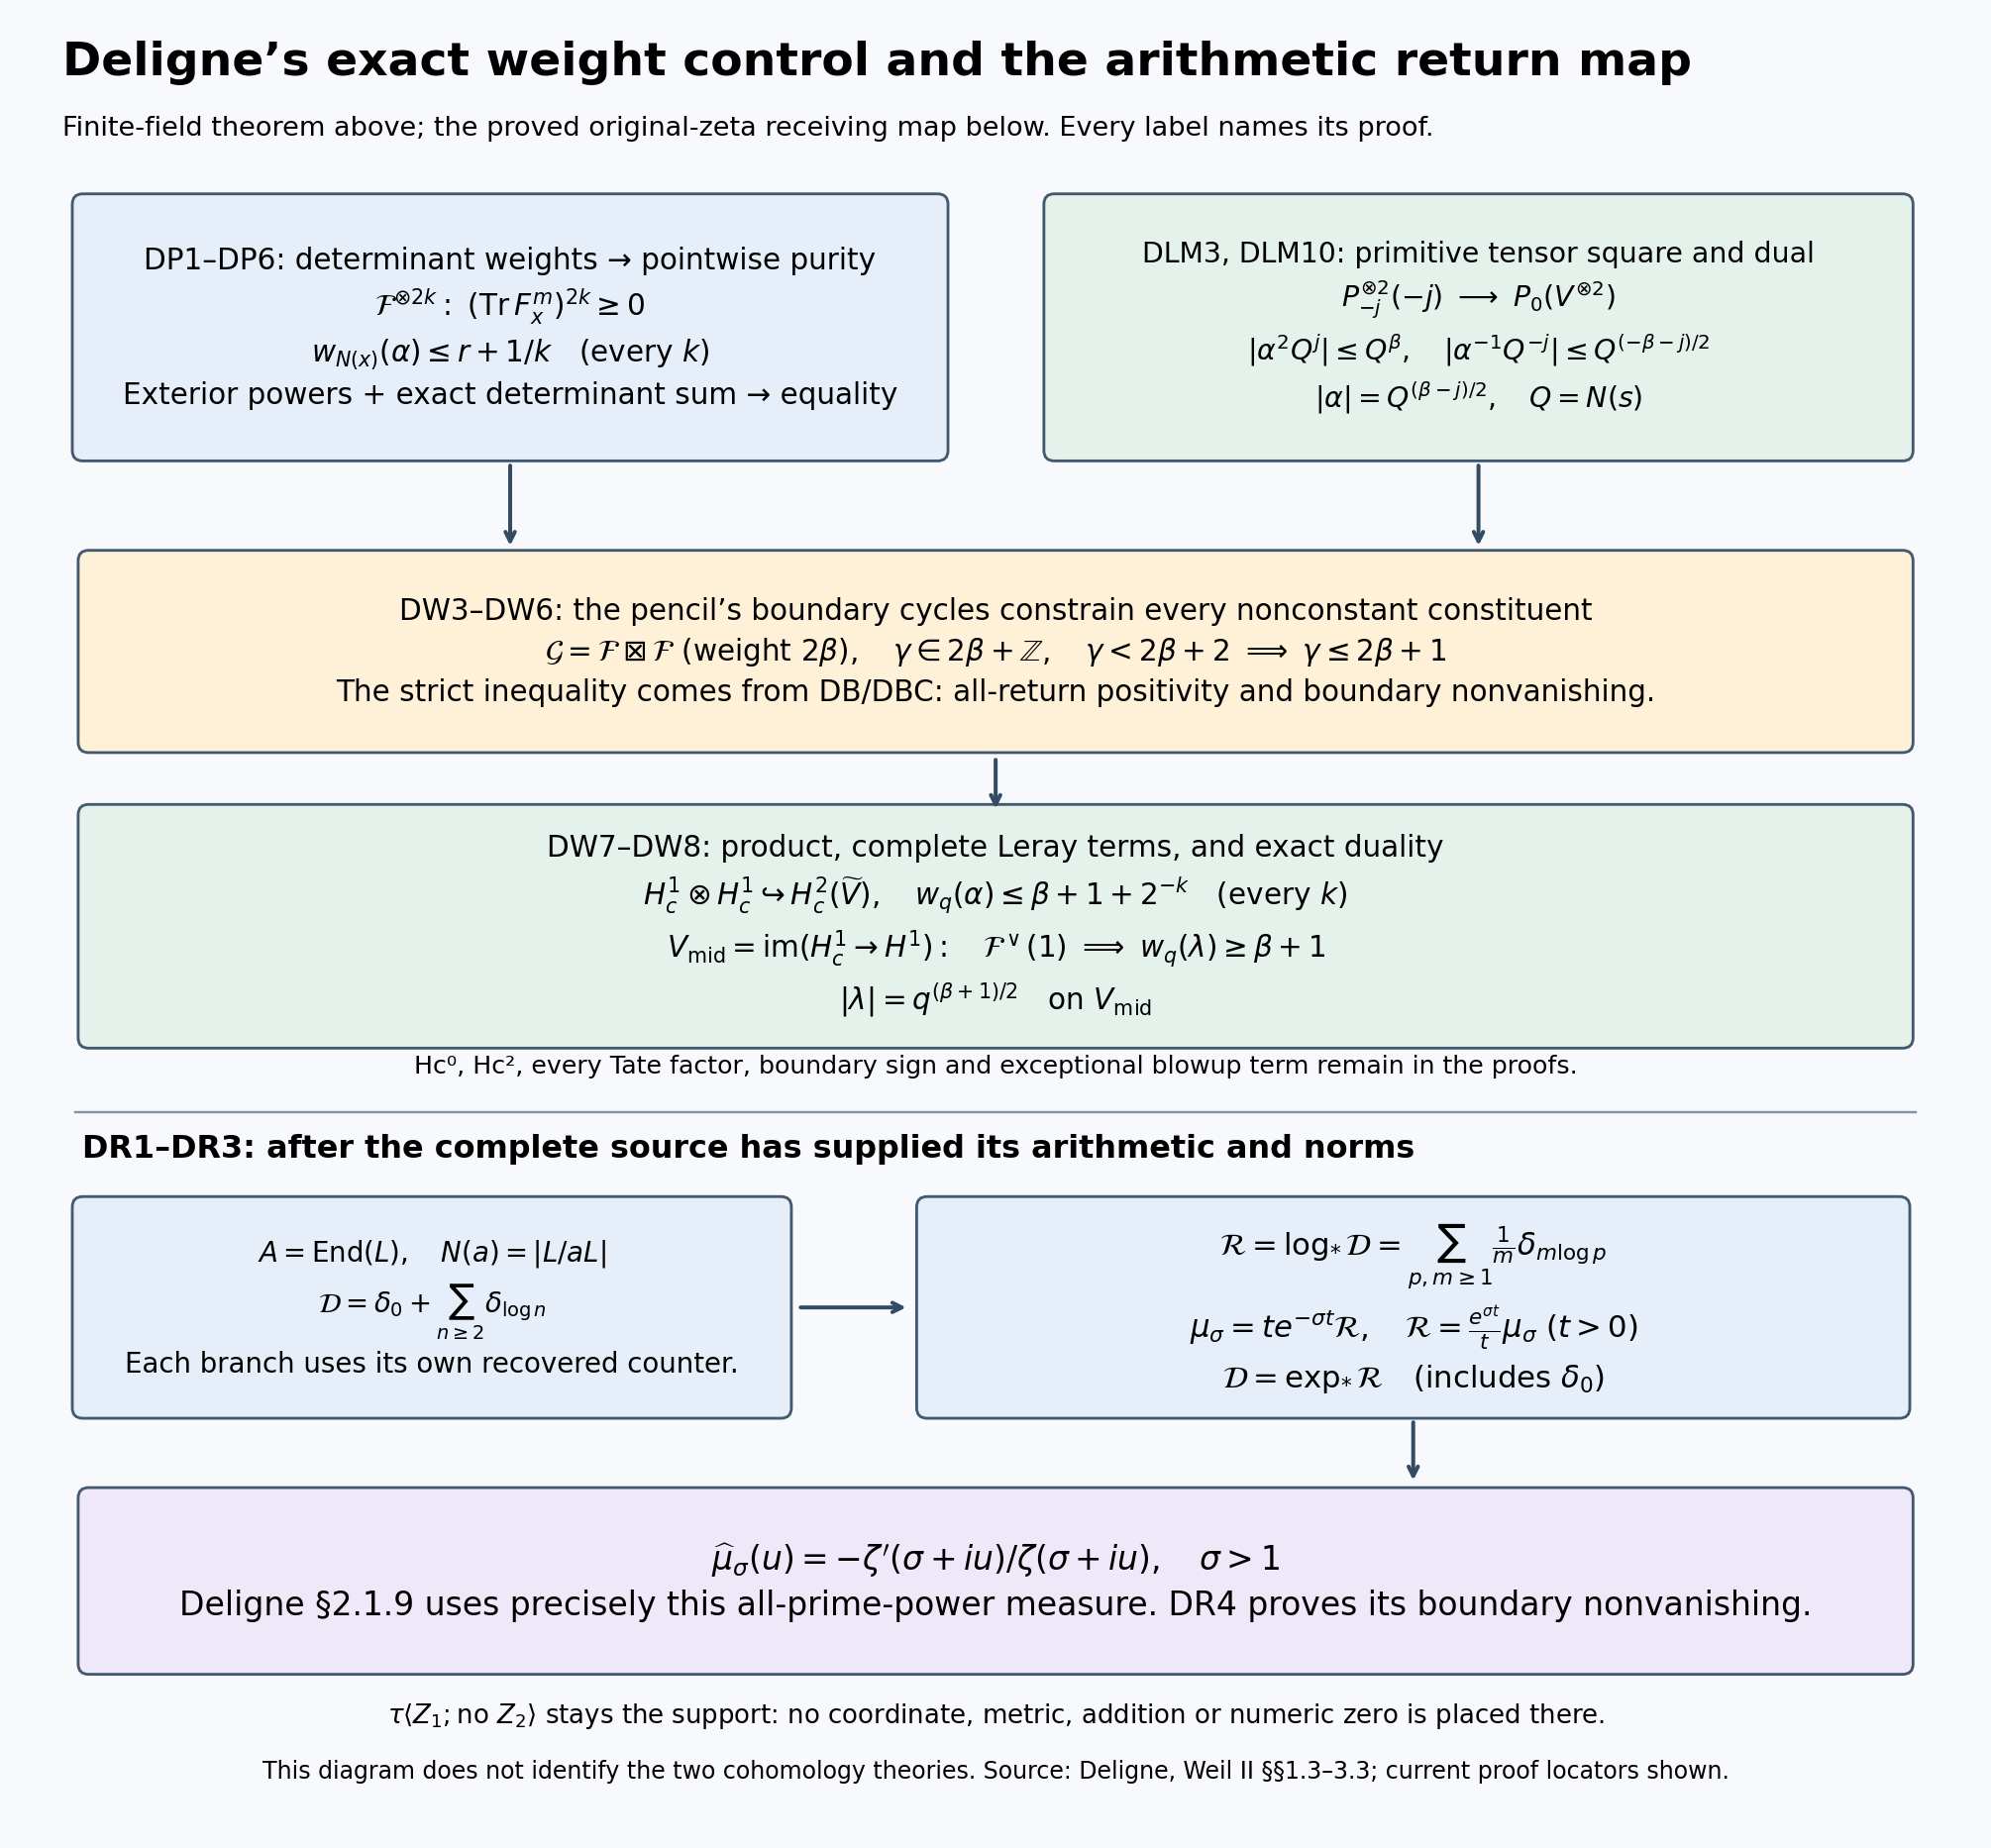
\includegraphics[keepaspectratio,alt={The exact weight mechanism and arithmetic return map}]{deligne_weight_mechanism.png}}
\caption{The exact weight mechanism and arithmetic return map}
\end{figure}

The figure records the proved maps, with their source and proof
locators. The exact purity circle in DW8 concerns the indicated middle
cohomology; it is not asserted for every compactly supported cohomology
class. The diagram assigns no metric or coordinate to the supporting
point.

\begin{figure}
\centering
\pandocbounded{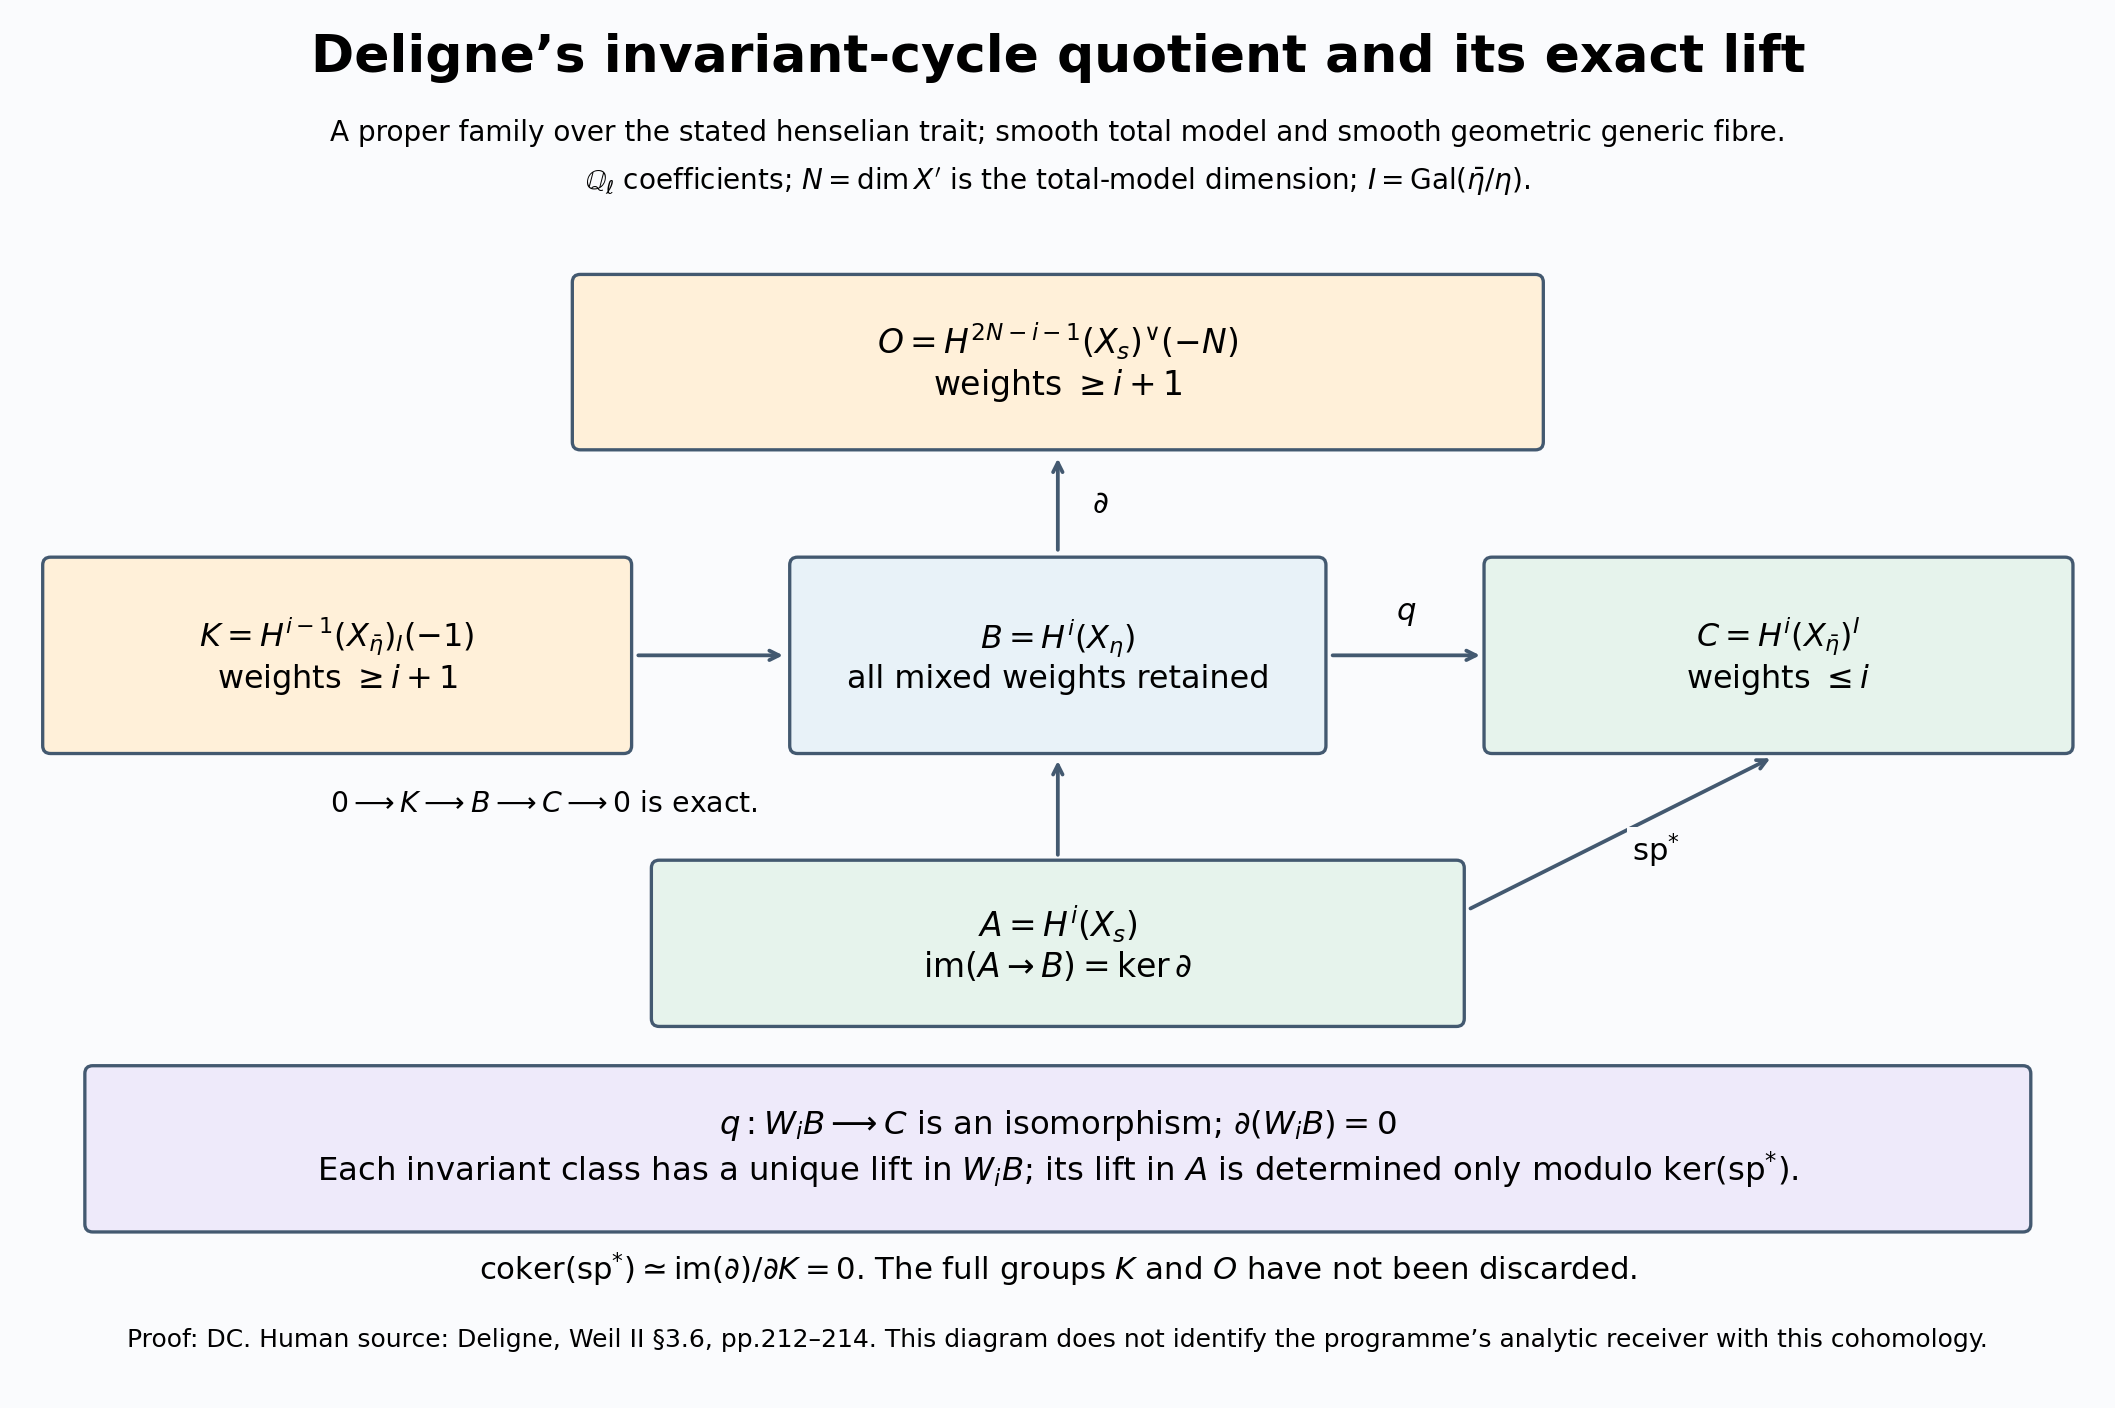
\includegraphics[keepaspectratio,alt={The invariant-cycle quotient and its exact lift}]{deligne_invariant_cycle_lift.png}}
\caption{The invariant-cycle quotient and its exact lift}
\end{figure}

The second diagram records the complete source quotient and obstruction.
DC proves the weight separation, the unique lift into the indicated
Frobenius weight part, and the full possible kernel of the lift into
special-fibre cohomology.

\begin{center}\rule{0.5\linewidth}{0.5pt}\end{center}

\chapter{Determinant weights and the complete tensor-power purity proof
---
DP0--DP9}\label{determinant-weights-and-the-complete-tensor-power-purity-proof-dp0dp9}

Proof source: \nolinkurl{DELIGNE_DETERMINANT_AND_TENSOR_PURITY.md}.

\chapter{Determinant weights, all tensor powers, and pointwise
purity}\label{determinant-weights-all-tensor-powers-and-pointwise-purity}

24 September 2026. Reconstruction DP0--DP9 of the determinant/tensor
purity mechanism in Pierre Deligne, \emph{La conjecture de Weil. II},
§§1.3--1.5. The dominant-pullback and étale-extension
assertions1.3.13(i),1.3.14--15 and the general nonsemisimple1.3.8 are
addressed in the separate monodromy-group supplement; they are not
claimed proved in this file. This derivation retains the source
arithmetic data. It does not assert that a new coefficient object on the
programme base has already been constructed.

\section{DP0. Source, conventions, and the exact
input}\label{dp0.-source-conventions-and-the-exact-input}

The entire current French transcription, printed pages137--252, was
read. The witness is
\nolinkurl{output/Deligne_Weil_II_S20_LaTeX/typed_latex/S20_FR_record_export.tex},
SHA256
\nolinkurl{d6836ae15d98f2b27eb98c9bd039a7d921679becd9fa47ff4717410289dbd351}.
It is a local transcription, not author TeX; the source-reading ledger
records its provenance and discrepancies. The passages reconstructed
here are printed pages156--165, §§1.3.1--1.5.3, together with
definitions1.1--1.2. No original PDF comparison is claimed.

Let \(q=p^f\), with \(p\ne\ell\) primes. Let \(X_0\) be a smooth
geometrically connected curve over \(\mathbb F_q\), and
\(X=X_0\times_{\mathbb F_q}\overline{\mathbb F}_q\). A geometric point
\(\bar x\) gives the exact Weil-group sequence \[
1\longrightarrow\pi_1(X,\bar x)\longrightarrow W(X_0,\bar x)
 \xrightarrow{\deg}\mathbb Z\longrightarrow0.
\tag{DP0.1}
\] The generator is \textbf{geometric} Frobenius. At a closed point
\(x\), set \(d_x=[k(x):\mathbb F_q]\) and \(N(x)=q^{d_x}\); \(F_x\) has
degree \(d_x\). These integers and fields are source data of Deligne's
theorem. They are not arithmetic placed on
\(\tau\langle Z_1;\text{no }Z_2\rangle\).

A lisse Weil sheaf \(\mathcal F_0\) is represented by a
finite-dimensional continuous representation of (DP0.1), defined over a
finite extension of \(\mathbb Q_\ell\) on the geometric subgroup. Fix
Deligne's coefficient embedding
\(\iota:\overline{\mathbb Q}_\ell\to\mathbb C\). For \(a\ne0\), write \[
w_{q}(a)=\frac{2\log|\iota a|}{\log q},\qquad
w_{N(x)}(a)=\frac{2\log|\iota a|}{d_x\log q}.
\tag{DP0.2}
\] These weights are logarithms of actual Frobenius eigenvalue moduli.
They are not distances between a support and a stalk. A Tate twist
\((r)\) multiplies \(F_x\) by \(N(x)^{-r}\), and subtracts \(2r\) from
its weight.

The established source inputs used below are global function-field class
field theory, the finite-field Picard variety, the representation theory
of reductive algebraic groups, Grothendieck's trace formula, and
Poincaré duality for curves. We give the deductions from these inputs,
including every weight and determinant step. We do not claim to reprove
the entire upstream SGA theory.

\section{DP1. Rank-one geometric monodromy and its exact
character}\label{dp1.-rank-one-geometric-monodromy-and-its-exact-character}

Let \(\chi:W(X_0,\bar x)\to E^\times\) be rank one, with
\(E/\mathbb Q_\ell\) finite. Deligne1.3.1 identifies the geometric part
of the abelianized Weil group, by class field theory, with degree-zero
idèle classes allowing ramification at the finite boundary
\(S=\overline X_0-X_0\). The map to the unramified degree-zero
divisor-class group has kernel a quotient of \[
\prod_{v\in S}\mathcal O_v^\times.
\tag{DP1.1}
\] Each local unit group has finite residue-unit quotient and pro-\(p\)
principal units. The unramified quotient is
\(\operatorname{Pic}^0(\overline X_0)(\mathbb F_q)\), a finite set
because the variety is of finite type over a finite field. Consequently
the geometric abelian image is finite-by-pro-\(p\).

The image of \(\pi_1(X,\bar x)\) under \(\chi\) is also compact in
\(E^\times\). Compactness makes its valuation image a finite subgroup of
\(\mathbb Z\), hence zero. It lies in \(\mathcal O_E^\times\), which has
an open pro-\(\ell\) subgroup. A group that is both pro-\(p\) and
pro-\(\ell\) is trivial when \(p\ne\ell\): every finite quotient has
order both a power of \(p\) and a power of \(\ell\). Taking the open
subgroups in the two descriptions therefore shows that the compact image
is finite.

Choose a positive integer \(h\) killing this finite image. Then
\(\chi^h\) is trivial on the kernel of degree, so \[
\chi(w)^h=b^{\deg w}
\tag{DP1.2}
\] for some \(b\ne0\). Choose \(c\) with \(c^h=b\), and put
\(\varepsilon(w)=\chi(w)c^{-\deg w}\). Direct substitution gives
\(\varepsilon(w)^h=1\). Thus \[
\boxed{\chi(w)=c^{\deg w}\varepsilon(w),\quad
\varepsilon^h=1,\quad
|\iota\chi(F_x)|=|\iota c|^{d_x}.}
\tag{DP1.3}
\] In particular rank one is pointwise \(\iota\)-pure of weight
\(w_q(c)\). No choice of an individual prime or closed point is used to
create the degree map; it is the full source sequence (DP0.1).

For an irreducible rank-\(n\) constituent \(\mathcal G_0\), apply
(DP1.3) to \(\det\mathcal G_0\). Its determinant weight is \[
\beta(\mathcal G_0)=\frac1n w_q(c_{\det\mathcal G_0}).
\tag{DP1.4}
\] If \(\alpha_1(x),\ldots,\alpha_n(x)\) are its eigenvalues with their
multiplicities, then \[
\sum_{j=1}^n w_{N(x)}(\alpha_j(x))=n\beta(\mathcal G_0)
\tag{DP1.5}
\] at \textbf{every} closed point. This is an equality about the product
of eigenvalues; individual equality has not yet been obtained.

The convention for a constant twist defined over \(\mathbb F_p\) is
important. If its Frobenius scalar is \(b\), it multiplies the
determinant at \(x\) by \[
b^{n[k(x):\mathbb F_p]}=b^{n f d_x}.
\tag{DP1.6}
\] This multiplication by \(f\), not division by \(f\), follows from the
degree of the residue-field extension. The available
transcription's1.3.6 exponent is inconsistent with1.2.7; equation(DP1.6)
derives the correction while retaining the original scalar and field.

\section{DP2. The central element that controls determinant
weights}\label{dp2.-the-central-element-that-controls-determinant-weights}

Replace \(\mathcal F_0\) by its semisimplification for this paragraph
only: determinants and constituent weights are unchanged, and no
extension is removed from later trace formulas. Let \(G^0\) be the
Zariski closure of geometric monodromy on its fibre. A degree-one lift
\(w\) normalizes \(G^0\). The group \[
G=G^0\rtimes_{\operatorname{Int}(\rho(w))}\mathbb Z
\tag{DP2.1}
\] receives the Weil group and all its tensor constructions. Its
identity component \(G^{00}\) is reductive. Indeed its unipotent radical
is characteristic in \(G^{00}\), hence normal in \(G\). The invariant
subspace in an irreducible \(G\)-module is nonzero by unipotence and
\(G\)-stable by normality, hence is the whole module. The radical
therefore acts trivially on the semisimple faithful fibre, and is
trivial.

We recall the rest of Deligne1.3.9's argument because reductivity alone
is insufficient. The connected central torus \(T_1\subset G^{00}\) acts
through a finite set of characters on the faithful fibre. These
characters generate its character group; conjugation permutes them, so
after a finite-index restriction conjugation acts trivially on \(T_1\).
The outer automorphisms of a reductive group that act trivially on its
connected centre form a finite group (the finite root-datum
automorphisms). A further finite-index restriction therefore makes the
degree action inner. After changing its lift by an element of
\(G^{00}\), this restriction is \(G^{00}\times\mathbb Z\). The
associated finite cover and constant-field extension retain a smooth
curve, and rank-one result(DP1.3) applies there.

The maximal torus quotient of \(G^{00}\) is isogenous to \(T_1\). Every
character of that quotient would give a rank-one Weil character with
finite geometric image by(DP1.3). Its geometric image is also Zariski
dense by construction. A finite subset cannot be Zariski dense in a
positive-dimensional torus. Therefore the torus quotient is trivial and
\(G^{00}\) is semisimple. Its centre is finite.

Choose a positive power of the degree-one lift \(w\) whose conjugation
is inner on \(G^{00}\) and trivial on the finite group \(G^0/G^{00}\).
Correct it by an element \(h_0\in G^{00}\), obtaining \(y=h_0w^m\) that
centralizes \(G^{00}\). For each representative \(h\) of \(G^0/G^{00}\),
the commutator \([y,h]\) lies in \(G^{00}\) because the component action
is trivial; it centralizes \(G^{00}\) because \(y\) does. Thus it lies
in the finite centre \(Z(G^{00})\). Also \([y,w]\) lies in \(G^{00}\),
by the expression \(y=h_0w^m\), and centralizes \(G^{00}\), so it lies
in that same finite centre. Since \(y\) centralizes this finite centre,
a common positive power kills all these commutators. That power
centralizes \(G^{00}\), the representatives of \(G^0/G^{00}\), and
\(w\), which together generate \(G\). We obtain \[
z\in Z(G),\qquad m=\deg(z)>0.
\tag{DP2.2}
\] This proves finite \textbf{index}, not finiteness, of the image of
\(Z(G)\to\mathbb Z\). Its kernel is contained in the finite centre of
\(G^0\). The contradictory wording ``finite subgroup of Z'' in the
available1.3.10(iv) is not used.

On any irreducible \(G\)-module \(V\), the central element \(z\) is a
scalar \(u\) by Schur's lemma. The determinant character extends(DP1.3)
from the Weil group to \(G\): its \(h\)-th power is trivial on geometric
monodromy, hence on its Zariski closure \(G^0\). Writing \(g=g_0w^d\)
gives \(\chi(g)^h=b^d\); choosing \(c^h=b\) yields
\(\varepsilon(g)=\chi(g)c^{-d}\) with \(\varepsilon(g)^h=1\). Thus
evaluation at \(z\), whether or not it is itself in the Weil-group
image, is legitimate. If \(V\) has rank \(r\), this gives \[
u^r=c^{m}\varepsilon(z),\qquad
|\iota u|^r=|\iota c|^{m},\qquad
\boxed{|\iota u|=q^{m\beta(V)/2}.}
\tag{DP2.3}
\] This proves1.3.12's central-character criterion with the rank and
degree factors intact.

Tensor products multiply eigenvalues of \(z\). Thus their determinant
weights add. In an exterior power, a triangular basis for the action of
\(z\) shows that every eigenvalue is a product of the chosen number of
diagonal eigenvalues. If the constituent weight \(\gamma\) occurs in
total rank \(n(\gamma)\), the determinant weights of
\(\bigwedge^a\mathcal F_0\) are \[
\sum_\gamma a(\gamma)\gamma,
\quad 0\le a(\gamma)\le n(\gamma),\quad
\sum_\gamma a(\gamma)=a.
\tag{DP2.4}
\] For nonsplit sheaves, a composition filtration induces the tensor and
exterior filtrations, and the same eigenvalue products give the weights
of their graded constituents. Hence these conclusions do not require
splitting extensions in the original sheaf.

\section{DP3. The complete curve trace identity and its
poles}\label{dp3.-the-complete-curve-trace-identity-and-its-poles}

For any lisse sheaf \(\mathcal V_0\) on the curve, write \(V\) for its
geometric fibre and \(\Pi=\pi_1(X,\bar x)\). The complete formulas are
\[
H^0(X,\mathcal V)=V^\Pi,
\quad
H_c^0(X,\mathcal V)=
\begin{cases}V^\Pi,&X\text{ proper},\\0,&X\text{ not proper},\end{cases}
\quad
H_c^2(X,\mathcal V)=V_\Pi(-1).
\tag{DP3.1}
\] The last equality follows from Poincaré duality with
\(H^0(X,\mathcal V^\vee(1))\); in particular the \((-1)\) and the
resulting factor \(q\) are retained. These invariant and coinvariant
spaces come from geometric-constant subobjects or quotients. If every
determinant weight of \(\mathcal V_0\) is at most \(b\), eigenvalues on
\(H_c^0\) have weight at most \(b\), and those on \(H_c^2\) have weight
at most \(b+2\).

Grothendieck's trace formula, Deligne1.4.5, gives \[
L(\mathcal V_0,t)
=\prod_{x\in|X_0|}\det(1-F_x t^{d_x}\mid\mathcal V_{\bar x})^{-1}
=\frac{\det(1-Ft\mid H_c^1(X,\mathcal V))}
{\det(1-Ft\mid H_c^0(X,\mathcal V))
 \det(1-Ft\mid H_c^2(X,\mathcal V))}.
\tag{DP3.2}
\] This begins as a formal series identity. For each coefficient only
finitely many closed points contribute. Every cohomology group, sign,
and multiplicity remains in(DP3.2). On an affine smooth connected curve,
\(H_c^0=0\) by(DP3.1), so its determinant is exactly1; this is a proved
vanishing, not a discarded term.

When eigenvalue weights at closed points are at most \(b\) and dimension
is \(d\), the Euler product converges absolutely for \[
|t|<q^{-b/2-d}.
\tag{DP3.3}
\] Indeed a finite decomposition into quasi-finite maps to affine space
bounds the number of degree-\(n\) closed points by \(Cq^{dn}\). The
absolute logarithmic expansion is bounded by a constant times
\(\sum_{n\ge1}q^{dn}q^{nb/2}|t|^n\), after summing repetitions
geometrically on a smaller closed disc. This converges. This argument is
Deligne1.4.6; it records how arithmetic point counts enter the analytic
function.

\section{DP4. Even tensor powers give positive coefficients, without a
positive
form}\label{dp4.-even-tensor-powers-give-positive-coefficients-without-a-positive-form}

All local and global L-functions in DP4--DP5 are complex series after
coefficientwise application of \(\iota\). This includes the determinant
on the left of(DP4.1).

Suppose that \(\mathcal F_0\) is \(\iota\)-real: the local polynomial
\(\iota\det(1-F_x u\mid\mathcal F_{\bar x})\) has real coefficients at
every closed point. Newton identities show that
\(\iota\operatorname{Tr}(F_x^j\mid\mathcal F_{\bar x})\) is real for
each \(j\ge1\). For a positive integer \(k\), set
\(\mathcal V_0=\mathcal F_0^{\otimes 2k}\). The exact local logarithm is
\[
\log\det(1-F_x t^{d_x}\mid\mathcal V_{\bar x})^{-1}
=\sum_{j\ge1}\frac{
 \bigl(\iota\operatorname{Tr}(F_x^j\mid\mathcal F_{\bar x})\bigr)^{2k}}
 {j}\,t^{j d_x}.
\tag{DP4.1}
\] The trace identity used here is
\(\operatorname{Tr}(A^{\otimes 2k})=(\operatorname{Tr}A)^{2k}\), proved
by multiplying diagonal entries in a tensor basis. Every coefficient on
the right is nonnegative. Exponentiating a series with nonnegative
coefficients and zero constant term gives nonnegative coefficients and
constant term1, because each coefficient of \(\sum_{r\ge0}h^r/r!\) is a
sum of nonnegative products.

Consequently each local factor \(L_{x,k}(t)\) has nonnegative Taylor
coefficients. The product of all other factors also has nonnegative
coefficients and constant term1. Coefficientwise, \[
0\le[t^n]L_{x,k}(t)\le[t^n]L(\mathcal F_0^{\otimes2k},t).
\tag{DP4.2}
\] For any finite \(n\), the assertion follows from the finite product
of points of degree at most \(n\), so there is no convergence assumption
hidden in this formal inequality.

This is positivity of power-series coefficients obtained from
\textbf{real traces at every closed point and every repetition}. No
positive inner product on the sheaf has been assumed, and no
reflection-positivity assertion about the programme has been inserted.

\section{DP5. Pole control implies each eigenvalue
inequality}\label{dp5.-pole-control-implies-each-eigenvalue-inequality}

For the zero sheaf there are no eigenvalues or constituents, so the
assertions are vacuous. Assume the sheaf has positive rank before taking
a largest determinant weight.

Let \(r\) be the largest determinant weight of \(\mathcal F_0\).
By(DP2.4), every constituent of \(\mathcal F_0^{\otimes2k}\) has
determinant weight at most \(2kr\). Remove a closed point different from
the particular point \(x\) being tested, making the curve affine. The
restriction retains the local eigenvalues at \(x\) and its determinant
weights: the fundamental group of the nonempty open curve surjects onto
that of the original normal curve, so constituents stay irreducible with
the same determinant characters.

Equations(DP3.1--2) show that the global rational function has no pole
in \[
|t|<R_k,\qquad R_k=q^{-(2kr+2)/2}.
\tag{DP5.1}
\] This uses the full possible \(H_c^2\) denominator. Cancellation with
the numerator can only remove poles, so it cannot invalidate the
asserted disc. The Taylor series of this rational function converges at
every \(0\le t<R_k\). Equation(DP4.2) and nonnegativity then make the
local factor's Taylor series converge there too. It therefore has radius
at least \(R_k\).

If \(\alpha\) is any eigenvalue of \(F_x\) on \(\mathcal F_{\bar x}\),
then \(\alpha^{2k}\) is an eigenvalue on the tensor power, including its
multiplicity. The reciprocal local determinant has a pole at every
solution of \[
t^{d_x}=(\iota\alpha)^{-2k},
\quad\text{each of modulus }|\iota\alpha|^{-2k/d_x}.
\tag{DP5.2}
\] Its numerator is1, so these poles cannot be cancelled locally. Radius
at least \(R_k\) implies \[
|\iota\alpha|^{2k/d_x}\le q^{(2kr+2)/2},
\qquad
w_{N(x)}(\alpha)\le r+\frac1k.
\tag{DP5.3}
\] The same fixed eigenvalue satisfies(DP5.3) for every positive integer
\(k\). If its weight exceeded \(r\) by \(e>0\), an integer \(k>1/e\)
would contradict(DP5.3). Thus \[
\boxed{w_{N(x)}(\alpha)\le r.}
\tag{DP5.4}
\] This is Deligne1.5.2 with the analytic coefficient-domination step
supplied in full. It uses all tensor powers to obtain an exact
conclusion, not a finite numerical sample.

\section{DP6. Exterior powers and determinant equality force every
constituent to be
pure}\label{dp6.-exterior-powers-and-determinant-equality-force-every-constituent-to-be-pure}

For each determinant weight \(\beta\), let \(n(\beta)\) be the total
rank of the corresponding constituents, and \(\alpha_i^\beta\),
\(1\le i\le n(\beta)\), their local eigenvalues at a fixed \(x\),
counted with multiplicity. From(DP1.5), \[
\sum_i w_{N(x)}(\alpha_i^\gamma)=n(\gamma)\gamma
\quad\text{for every }\gamma.
\tag{DP6.1}
\] Fix an occurring \(\beta\), and put
\(N_\beta=\sum_{\gamma>\beta}n(\gamma)\). The largest determinant weight
of \(\bigwedge^{N_\beta+1}\mathcal F_0\) is \[
r_\beta=\beta+\sum_{\gamma>\beta}n(\gamma)\gamma
\tag{DP6.2}
\] by(DP2.4): choose every higher-weight eigenvalue, then one at weight
\(\beta\). Exterior powers preserve the reality of the characteristic
polynomial because their eigenvalues are products and complex
conjugation permutes the original eigenvalue multiset. Hence DP5 applies
to this exterior power. Its eigenvalue \[
\alpha_i^\beta\prod_{\gamma>\beta}\prod_j\alpha_j^\gamma
\tag{DP6.3}
\] has weight at most \(r_\beta\). Subtract the equalities(DP6.1) for
\(\gamma>\beta\). This gives \(w_{N(x)}(\alpha_i^\beta)\le\beta\) for
each \(i\). Their sum is exactly \(n(\beta)\beta\) by(DP6.1). If any
individual inequality were strict, this sum would be strictly smaller.
Therefore \[
\boxed{w_{N(x)}(\alpha_i^\beta)=\beta
\quad\text{for every }x,\beta,i.}
\tag{DP6.4}
\] This completes the deduction of Deligne1.5.1. No chosen eigenvalue or
constituent has been dropped.

\section{DP7. The full real companion and its retained
scalar}\label{dp7.-the-full-real-companion-and-its-retained-scalar}

For a pointwise pure sheaf of integer weight \(n\), the source real
companion is \[
\mathcal F_0\oplus\mathcal F_0^\vee(-n).
\tag{DP7.1}
\] At \(x\), an eigenvalue \(a\) is paired with \(N(x)^n/a\). Since
\(|\iota a|^2=N(x)^n\), that second complex eigenvalue equals
\(\overline{\iota a}\). This proves reality and preserves the same
weight; the Tate factor is essential.

For arbitrary real \(\beta\) in the category of Weil sheaves, let
\(\mathcal L_{\beta}\) be the constant Weil line whose geometric
\(\mathbb F_q\)-Frobenius is the scalar \(\iota^{-1}(q^\beta)\). Its
value at \(x\) is \(N(x)^\beta\), and its weight is \(2\beta\). Then the
exact companion is \[
\mathcal F_0\oplus(\mathcal F_0^\vee\otimes\mathcal L_\beta).
\tag{DP7.2}
\] The proof is the same equality \(N(x)^\beta/a=\overline a\) after
\(\iota\). The scalar need not be an \(\ell\)-adic unit, which is why
Weil sheaves, rather than only étale sheaves, occur here. This
construction starts with proved pointwise purity; it is not an argument
establishing purity of an arbitrary sheaf merely by adjoining a dual.

\section{DP8. What this calculation actually supplies to weight
control}\label{dp8.-what-this-calculation-actually-supplies-to-weight-control}

The proved chain is: \[
\begin{gathered}
\text{rank-one geometric finiteness}
\longrightarrow\text{determinant weights and tensor rules}\\
\longrightarrow\text{all-even-power coefficient positivity}
\longrightarrow\text{global pole control}\\
\longrightarrow\text{pointwise constituent purity}.
\end{gathered}
\tag{DP8.1}
\] Every arrow has been calculated above. The curve's \(H_c^2\) Tate
twist supplies the \(+2\); all powers make its contribution \(1/k\), and
the exact determinant sum supplies equality. This is one genuine
weight-control mechanism. The later source proof uses the local
monodromy filtration and a Lefschetz pencil to pass from pointwise sheaf
purity to cohomological purity. Those steps have their own complete
reconstructions;(DP8.1) does not replace them.

\section{DP9. Named external inputs and reading
limits}\label{dp9.-named-external-inputs-and-reading-limits}

The rank-one argument uses Deligne1.3.1's explicitly cited global
class-field isomorphism and the Picard variety. The central-element
argument uses the root-datum description of automorphisms of a connected
reductive group cited in1.3.10. The cohomological trace identity and
duality are the theorems recalled in1.4.1--1.4.5. Their exact statements
used here are displayed, and the ensuing deductions are proved. A
complete reconstruction of the weight argument does not mean that these
foundational theories have all been independently rebuilt. The wider
full-source reading is recorded in
\nolinkurl{DELIGNE_FULL_READING_LOG.md}.

\begin{center}\rule{0.5\linewidth}{0.5pt}\end{center}

\chapter{Monodromy groups, dominant pullback, and the étale criterion
---
DMG0--DMG7}\label{monodromy-groups-dominant-pullback-and-the-uxe9tale-criterion-dmg0dmg7}

Proof source: \nolinkurl{DELIGNE_MONODROMY_GROUP_SUPPLEMENT.md}.

\chapter{Deligne's monodromy groups: dominant pullback, the radical, and
extension to étale
sheaves}\label{delignes-monodromy-groups-dominant-pullback-the-radical-and-extension-to-uxe9tale-sheaves}

Independent derivation, 24 September 2026. Labels DMG0--DMG7. This
supplement supplies the remaining group-theoretic arguments in Weil II
§1.3 requested after review of DP0--DP9. It does not modify the DP
reconstruction or construct coefficient objects on
\texttt{τ〈Z1;\ no\ Z2〉}.

\section{DMG0. Source and exact
dependencies}\label{dmg0.-source-and-exact-dependencies}

The source is Pierre Deligne, \emph{La conjecture de Weil. II}, IHÉS 52
(1980), 137--252. Read for this supplement: the entire current French
§1.3, printed pages 156--162, including the general rank-one variant on
page 158, propositions (1.3.8), (1.3.13), (1.3.14), and lemma (1.3.15).
The actual witness is

\texttt{S20\_FR\_record\_export.tex},

SHA256
\nolinkurl{d6836ae15d98f2b27eb98c9bd039a7d921679becd9fa47ff4717410289dbd351}.
This is the current page-record transcription, not author TeX. No PDF
was consulted. Source lines 560--746 contain the relevant discussion,
with the final paragraph of (1.3.15) at the start of printed page 162.
The available transcription says ``finite subgroup of Z'' in
(1.3.10)(iv); the proof, corollary (1.3.11), and the direct derivation
below give \textbf{finite index} instead. The witness is retained
unchanged.

Foundational inputs are stated explicitly: global function-field class
field theory and the Picard variety for rank one on curves; the
curve-joining and Frobenius-density facts used in the source's Katz
variant for general normal schemes; elementary theory of algebraic
groups in characteristic zero, including their radicals and central
isogenies; normality and the generic-point description of finite étale
covers; and local analytic exponential/logarithm for linear algebraic
groups over a finite extension of \texttt{Q\_ℓ}. The deductions required
here are proved below.

Fix \texttt{q=p\^{}f}, \texttt{p≠ℓ}. A connected normal finite-type
\texttt{F\_q} scheme is integral. Its field of global constants can be
larger than \texttt{F\_q}; write it as \texttt{F\_\{q\^{}\{d\_X\}\}}.
Geometric Frobenius over that field has degree \texttt{d\_X} relative to
\texttt{q}. We retain these constant-field degrees when comparing two
schemes.

For a Weil representation \texttt{V} on a geometrically connected base
with finite constant field of cardinality \texttt{Q}, its algebraic
monodromy extension is

\[
1\longrightarrow G^0\longrightarrow G\xrightarrow{\deg_Q}\mathbf Z\longrightarrow0.
\tag{DMG0.1}
\]

Here \texttt{G\^{}0} is the Zariski closure of geometric monodromy. A
chosen degree-one lift \texttt{w} gives \texttt{G=G\^{}0⋊w\^{}Z}; the
action is conjugation by its actual representation matrix. The identity
component of \texttt{G\^{}0} is denoted \texttt{G\^{}\{00\}}. The
superscript \texttt{0} in this source notation does not by itself mean
connected. The map \texttt{G→GL(V)} is faithful on \texttt{G\^{}0}, but
need not be faithful on all of \texttt{G}.

The determinant weight of an irreducible rank-\texttt{r} module is
\texttt{β=(1/r)w\_Q(c)}, where the determinant character is
\texttt{c\^{}\{deg\_Q\}ε}, \texttt{ε} finite order, and

\[
w_Q(c)=2\log_Q|\iota c|.
\]

\section{DMG1. The rank-one input on a general normal
base}\label{dmg1.-the-rank-one-input-on-a-general-normal-base}

\textbf{Source:} the variant following (1.3.4), printed page 158; the
curve proof is (1.3.1)--(1.3.4), printed pages 156--158.

For a smooth geometrically connected curve, class field theory
identifies the geometric part of the abelianized Weil group with the
degree-zero idèle-class group allowing ramification at the finite
boundary. Its quotient by the local boundary-unit groups is the rational
point group of \texttt{Pic\^{}0} over the finite constant field and is
finite. Each boundary-unit group has finite residue quotient and
pro-\texttt{p} principal units. Therefore this geometric abelian group
has an open pro-\texttt{p} subgroup.

The image of a rank-one \texttt{ℓ}-adic character lies in
\texttt{E\^{}×} for some finite extension \texttt{E/Q\_ℓ} and is compact
on the geometric fundamental group. Its valuation image is a finite
subgroup of \texttt{Z}, hence zero, so it lies in \texttt{O\_E\^{}×},
which has an open pro-\texttt{ℓ} subgroup. The intersection of the two
open descriptions is both pro-\texttt{p} and pro-\texttt{ℓ}, hence
trivial. The geometric image is finite.

Here is the general-base reduction used by the source. Let \texttt{X\_0}
be normal and connected, and let \texttt{χ} be a rank-one Weil character
with values in \texttt{E\^{}×}. Let \texttt{M} be the finite group of
roots of unity in \texttt{E}. For closed points \texttt{x,y}, the
curve-joining fact used by Deligne and Katz gives a curve comparison on
which the preceding result applies. It yields

\[
\chi(F_x)^{\deg(y)}\chi(F_y)^{-\deg(x)}\in M,
\tag{DMG1.1}
\]

or equivalently equality of \texttt{χ(F\_x)\^{}\{1/deg\ x\}} and
\texttt{χ(F\_y)\^{}\{1/deg\ y\}} in \texttt{E\^{}×⊗\_Z\ Q}, written
multiplicatively. Degrees here are relative to the same finite constant
field, so all ratios have been retained.

For a degree-zero closed-point cycle \texttt{∑\_x\ n\_x\ x}, equation
(DMG1.1) implies

\[
\chi\left(\prod_xF_x^{n_x}\right)\in M,
\qquad \sum_x n_x\deg(x)=0.
\tag{DMG1.2}
\]

The product is used only after applying the abelian character; no
noncommuting Frobenius representatives are identified. The
Frobenius-density statement used in the source says that these
degree-zero products are dense in the geometric abelian image. By
continuity and finiteness of \texttt{M}, the entire geometric image of
\texttt{χ} lies in \texttt{M}.

Choose \texttt{h≥1} killing that image. Then

\[
\chi(g)^h=b^{\deg_Q g},\qquad c^h=b,\qquad
\chi(g)=c^{\deg_Qg}\varepsilon(g),\quad\varepsilon^h=1.
\tag{DMG1.3}
\]

This is the rank-one input for arbitrary normal bases used in the group
arguments below. The general curve-joining and Frobenius-density inputs
are part of this deduction's scope; the curve case requires neither
additional input.

\section{DMG2. Semisimple input, connected reductivity, and the
finite-degree central
element}\label{dmg2.-semisimple-input-connected-reductivity-and-the-finite-degree-central-element}

\textbf{Source:} (1.3.9)--(1.3.12), printed pages 159--161. This also
records the repaired disconnected-group step needed in DP2.

Suppose the Weil representation \texttt{V} is semisimple. The unipotent
radical \texttt{U} of \texttt{G\^{}\{00\}} is characteristic in
\texttt{G\^{}\{00\}}, hence normal in \texttt{G}. In an irreducible
\texttt{G}-constituent, the \texttt{U}-invariant subspace is nonzero
because a unipotent group has a nonzero fixed vector. Normality makes
that invariant subspace \texttt{G}-stable, so it is the entire
constituent. Thus \texttt{U} acts trivially on \texttt{V}. Faithfulness
on \texttt{G\^{}0} gives \texttt{U=1}, proving that \texttt{G\^{}\{00\}}
is reductive.

Let \texttt{T\_1} be its connected central torus. The finitely many
characters by which \texttt{T\_1} acts on \texttt{V} generate its
character group, because the action is faithful. Conjugation by
\texttt{G} permutes these characters. A finite-index subgroup
consequently acts trivially on \texttt{T\_1}. The outer automorphisms of
a connected reductive group that act trivially on the connected centre
form a finite group: after fixing a pinning, the remaining action is
through the finite root datum. A further finite-index restriction makes
the degree action on \texttt{G\^{}\{00\}} inner. Remove the finite
geometric component group and correct the degree lift by an element of
\texttt{G\^{}\{00\}}. This yields a finite-index subgroup
\texttt{G\^{}\{00\}×Z}.

The corresponding finite étale cover and finite extension of the
constant field have geometric monodromy Zariski dense in
\texttt{G\^{}\{00\}}. Let \texttt{T} be the maximal torus quotient of
\texttt{G\^{}\{00\}}, which is isogenous to \texttt{T\_1}. A character
of \texttt{T}, extended trivially over the degree factor, gives a
rank-one Weil character. Its geometric image is finite by DMG1 and
Zariski dense in the character image of \texttt{T}. A
positive-dimensional torus cannot have a finite dense subset. Thus
\texttt{T=1}, so \texttt{G\^{}\{00\}} is semisimple and
\texttt{Z(G\^{}\{00\})} is finite.

Now derive a central element in the \textbf{original} \texttt{G}, rather
than merely in the finite-index subgroup. Write \texttt{H=G\^{}\{00\}}
and choose an original positive-degree lift \texttt{w}. Take a power
\texttt{w\^{}m} whose action on \texttt{H} is inner and whose induced
action on the finite group \texttt{G\^{}0/H} is trivial. Choose
\texttt{h\_0∈H} with
\texttt{Int(w\^{}m)\textbar{}\_H=Int(h\_0)\textbar{}\_H}, and set

\[
y=h_0^{-1}w^m.
\tag{DMG2.1}
\]

Then \texttt{y} centralizes \texttt{H} and acts trivially on
\texttt{G\^{}0/H}. If \texttt{a} is a representative of a component of
\texttt{G\^{}0},

\[
[y,a]\in H
\quad\text{and}\quad
\operatorname{Int}([y,a])|_H=1,
\]

so \texttt{{[}y,a{]}∈Z(H)}. Also \texttt{{[}y,w{]}∈H}: this follows
directly from \texttt{y=h\_0\^{}\{-1\}w\^{}m}. The same conjugation
calculation gives \texttt{{[}y,w{]}∈Z(H)}. The element \texttt{y}
centralizes these commutators. Let \texttt{e≥1} be an exponent of the
finite group \texttt{Z(H)}. Then

\[
[y^e,a]=[y,a]^e=1,
\qquad [y^e,w]=[y,w]^e=1.
\]

Together with its centralization of \texttt{H}, this proves

\[
z=y^e\in Z(G),\qquad \deg_Q z=em>0.
\tag{DMG2.2}
\]

The finite group here is \texttt{G\^{}0/G\^{}\{00\}}, not the infinite
group \texttt{G/G\^{}\{00\}}. The kernel of \texttt{deg\_Q:Z(G)→Z} is
finite: its intersection with \texttt{H} is contained in finite
\texttt{Z(H)}, and its image in \texttt{G\^{}0/H} is finite. Its
cokernel is finite by (DMG2.2).

For completeness, a rank-one relation such as (DMG1.3) extends from the
Weil group to all of \texttt{G}. Its restriction \texttt{χ\^{}h=1} on
geometric monodromy extends to \texttt{G\^{}0} by Zariski density. For
\texttt{g=g\_0w\^{}d}, this gives \texttt{χ(g)\^{}h=b\^{}d}. Therefore
\texttt{ε(g)=χ(g)c\^{}\{-d\}} is defined on \texttt{G} and satisfies
\texttt{ε\^{}h=1}, even when \texttt{g} is not the image of an actual
Weil element.

On an irreducible rank-\texttt{r} module, let \texttt{z} act by scalar
\texttt{u}, and put \texttt{m\_z=deg\_Q\ z}. Applying that extended
determinant relation gives

\[
u^r=c^{m_z}\varepsilon(z),\qquad
|\iota u|=Q^{m_z\beta/2}.
\tag{DMG2.3}
\]

The same criterion holds constituent by constituent for a general
finite-dimensional \texttt{G}-module. It is the precise scalar test used
below, including its degree and rank factors.

\section{DMG3. The full nonsplit radical
theorem}\label{dmg3.-the-full-nonsplit-radical-theorem}

\textbf{Source:} theorem (1.3.8) and its proof on printed page 160.

Let \texttt{V} now be any finite-dimensional Weil representation, with
no semisimplicity assumption. Choose a composition filtration

\[
0=V_0\subset V_1\subset\cdots\subset V_s=V,
\]

stable under the Weil group. The stabilizer \texttt{P⊂GL(V)} of this
filtration has the homomorphism

\[
\pi:P\longrightarrow\prod_{a=1}^sGL(V_a/V_{a-1}),
\tag{DMG3.1}
\]

whose kernel \texttt{U\_P} consists of matrices acting as the identity
on every graded quotient. In a basis adapted to the filtration, these
are block upper triangular with identity diagonal blocks; \texttt{U\_P}
is unipotent.

The original geometric closure \texttt{G\^{}0} lies in \texttt{P}. Let
\texttt{G\_1\^{}0} be the geometric closure on \texttt{Gr\ V}. Then

\[
\pi(G^0)=G_1^0,
\qquad
\ker(\pi|_{G^0})=G^0\cap U_P.
\tag{DMG3.2}
\]

For the equality of images, the algebraic group image is closed and
contains the dense geometric image defining \texttt{G\_1\^{}0};
conversely it is the image of the closure of that same geometric
monodromy. The kernel is unipotent because it is an algebraic subgroup
of \texttt{U\_P}.

The associated graded representation is semisimple, so DMG2 gives that
\texttt{(G\_1\^{}0)\^{}\{00\}} is semisimple. The map of identity
components

\[
G^{00}\twoheadrightarrow (G_1^0)^{00}
\tag{DMG3.3}
\]

is surjective. One way to verify this is that the image is a connected
normal closed subgroup, and the quotient of the target by it is an image
of the finite component group of \texttt{G\^{}0}; a connected finite
algebraic group in characteristic zero is trivial.

Let \texttt{R=Rad(G\^{}\{00\})}, the connected maximal solvable normal
subgroup. Its image under (DMG3.3) is connected, solvable, and normal in
a semisimple group, hence trivial. Consequently

\[
R\subseteq G^0\cap U_P.
\tag{DMG3.4}
\]

Every element of the latter group is unipotent, so \texttt{R} is
unipotent. This proves the entire assertion (1.3.8): the radical of the
connected geometric monodromy group is unipotent, including for nonsplit
extensions. The proof keeps the original filtration and its unipotent
kernel; it does not replace the original representation by its
semisimplification and then transfer an unproved conclusion back.

\section{DMG4. Dominant pullback gives a finite-index monodromy
comparison}\label{dmg4.-dominant-pullback-gives-a-finite-index-monodromy-comparison}

\textbf{Source:} the geometric group input for (1.3.13)(i), printed page
161.

Let \texttt{f:Y\_0→X\_0} be a dominant morphism between normal connected
finite-type schemes over \texttt{F\_q}. Let \texttt{K=k(X\_0)} and
\texttt{L=k(Y\_0)}. The algebraic closure of \texttt{K} inside the
finitely generated extension \texttt{L} is finite over \texttt{K}; its
separable part \texttt{K\_s} is also finite. After compatible geometric
generic points are chosen, restriction of absolute Galois groups has
image

\[
\operatorname{im}\bigl(\operatorname{Gal}(L^{sep}/L)\to
\operatorname{Gal}(K^{sep}/K)\bigr)
=\operatorname{Gal}(K^{sep}/K_s).
\tag{DMG4.1}
\]

The image is closed by compactness. Its fixed field inside
\texttt{K\^{}\{sep\}} is exactly \texttt{K\^{}\{sep\}∩L=K\_s}; Galois
correspondence then proves the displayed equality. Its index is
\texttt{{[}K\_s:K{]}}, retaining the finite extension rather than
declaring a surjection without qualification.

For a normal connected scheme, its generic-point Galois group surjects
onto the étale fundamental group: a connected finite étale cover is
normal and integral, and thus has connected generic fiber. The
commutative diagram of generic and scheme fundamental groups therefore
implies that

\[
H=\operatorname{im}(\pi_1(Y_0)\to\pi_1(X_0))
\]

is an open subgroup, of index at most \texttt{{[}K\_s:K{]}}. This is the
needed finite-index assertion; injectivity is neither stated nor used.

Let the exact constant fields be \texttt{F\_\{q\^{}\{d\_X\}\}} and
\texttt{F\_\{q\^{}\{d\_Y\}\}}. Dominance embeds the first in the second,
so \texttt{d\_X} divides \texttt{d\_Y}. Write \texttt{W\_q} for the
inverse image of \texttt{Z⊂\textbackslash{}widehat\ Z} using degree
relative to \texttt{F\_q}; its degree image for \texttt{X\_0} is
\texttt{d\_XZ}, and for \texttt{Y\_0} it is \texttt{d\_YZ}. The induced
map preserves that absolute degree. Thus

\[
\operatorname{im}(W_q(Y_0)\to W_q(X_0))=H\cap W_q(X_0).
\tag{DMG4.2}
\]

Indeed a lift in \texttt{π\_1(Y\_0)} of an element whose degree is an
integer already belongs to \texttt{W\_q(Y\_0)}. Conversely all Weil
elements have integer degree. The index is finite. Intersecting once
more with degree zero shows that the image of geometric \texttt{π\_1(Y)}
has finite index in geometric \texttt{π\_1(X)}.

For a representation \texttt{V} of \texttt{W\_q(X\_0)}, take the Zariski
closures of these geometric images on the \textbf{same} vector space.
The closure for \texttt{Y\_0} is an algebraic subgroup of finite index
in the closure for \texttt{X\_0}, so their identity components agree.
The monodromy extensions with retained absolute degree give an injective
comparison

\[
G_Y\hookrightarrow G_X
\tag{DMG4.3}
\]

onto a finite-index subgroup: injectivity follows because the map is the
identity inclusion on the geometric closure and preserves degree, and
finite index follows from the finite component quotient together with
\texttt{{[}d\_XZ:d\_YZ{]}=d\_Y/d\_X}. Choosing Weil lifts gives an
explicit semidirect-product description, but the subgroup and the
morphism do not depend on the chosen lifts.

\section{DMG5. Determinant weights are preserved and detected by
dominant
pullback}\label{dmg5.-determinant-weights-are-preserved-and-detected-by-dominant-pullback}

\textbf{Source:} proposition (1.3.13)(i), printed page 161.

The assertion is:

\[
V\text{ is purely of determinant weight }\beta
\quad\Longleftrightarrow\quad
f^*V\text{ is purely of determinant weight }\beta.
\tag{DMG5.1}
\]

For clarity, ``purely of determinant weight β'' means that \textbf{each
nonzero irreducible constituent} has determinant weight β. It is not yet
the assertion that every local eigenvalue has that weight.

First take \texttt{V} semisimple. Its restriction to a finite-index
subgroup is semisimple. To verify this, pass to a finite-index normal
core \texttt{H\_0}. The sum of simple \texttt{H\_0}-submodules of an
irreducible \texttt{W}-module is nonzero and \texttt{W}-stable, hence
the whole module. Thus restriction to \texttt{H\_0} is semisimple. For
an intermediate finite-index subgroup \texttt{H}, average an
\texttt{H\_0}-equivariant projection over the finite group
\texttt{H/H\_0}; characteristic zero permits division by its order. This
supplies invariant complements and proves semisimplicity for \texttt{H}
too.

Choose a central \texttt{z∈G\_X} of positive degree by DMG2. Some
positive power \texttt{z\^{}a} belongs to the finite-index subgroup
\texttt{G\_Y}. Let the absolute degree of \texttt{z} relative to
\texttt{q} be \texttt{m}. Then its degrees relative to the two exact
constant fields are

\[
\deg_{q^{d_X}}z=\frac{m}{d_X},\qquad
\deg_{q^{d_Y}}z^a=\frac{am}{d_Y}.
\tag{DMG5.2}
\]

Both displayed numbers are integers where used. On an irreducible
constituent of \texttt{V}, the element \texttt{z} acts by a scalar
\texttt{u}. If that constituent has determinant weight β, (DMG2.3) gives

\[
|\iota u|=(q^{d_X})^{(m/d_X)\beta/2}=q^{m\beta/2}.
\tag{DMG5.3}
\]

Every irreducible constituent of its restriction to \texttt{G\_Y}
inherits the scalar \texttt{u\^{}a} from \texttt{z\^{}a}. Applying the
same criterion over its exact constant field gives

\[
|\iota u^a|=q^{am\beta/2}
=(q^{d_Y})^{(am/d_Y)\beta/2}.
\tag{DMG5.4}
\]

Its determinant weight is therefore precisely β. Conversely, if all
restricted constituents have determinant weight β, choose a nonzero
restricted constituent inside each original irreducible constituent.
Equation (DMG5.4) then forces (DMG5.3), because
\texttt{a\textgreater{}0}; the original constituent has determinant
weight β.

For nonsplit \texttt{V}, its composition filtration pulls back to an
exact filtration. The multiset of constituents of \texttt{f\^{}*V} is
the union of the multisets obtained from its irreducible original
quotients. Replace those quotients, only for this constituent
calculation, by their direct sum; the semisimple argument just proved
applies. It proves (DMG5.1) for the original \texttt{V} without an
assertion that its extensions split.

The zero representation satisfies both sides vacuously for every β. No
maximum of an empty weight set is taken.

\section{DMG6. A compact Zariski-dense subgroup has compact normalizer
in a semisimple local
group}\label{dmg6.-a-compact-zariski-dense-subgroup-has-compact-normalizer-in-a-semisimple-local-group}

\textbf{Source:} lemma (1.3.15), printed pages 161--162. The proof here,
as in the source, treats characteristic zero.

Let \texttt{E/Q\_ℓ} be finite, let \texttt{H} be a connected semisimple
linear algebraic group over \texttt{E}, and let \texttt{K⊂H(E)} be
compact and Zariski dense. Then

\[
N_{H(E)}(K)=\{g\in H(E):gKg^{-1}=K\}
\]

is compact.

Choose a sufficiently small analytic neighborhood of the identity on
which exponential and logarithm are inverse. There is an open normal
subgroup \texttt{K\_0⊂K} contained in it: take the normal core in
\texttt{K} of a sufficiently small open subgroup. The finite group
\texttt{K/K\_0} has an exponent \texttt{n≥1}. For every \texttt{x∈K},
define

\[
\log_K(x)=\frac1n\log(x^n)\in\operatorname{Lie}H(E).
\tag{DMG6.1}
\]

This is independent of the sufficiently divisible exponent chosen. On an
analytic logarithm neighborhood, \texttt{log(y\^{}r)=r\ log\ y};
applying that identity after two chosen exponents have been replaced by
a common multiple proves independence. It is continuous on \texttt{K},
and commutes with conjugation wherever the conjugate also lies in a
compact subgroup. In particular its compact image is invariant under the
normalizer of \texttt{K}.

Let

\[
\mathfrak l=\operatorname{span}_E\log_K(K)\subseteq\operatorname{Lie}H.
\tag{DMG6.2}
\]

It is invariant under \texttt{Ad\ K}; the condition that a linear
subspace be preserved is Zariski closed, so density makes it
\texttt{Ad\ H}-invariant. Hence it is an ideal of the semisimple Lie
algebra. Such an ideal is the Lie algebra of a connected normal
algebraic subgroup \texttt{H\textquotesingle{}⊂H}: after extending to an
algebraic closure it is the sum of a set of simple ideals, hence of the
corresponding simple factors up to central isogeny; Galois stability
gives descent to \texttt{E}.

For the quotient map \texttt{π:H→H/H\textquotesingle{}}, logarithms
satisfy \texttt{log(π(x))=dπ(log(x))} near the identity. The right side
is zero for \texttt{x∈K} in a sufficiently small neighborhood. The
logarithm is injective there, so \texttt{π} kills an open subgroup of
\texttt{K}. Thus \texttt{π(K)} is finite. It is also Zariski dense in
the connected group \texttt{H/H\textquotesingle{}}. A finite closed
subset cannot be dense in a positive-dimensional connected algebraic
group. Therefore \texttt{H/H\textquotesingle{}=1} and

\[
\operatorname{span}_E\log_K(K)=\operatorname{Lie}H.
\tag{DMG6.3}
\]

Let \texttt{Λ} be the \texttt{O\_E}-span of this compact logarithm set.
It is bounded: choose an \texttt{E}-basis of \texttt{Lie\ H};
compactness bounds every coordinate of \texttt{log\_K(K)} by one finite
power of a uniformizer. Thus \texttt{Λ} lies in a fixed scalar multiple
of the standard lattice. Since \texttt{O\_E} is noetherian, it is
finitely generated; (DMG6.3) gives full rank. Therefore \texttt{Λ} is an
\texttt{O\_E}-lattice. Every element normalizing \texttt{K} preserves
\texttt{Λ} in both directions, so

\[
\operatorname{Ad}(N_{H(E)}(K))\subseteq GL_{O_E}(\Lambda).
\tag{DMG6.4}
\]

The group on the right is compact. The adjoint map has finite kernel and
factors as the finite central isogeny \texttt{H→H\_ad} followed by a
closed embedding in \texttt{GL(Lie\ H)}. Its inverse image of a compact
subset is compact. Here is a coordinate verification of that last
assertion. On affine coordinate rings, every chosen coordinate generator
\texttt{x\_j} of \texttt{E{[}H{]}} is integral over
\texttt{E{[}H\_ad{]}}, hence satisfies

\[
x_j^{r_j}+a_{j,r_j-1}x_j^{r_j-1}+\cdots+a_{j,0}=0,
\tag{DMG6.5}
\]

where each \texttt{a\_\{j,i\}} is a regular function on \texttt{H\_ad}.
On a compact set \texttt{C⊂H\_ad(E)}, put

\[
M_j=\max\left(1,\ \max_{0\le i<r_j}\sup_{c\in C}|a_{j,i}(c)|_E\right).
\tag{DMG6.6}
\]

If \texttt{\textbar{}x\_j\textbar{}\_E\textgreater{}M\_j}, the leading
term in (DMG6.5) strictly dominates every other term in the
nonarchimedean absolute value, which is impossible. Thus every
coordinate of every inverse-image point is bounded by the displayed
finite constant. The inverse image is closed and lies in a product of
compact balls in the local field; it is compact.

Take \texttt{C=H\_ad(E)∩GL\_\{O\_E\}(Λ)}, a closed subset of a compact
group. Equation (DMG6.4) puts the normalizer in its compact inverse
image. Finally the normalizer is closed: if \texttt{g\_a→g} with each
\texttt{g\_aKg\_a\^{}\{-1\}=K}, then for each \texttt{k∈K}, closedness
of \texttt{K} gives \texttt{gkg\^{}\{-1\}∈K}; applying the same argument
to inverses gives equality. A closed subset of the compact inverse image
is compact. This proves the lemma.

\section{DMG7. The determinant criterion for an irreducible Weil sheaf
to be
étale}\label{dmg7.-the-determinant-criterion-for-an-irreducible-weil-sheaf-to-be-uxe9tale}

\textbf{Source:} proposition (1.3.14), printed page 161, using (1.3.15).

Let \texttt{V} be an irreducible lisse Weil sheaf of rank \texttt{r} on
a normal connected finite-field scheme. Then

\[
V\text{ extends to an étale sheaf}
\quad\Longleftrightarrow\quad
\det V\text{ extends to an étale sheaf}.
\tag{DMG7.1}
\]

Necessity follows because exterior power is a continuous polynomial
operation on a continuous representation of the profinite fundamental
group. We prove sufficiency, retaining the scalar and degree.

Use the exact constant field of cardinality \texttt{Q=q\^{}\{d\_X\}} and
its degree. Let \texttt{G} be the monodromy extension, choose
\texttt{z∈Z(G)} of positive degree \texttt{m}, and let its action on
\texttt{V} be scalar \texttt{u}. Enlarge a finite coefficient field
\texttt{E/Q\_ℓ} so that the representation, the needed group equations,
and \texttt{z,u} are all defined over \texttt{E}. Suppose
\texttt{det\ V} is étale. Write its character using (DMG1.3) as
\texttt{χ=c\^{}\{deg\_Q\}ε}, with \texttt{ε\^{}h=1}. An étale character
has compact image on the profinite group, so \texttt{c} is an
\texttt{ℓ}-adic unit. The exact determinant equation at \texttt{z} is

\[
u^r=c^m\varepsilon(z).
\tag{DMG7.2}
\]

Applying the discrete valuation, for which roots of unity have valuation
zero, gives

\[
r\,v_E(u)=m\,v_E(c)=0.
\tag{DMG7.3}
\]

Hence \texttt{u} is a unit.

The subgroup

\[
G_1=G^{00}\,z^{\mathbf Z}\cong G^{00}\times z^{\mathbf Z}
\tag{DMG7.4}
\]

has finite index in \texttt{G}. The product is direct: \texttt{z} is
central, and a power of nonzero-degree \texttt{z} lies in
\texttt{G\^{}\{00\}} only when that power is zero. Let \texttt{W\_1} be
its inverse image in the Weil group, and let \texttt{W\_1\^{}0} be the
inverse image of \texttt{G\^{}\{00\}}. Projection in (DMG7.4) defines

\[
\rho:W_1\longrightarrow G^{00}(E).
\tag{DMG7.5}
\]

The subgroup \texttt{K=ρ(W\_1\^{}0)} is compact, because
\texttt{W\_1\^{}0} is a finite-index closed subgroup of geometric
\texttt{π\_1}, and it is Zariski dense in \texttt{G\^{}\{00\}} by the
definition of the monodromy closure and its identity component. Since
\texttt{W\_1\^{}0} is normal in \texttt{W\_1}, its image \texttt{K} is
normalized by \texttt{ρ(W\_1)}. DMG6 makes this normalizer compact. Thus
\texttt{ρ(W\_1)} is bounded.

For \texttt{w∈W\_1}, the full original representation is

\[
R(w)=\rho(w)\,u^{\deg_Q(w)/m}.
\tag{DMG7.6}
\]

The exponent is an integer. Since \texttt{u} is a unit, its positive and
negative powers lie in the compact group \texttt{O\_E\^{}×}. Both
factors in (DMG7.6) are bounded, so the image of \texttt{W\_1} is
bounded. The entire Weil group is a finite union of its cosets, so its
image is bounded as well.

Choose any lattice \texttt{L\_0⊂V\_E}. Boundedness gives an integer
\texttt{b≥0} such that \texttt{R(w)L\_0⊂π\_E\^{}\{-b\}L\_0} for all
\texttt{w}. Then

\[
L=\sum_w R(w)L_0
\tag{DMG7.7}
\]

is a full-rank \texttt{O\_E}-submodule between \texttt{L\_0} and
\texttt{π\_E\^{}\{-b\}L\_0}. It is finitely generated and hence a
lattice; the group action permutes its defining summands, so it is
stable. Thus the representation lands in the profinite group
\texttt{GL(L)}.

To see the extension explicitly, select a geometric Frobenius lift
\texttt{F} over the exact constant field. In the profinite arithmetic
fundamental group, the map from \texttt{Z} taking \texttt{1} to
\texttt{F} extends to a continuous map from
\texttt{\textbackslash{}widehat\ Z}, since the closure of the cyclic
group generated by one element in a profinite group is procyclic.
Composing with degree is the identity on
\texttt{\textbackslash{}widehat\ Z}, so this is a section. Hence

\[
\pi_1(X_0)=\pi_1(X)\rtimes\widehat{\mathbf Z},
\qquad W(X_0)=\pi_1(X)\rtimes\mathbf Z.
\tag{DMG7.8}
\]

Similarly the powers of \texttt{R(F)∈GL(L)} extend continuously from
\texttt{Z} to \texttt{\textbackslash{}widehat\ Z}. The compatibility of
the conjugation action with the already continuous geometric
representation holds for integer powers; density and continuity extend
it to \texttt{\textbackslash{}widehat\ Z}. Therefore

\[
R(\gamma F^a)=R(\gamma)R(F)^a,
\qquad \gamma\in\pi_1(X),\ a\in\widehat{\mathbf Z},
\tag{DMG7.9}
\]

defines the required continuous extension. Density makes it unique. This
proves sufficiency in (DMG7.1).

Finally every irreducible Weil sheaf is a retained constant twist of an
étale sheaf. Let \texttt{Q=p\^{}g} be the exact constant field and let
\texttt{c} be its determinant scalar in (DMG1.3). Choose

\[
b\in\overline{\mathbf Q}_\ell^\times,
\qquad b^{rg}=c^{-1}.
\tag{DMG7.10}
\]

Use the constant Weil line over \texttt{F\_p} on which its geometric
Frobenius acts by \texttt{b}. At a point of degree \texttt{d} over
\texttt{F\_Q}, this line acts by \texttt{b\^{}\{gd\}}. Twisting
\texttt{V} by it changes the determinant scalar from \texttt{c} to
\texttt{cb\^{}\{rg\}=1}, so the determinant character becomes exactly
the finite-order character \texttt{ε}. By (DMG7.1), the twisted sheaf
\texttt{V\_b} is étale. The original object is recovered by the exact
inverse twist

\[
V=V_b\otimes\mathcal L_{b^{-1}}.
\tag{DMG7.11}
\]

The determinant factor at a closed point is \texttt{b\^{}\{rgd\}}, not
\texttt{b\^{}\{rd/g\}}. No factor, scalar, degree, or extension class
has been suppressed. Equations (DMG7.10)--(DMG7.11) are a comparison
with the original sheaf, not a replacement of it in the weight
calculation.

\begin{center}\rule{0.5\linewidth}{0.5pt}\end{center}

\chapter{Local monodromy and mixed primitive weights ---
DLM1--DLM15}\label{local-monodromy-and-mixed-primitive-weights-dlm1dlm15}

Proof source: \nolinkurl{DELIGNE_LOCAL_MONODROMY_RECONSTRUCTION.md}.

\chapter{Deligne, Weil II §§1.6--1.9: local monodromy and exact weight
control}\label{deligne-weil-ii-1.61.9-local-monodromy-and-exact-weight-control}

Independent reconstruction, 24 September 2026. Result labels in this
file are DLM1--DLM15. This file reconstructs the specified part of
Deligne's argument; it does not assign a sheaf, Frobenius, nilpotent
operator, weight, distance, or vector to the programme's
\texttt{τ〈Z1;\ no\ Z2〉}.

\section{Source identity, reading coverage, and transcription
corrections}\label{source-identity-reading-coverage-and-transcription-corrections}

The work is Pierre Deligne, \emph{La conjecture de Weil. II},
Publications mathématiques de l'IHÉS \textbf{52} (1980), 137--252. The
source used here is the current French page-record export:

\texttt{S20\_FR\_record\_export.tex}

Its SHA256 is
\nolinkurl{d6836ae15d98f2b27eb98c9bd039a7d921679becd9fa47ff4717410289dbd351}.
It is a transcription with explicit page records, not author-supplied
TeX. The historical English math-mode file was used to compare ambiguous
formulas, not to override the French witness. No PDF was read for this
reconstruction.

Reading completed: every line of §§1.6--1.9, current export lines
874--1421, printed pages 165--181; the §1.9 heading begins on page 179.
Dependencies actually read: conventions (0.6)--(0.11), printed page 145;
§1.2, printed pages 153--155; §1.4, printed pages 162--163. The
reconstruction uses Grothendieck's trace formula, quasi-unipotence,
Abhyankar's lemma, and basic étale sheaf/cohomology results as the
external inputs identified by Deligne. It does not claim a new proof of
those foundations.

The witness is preserved unchanged. The following corrections are
independently forced by the formulas and definitions; they are not
accusations about Deligne's printed original:

\begin{enumerate}
\def\labelenumi{\arabic{enumi}.}
\tightlist
\item
  In (1.6.7), the exception in \texttt{Ne\_i=e\_\{i-2\}} must be
  \texttt{i≠−d}, with \texttt{Ne\_\{−d\}=0}; the witness writes
  \texttt{i≠d}.
\item
  In (1.6.13)'s uniqueness proof the witness contains the impossible
  inequality \texttt{k−2i−2≥k}. The necessary and true inequality is
  \texttt{k−2i−2≥2j−k} when \texttt{k≥i+1} and \texttt{j≤0}. DLM4 proves
  it with the arbitrary top weight retained.
\item
  In (1.6.14.3), both witnesses display a positive twist
  \texttt{(i+j)/2}. With the explicitly stated convention
  \texttt{N:V(1)→V}, the required formula is \[
  \operatorname{Gr}_i^M V\cong
  \bigoplus_{j\ge |i|,\ j\equiv i\ (2)}P_{-j}\left(-\frac{i+j}{2}\right).
  \tag{DLM-C1}
  \] Indeed \texttt{N\^{}r:Gr\_i\ V(r)→P\_\{−j\}} with
  \texttt{r=(i+j)/2} is the relevant isomorphism on the indicated
  summand. Its inverse supplies the negative twist. The witness's next
  assertion that both sides have equal weights independently requires
  this sign. DLM3 proves the formula, and DLM10 uses it without changing
  β.
\item
  In (1.7.5), the weight filtration is the \textbf{direct sum over
  \texttt{j≤i}} of generalized eigenspaces of weight \texttt{j}. The
  witness's \texttt{product\ over\ j\textless{}i} cannot have graded
  piece of weight \texttt{i}.
\item
  For geometric Frobenius \texttt{F} and \texttt{N:V(1)→V},
  \texttt{FNF\^{}\{-1\}=Q\^{}\{-1\}N}. Consequently the conjugation
  coefficient in the proof of (1.7.5), if
  \texttt{F\textquotesingle{}\textquotesingle{}\^{}n=exp(λN)F\textquotesingle{}\^{}n},
  is \texttt{μ=λ/(1−Q\^{}\{-n\})}. The witness displays
  \texttt{1−q\^{}n}. DLM6 includes the direct multiplication that checks
  this correction.
\item
  The denominator in (1.8.1.1) is \texttt{H\_c\^{}2}, as in the current
  French text. The historical English \texttt{H\^{}0} is not used. DLM8
  retains all three compact-support degrees before proving the
  degree-zero factor is 1 in the auxiliary affine curve.
\end{enumerate}

\section{DLM1. The monodromy filtration and its primitive
pieces}\label{dlm1.-the-monodromy-filtration-and-its-primitive-pieces}

\textbf{Source:} (1.6.1)--(1.6.7), printed pages 165--166.

Let \texttt{V} be an object of an abelian category and let
\texttt{N:V→V} be nilpotent. There is a unique finite increasing
filtration \texttt{M} satisfying

\[
NM_i\subseteq M_{i-2},\qquad
N^k:\operatorname{Gr}_k^M V\xrightarrow{\sim}\operatorname{Gr}_{-k}^M V
\quad(k\ge0).
\tag{DLM1.1}
\]

Here a finite filtration is exhaustive and zero in sufficiently low
degree. The subscript \texttt{0} is a filtration index. It is not a base
point of the scheme, nor the centre of a geometric circle.

\textbf{Existence and uniqueness.} Induct on an integer \texttt{d≥0} for
which \texttt{N\^{}\{d+1\}=0}. For \texttt{d=0}, the conditions force
\texttt{M\_\{−1\}=0,M\_0=V}. For \texttt{d\textgreater{}0}, the extreme
pieces must be

\[
M_d=V,\quad M_{d-1}=\ker N^d,\quad
M_{-d}=\operatorname{im}N^d,\quad M_{-d-1}=0.
\tag{DLM1.2}
\]

To see that they are forced, (DLM1.1) and \texttt{N\^{}\{d+1\}=0} imply
\texttt{Gr\_k=0} for \texttt{k\textgreater{}d}; symmetry gives the same
for \texttt{k\textless{}−d}. On the remaining top graded piece,
\texttt{N\^{}d} is an isomorphism to the bottom graded piece. Its kernel
in \texttt{V} is therefore \texttt{M\_\{d−1\}}, and its image is
\texttt{M\_\{−d\}}. On

\[
\ker N^d/\operatorname{im}N^d
\]

the induced \texttt{N\^{}d} is zero. Its monodromy filtration is already
constructed uniquely by induction. Pull its pieces back into
\texttt{ker\ N\^{}d}, and attach (DLM1.2). The lowering condition and
the isomorphisms follow on the middle graded pieces by induction and on
the extreme pieces from the image/coimage isomorphism for
\texttt{N\^{}d}. This proves both assertions.

Set

\[
P_i(V)=\ker\bigl(N:\operatorname{Gr}_i^M V\longrightarrow
\operatorname{Gr}_{i-2}^M V\bigr).
\tag{DLM1.3}
\]

For \texttt{i\textgreater{}0}, \texttt{N} is injective on
\texttt{Gr\_i}, because its composite with \texttt{N\^{}\{i−1\}} is the
isomorphism \texttt{N\^{}i}; hence \texttt{P\_i=0}. For \texttt{j≥0},
the composite

\[
\operatorname{Gr}_{j+2}^M V
\xrightarrow{N^{j+1}}\operatorname{Gr}_{-j}^M V
\xrightarrow{N}\operatorname{Gr}_{-j-2}^M V
\]

is an isomorphism. Therefore

\[
\operatorname{Gr}_{-j}^M V
=P_{-j}\oplus N^{j+1}\operatorname{Gr}_{j+2}^M V.
\tag{DLM1.4}
\]

Iterating this direct sum, then using \texttt{N\^{}i:Gr\_i→Gr\_\{−i\}},
yields, for a chosen actual endomorphism \texttt{N},

\[
\operatorname{Gr}_i^M V\cong
\bigoplus_{j\ge |i|,\ j\equiv i\ (2)}P_{-j}.
\tag{DLM1.5}
\]

The map \nolinkurl{N:(V,M)→(V,M shifted by 2)} is strict:

\[
N(M_{i+2})=\operatorname{im}N\cap M_i.
\tag{DLM1.6}
\]

If \texttt{i\textless{}0}, its associated graded onto \texttt{M\_i} is
surjective by (DLM1.5), and finite filtrations imply surjectivity. If
\texttt{i+2\textgreater{}0}, the induced map
\texttt{V/M\_\{i+2\}→V/M\_i} is injective on associated gradeds, hence
injective. These cases cover every integer \texttt{i}. Thus kernels
commute with passage to the associated graded:

\[
\operatorname{Gr}_i^M(\ker N)\cong P_i.
\tag{DLM1.7}
\]

For finite-dimensional vector spaces, a Jordan string of length
\texttt{d+1} has vectors

\[
e_d,e_{d-2},\ldots,e_{-d},\qquad
Ne_i=e_{i-2}\ (i> -d),\quad Ne_{-d}=0.
\]

Its filtration is \texttt{M\_i=span\{e\_j:j≤i\}}. Direct sums of these
strings give the entire filtration. The string's primitive vector is its
\textbf{lowest} vector \texttt{e\_\{−d\}}. This specifies the sign of
every primitive index above.

\section{DLM2. The SL(2) construction, tensor products, and
duals}\label{dlm2.-the-sl2-construction-tensor-products-and-duals}

\textbf{Source:} (1.6.8)--(1.6.12), printed pages 167--168.

Now work over a characteristic-zero field. On a string of length
\texttt{d+1}, put \texttt{e\_r=e\_\{−d+2r\}} for \texttt{0≤r≤d}. Define

\[
H e_r=(-d+2r)e_r,\qquad
F e_r=e_{r-1},\qquad
E e_r=(d-r)(r+1)e_{r+1},
\tag{DLM2.1}
\]

with the out-of-range vectors zero. Then \texttt{F=N}, and direct
substitution gives

\[
[H,E]=2E,\qquad[H,F]=-2F,\qquad[E,F]=H.
\]

This is the irreducible \texttt{SL(2)} representation
\texttt{S\_d=Sym\^{}d(k\^{}2)} in a rescaled basis. On the associated
graded, the grading itself prescribes \texttt{H}, and the primitive
decomposition prescribes these strings. Thus one obtains the
\texttt{SL(2)} representation of (1.6.10), with the diagonal matrix
\texttt{diag(λ,λ\^{}\{-1\})} acting by \texttt{λ\^{}i} on
\texttt{Gr\_i\^{}M\ V}. This representation is on the associated graded;
no choice of a splitting of \texttt{V} is being declared canonical.

For \texttt{(V\textquotesingle{},N\textquotesingle{})} and
\texttt{(V\textquotesingle{}\textquotesingle{},N\textquotesingle{}\textquotesingle{})},
use exactly

\[
V=V'\otimes V'',\qquad N=N'\otimes1+1\otimes N''.
\tag{DLM2.2}
\]

On the tensor product \texttt{SL(2)} representation, diagonal weights
add and the lowering generator is precisely (DLM2.2). Its increasing
weight filtration therefore satisfies (DLM1.1); uniqueness gives

\[
M_i(V'\otimes V'')=\sum_{a+b=i}M_aV'\otimes M_bV''.
\tag{DLM2.3}
\]

The dual operator is \texttt{−N\^{}t}, not \texttt{N\^{}t}:
differentiation of the contragredient action introduces the minus sign.
Diagonal weights negate, so

\[
M_i(V^*)=(M_{-i-1}V)^\perp.
\tag{DLM2.4}
\]

For finite filtrations, choosing splittings verifies the natural
isomorphisms

\[
\operatorname{Gr}(V'\otimes V'')\cong\operatorname{Gr}V'\otimes\operatorname{Gr}V'',
\qquad
\operatorname{Gr}_i(V^*)\cong(\operatorname{Gr}_{-i}V)^*;
\]

the maps themselves are induced by classes and pairings and do not
depend on the splittings used to verify bijectivity.

Choose a nonzero lowest-weight vector in each \texttt{S\_d}, and choose
the Clebsch--Gordan isomorphisms

\[
S_{d'}\otimes S_{d''}\cong
\bigoplus_{j\in P(d',d'')}S_j,
\quad
P(d',d'')=\{j:|d'-d''|\le j\le d'+d'',\ j\equiv d'+d''\pmod2\}.
\tag{DLM2.5}
\]

These decompositions follow by multiplying the characters
\texttt{z\^{}d+z\^{}\{d−2\}+⋯+z\^{}\{−d\}} and subtracting successively
the highest character. Every listed summand occurs once. Complete
reducibility in characteristic zero makes this a direct sum of
representations. The isomorphisms involve the stated choices; the source
does not assert a unique scalar for every Clebsch--Gordan component.

The lowest-weight inclusion gives

\[
\operatorname{Gr}^M V\cong\bigoplus_{j\ge0}S_j\otimes P_{-j},
\quad
P_{-j}\cong\operatorname{Hom}_{SL(2)}(S_j,\operatorname{Gr}^M V).
\tag{DLM2.6}
\]

Applying (DLM2.5) to (DLM2.6) gives the primitive tensor decomposition.
Twists must be restored when \texttt{N} belongs to a nontrivial line, as
follows.

\section{DLM3. The monodromy line and every Tate
twist}\label{dlm3.-the-monodromy-line-and-every-tate-twist}

\textbf{Source:} (1.6.14), printed pages 169--170.

Let \texttt{𝔑} be a one-dimensional vector space acting nilpotently on
\texttt{V}, and write \texttt{V(k)=V⊗𝔑\^{}\{⊗k\}}; negative \texttt{k}
uses the dual line. The action is a map \texttt{N:V(1)→V}. Choosing a
basis in \texttt{𝔑} turns it into an endomorphism. Changing that basis
multiplies the endomorphism by a nonzero scalar, leaving \texttt{M} and
\texttt{P\_i} unchanged. Iterated action is the basis-independent map

\[
N^k:\operatorname{Gr}_{a+k}^M\operatorname{Gr}_a^W V(k)
\longrightarrow\operatorname{Gr}_{a-k}^M\operatorname{Gr}_a^W V.
\tag{DLM3.1}
\]

The primitive decomposition, tensor primitive decomposition and dual
primitive decomposition are

\[
\operatorname{Gr}_i^M V\cong
\bigoplus_{j\ge|i|,\ j\equiv i\ (2)}P_{-j}\left(-\frac{i+j}{2}\right),
\tag{DLM3.2}
\]

\[
P_{-j}(V'\otimes V'')\cong
\bigoplus_{j\in P(j',j'')}
P_{-j'}(V')\otimes P_{-j''}(V'')
\left(\frac{j-j'-j''}{2}\right),
\tag{DLM3.3}
\]

\[
P_{-j}(V^*)\cong P_{-j}(V)^*(j).
\tag{DLM3.4}
\]

To check (DLM3.2), let \texttt{r=(i+j)/2}. The \texttt{j}-string in
degree \texttt{i} maps isomorphically to its lowest vector by
\texttt{N\^{}r} after tensoring the source with \texttt{𝔑\^{}\{⊗r\}}.
Solving for the source gives twist \texttt{−r}. To check (DLM3.3), the
component of length \texttt{j} arises from the two strings by
\texttt{r=(j\textquotesingle{}+j\textquotesingle{}\textquotesingle{}−j)/2}
contractions; under rescaling \texttt{N}, its comparison with the chosen
primitive vectors has exactly \texttt{r} inverse powers of the
monodromy-line basis. This gives twist \texttt{−r}. Equivalently, retain
the strings as \texttt{S\_j} with the monodromy-line grading: the
primitive degree \texttt{−j} is obtained from degree
\texttt{−j\textquotesingle{}−j\textquotesingle{}\textquotesingle{}} by
raising \texttt{2r}, and each raising contributes \texttt{𝔑\^{}\{-1\}}.
For the dual, the lowest vector comes from the dual of the highest
vector, which by (DLM3.2) is the dual of \texttt{P\_\{−j\}(-j)}; this is
\texttt{P\_\{−j\}\^{}*(j)}.

In the geometric application,
\texttt{𝔑=\textbackslash{}overline\{\textbackslash{}mathbf\ Q\}\_\textbackslash{}ell(1)},
geometric Frobenius acts on it by \texttt{Q\^{}\{-1\}}, and its weight
is \texttt{−2}. The weight checks on (DLM3.2)--(DLM3.4) are then
respectively

\[
-j-2\left(-\frac{i+j}{2}\right)=i,
\quad
-j'-j''-2\left(\frac{j-j'-j''}{2}\right)=-j,
\quad j-2j=-j.
\]

These checks do not replace the maps; they verify the twists in the maps
just constructed.

\section{DLM4. Uniqueness of relative monodromy, with arbitrary top
weight
retained}\label{dlm4.-uniqueness-of-relative-monodromy-with-arbitrary-top-weight-retained}

\textbf{Source:} (1.6.13), printed pages 168--169.

Let \texttt{W} be a finite increasing filtration on \texttt{V},
preserved by \texttt{N}. There is at most one finite increasing
\texttt{M} with

\[
NM_i\subseteq M_{i-2},\qquad
N^k:\operatorname{Gr}_{a+k}^M\operatorname{Gr}_a^W V
\xrightarrow{\sim}\operatorname{Gr}_{a-k}^M\operatorname{Gr}_a^W V
\quad(a\in\mathbf Z,\ k\ge0).
\tag{DLM4.1}
\]

This is a uniqueness assertion; existence for a mixed sheaf is proved in
DLM11 and DLM14, not inserted here as an assumption about arbitrary
filtered objects.

Induct on the length of \texttt{W}. Let \texttt{a} be its top nonzero
degree, so \texttt{W\_a=V}. The restriction to \texttt{W\_\{a−1\}} is
unique by induction; on \texttt{Gr\_a\^{}W\ V}, the filtration is the
absolute monodromy filtration centred at \texttt{a}. Let its range be
contained in \texttt{{[}a−c,a+c{]}}. For \texttt{r≥0}, a putative
filtration satisfies

\[
\begin{aligned}
M_{a-r}&=M_{a-r}(W_{a-1}) &&(r>c),\\
M_{a-r}&=M_{a-r}(W_{a-1})+N^rM_{a+r},\\
M_{a+r}&=\ker\left(N^{r+1}:V\longrightarrow V/M_{a-r-2}\right).
\end{aligned}
\tag{DLM4.2}
\]

The first formula says that the quotient has no degree that low. For the
second, the lowering condition gives inclusion of the right side into
the left, while the induced \texttt{N\^{}r} maps the quotient's
\texttt{M\_\{a+r\}} onto its \texttt{M\_\{a−r\}}, as one sees on each
string centred at \texttt{a}. For the third, one inclusion follows from
lowering. On \texttt{G=Gr\_j\^{}W\ V}, \texttt{j≤a}, the reverse
inclusion follows because

\[
N^{r+1}:G/M_{a+r}G\longrightarrow G/M_{a-r-2}G
\]

is injective. On a degree \texttt{k\textgreater{}a+r}, the central
isomorphism runs from \texttt{k} to \texttt{2j−k}. The shorter iterate
by \texttt{r+1} remains injective since

\[
k-2r-2\ge 2j-k,
\]

which follows from \texttt{k≥a+r+1} and \texttt{j≤a}. Passage to
\texttt{Gr\^{}W} of a kernel injects into the corresponding kernel;
finite filtrations then give the required inclusion in \texttt{V}.
Starting in sufficiently large \texttt{r} and descending, the three
formulas determine alternately \texttt{M\_\{a+r\}} and
\texttt{M\_\{a-r\}}. This proves uniqueness without replacing \texttt{a}
by zero.

\section{DLM5. Local inertia and its
logarithm}\label{dlm5.-local-inertia-and-its-logarithm}

\textbf{Source:} (1.7.1)--(1.7.3), printed pages 170--171.

Let \texttt{R} be a henselian discrete valuation ring, with fraction
field \texttt{K}, residue field \texttt{k}, and compatible algebraic
closures. The exact sequence and tame quotient are

\[
1\to I\to\operatorname{Gal}(\bar K/K)\to\operatorname{Gal}(\bar k/k)\to1,
\] \[
1\to P\to I\xrightarrow{t}\prod_{\ell'\ne p}\mathbf Z_{\ell'}(1)\to1.
\tag{DLM5.1}
\]

Here \texttt{p} is the residue characteristic exponent and \texttt{P} is
pro-\texttt{p}. Fix \texttt{ℓ≠p}; the \texttt{ℓ}-component is
\texttt{t\_ℓ:I→Z\_ℓ(1)}.

For a quasi-unipotent \texttt{ℓ}-adic representation \texttt{ρ} of
\texttt{I}, there is a unique nilpotent line action

\[
N:V(1)\longrightarrow V
\quad\text{with}\quad
\rho(\sigma)=\exp(Nt_\ell(\sigma))
\tag{DLM5.2}
\]

on a sufficiently small finite-index subgroup of \texttt{I}. The
exponential and logarithm are finite polynomials on nilpotent/unipotent
matrices. The prime-to-\texttt{ℓ} kernel cannot have a nontrivial image
in a sufficiently small torsion-free pro-\texttt{ℓ} unipotent group.
Thus this restriction factors through \texttt{Z\_ℓ(1)}. Taking the
logarithm and dividing by a nonzero element of an open subgroup
determines the unique linear action of \texttt{Q̄\_ℓ(1)}. This also shows
independence of the finite-index subgroup.

If \texttt{k} is finite with \texttt{Q} elements, the local Weil group
is the inverse image of the integer powers of geometric Frobenius. Its
representations satisfy quasi-unipotence, the theorem of Grothendieck
cited by Deligne. The Frobenius conjugation explains the finite-order
semisimple part: after removing the finite wild and prime-to-\texttt{ℓ}
images, a tame generator has its eigenvalue multiset preserved by the
\texttt{Q}-power map. Each eigenvalue consequently has finite
multiplicative order; a common positive power is unipotent. This is
compatible with (DLM5.2), whose coordinate-free \texttt{N} is
Weil-equivariant.

Choosing a basis for the Tate line displays that equivariance as

\[
FNF^{-1}=Q^{-1}N.
\tag{DLM5.3}
\]

The nilpotent operator is not an involution. Except for the zero
operator, a nilpotent operator cannot square to the identity. Its
exponential is the unipotent part of monodromy, and all its tensor and
dual operations have been specified above.

\section{DLM6. Independence of Frobenius lift and the local weight
filtration}\label{dlm6.-independence-of-frobenius-lift-and-the-local-weight-filtration}

\textbf{Source:} (1.7.4)--(1.7.7), printed pages 171--172.

If \texttt{F\textquotesingle{}} and
\texttt{F\textquotesingle{}\textquotesingle{}} are lifts of the same
residue Frobenius, their eigenvalues differ by roots of unity. One can
pass to semisimplification for this eigenvalue assertion. There the
inertia image is finite: an irreducible constituent's \texttt{ker\ N} is
nonzero and Weil-stable by (DLM5.3), so it is the whole constituent and
\texttt{N=0}. In a representation with finite inertia image, choose a
power of Frobenius that centralizes that finite image, then a further
power killing the finite discrepancy between the two lifts. The
resulting powers of \texttt{F\textquotesingle{}} and
\texttt{F\textquotesingle{}\textquotesingle{}} agree. Their eigenvalues
before powering therefore differ by roots of unity.

Thus

\[
w_Q(\alpha)=2\log_Q|\iota\alpha|
\]

is independent of the lift. Suppose these weights are integers. For a
chosen lift, let \texttt{V\_j\textquotesingle{}} be the sum of its
generalized eigenspaces of weight \texttt{j} and set

\[
M_i'=\bigoplus_{j\le i}V_j'.
\tag{DLM6.1}
\]

The operator \texttt{N} takes \texttt{V\_j\textquotesingle{}} to
\texttt{V\_\{j−2\}\textquotesingle{}} by (DLM5.3). For two lifts, choose
\texttt{n\textgreater{}0} for which their powers differ by unipotent
inertia:

\[
F''^n=\exp(\lambda N)F'^n.
\]

All powers of \texttt{N} commute. Direct multiplication gives

\[
\begin{aligned}
\exp(\mu N)F'^n\exp(-\mu N)
&=\exp(\mu N)\exp(-\mu Q^{-n}N)F'^n\\
&=\exp(\mu(1-Q^{-n})N)F'^n.
\end{aligned}
\tag{DLM6.2}
\]

Take \texttt{μ=λ/(1−Q\^{}\{−n\})}. Passing from
\texttt{F\textquotesingle{}} to \texttt{F\textquotesingle{}\^{}n} does
not change the partition into weights, because
\texttt{w\_\{Q\^{}n\}(α\^{}n)=w\_Q(α)}. The operator \texttt{exp(μN)}
preserves each \texttt{M\_i\textquotesingle{}}; therefore the
filtrations obtained from the two lifts coincide. Conjugating a lift by
any Weil-group element gives another lift, so \texttt{M} is Weil-stable.
Uniqueness follows from the decomposition into generalized eigenspaces:
a filtration with pure graded weights must place the generalized
weight-\texttt{j} summand in degree \texttt{j}.

In particular \texttt{NM\_i(1)⊂M\_\{i−2\}}. A locally pure
representation has a single weight, so \texttt{N=0} and inertia has
finite image. This does \textbf{not} say that the local representation
at the boundary of a pointwise pure sheaf is pure. DLM10 calculates its
several weights \texttt{β+i}; nonzero local monodromy is exactly
compatible with those shifts.

Without the integral-weight restriction, grouping eigenvalues modulo
\texttt{Q\^{}Z} times roots of unity gives the canonical decomposition
in (1.7.7). The same conjugation proof works: multiplication of an
eigenvalue by \texttt{Q\^{}\{-1\}} keeps its class, so \texttt{N}
preserves each class and the exponential comparisons preserve the
decomposition. Each class can be twisted by a rank-one character to
obtain integral weights. This last comparison retains the twisting
scalar; it is not a replacement of the original representation in DLM10.

\section{DLM7. The tame normal-crossing specialization functor and its
exact
compatibility}\label{dlm7.-the-tame-normal-crossing-specialization-functor-and-its-exact-compatibility}

\textbf{Source:} (1.7.8)--(1.7.12), printed pages 172--174.

Let \texttt{X} be regular, let \texttt{D=⋃\_\{i∈I\}D\_i} be a
normal-crossing divisor with smooth transverse components, and put
\texttt{E=⋂D\_i}. Locally choose equations \texttt{t\_i=0}. For
\texttt{n} invertible on \texttt{X}, form

\[
X_n=X[T_i:i\in I]/(T_i^n-t_i:i\in I).
\tag{DLM7.1}
\]

Over \texttt{X−D} this is an étale cover, with \texttt{μ\_n\^{}I} acting
by \texttt{T\_i↦r\_iT\_i}. Above \texttt{E} the reduced section is
\texttt{T\_i=0}. For a locally constant finite sheaf tamely ramified
through primes in \texttt{L}, Abhyankar's lemma supplies such an
\texttt{n} after which the pullback extends locally constantly over
\texttt{X\_n}. Restrict that extension to the section over \texttt{E};
its inherited \texttt{μ\_n\^{}I} action defines \texttt{𝓕{[}E{]}}.
Passing through compatible finite levels gives the \texttt{ℓ}-adic
construction and an action of

\[
\mathbf Z_L(1)^I=\left(\prod_{\ell'\in L}\mathbf Z_{\ell'}(1)\right)^I.
\]

This functor is exact on the stated locally constant sheaves: after a
common cover trivializes a finite-level sequence, extension and
restriction are exact operations on the corresponding constant modules.
The same argument with compatible lattices gives the \texttt{Q̄\_ℓ}
functor. Tensor products and duals are likewise preserved. The commuting
unipotent logarithms are

\[
N_i:\mathcal F[E](1)\to\mathcal F[E],\qquad
\rho(\sigma)=\exp\left(\sum_i N_i\sigma_i\right)
\tag{DLM7.2}
\]

on an open subgroup.

For \texttt{J⊂I}, define

\[
D_J=\bigcap_{j\in J}D_j,\quad
X_J=X\setminus\bigcup_{i\notin J}D_i,\quad
D_J^*=D_J\cap X_J.
\]

For \texttt{K⊂I−J}, restriction of a common Kummer extension first to
the \texttt{J}-stratum and then to the \texttt{J∪K}-stratum equals
direct restriction. Hence there is an actual isomorphism

\[
\mathcal F[D_J^*][D_{J\cup K}^*]
\xrightarrow{\sim}\mathcal F[D_{J\cup K}^*]
\tag{DLM7.3}
\]

preserving every inertia coordinate in \texttt{J∪K}. For three nested
strata the two composites agree because both are restriction of the same
sheaf on the same Kummer cover. This transitivity will be used, not
merely an equality of dimensions.

The equation-dependent construction has an intrinsic version on the
normal bundle of \texttt{E} with its component hyperplanes removed. A
choice of the \texttt{t\_i} gives a section of that bundle; its pullback
recovers \texttt{𝓕{[}E{]}}. The construction commutes with smooth base
change. This retains the dependence on a transverse direction instead of
deleting it.

In a henselian local neighborhood, the tame fundamental group is an
extension of the residue Galois group by \texttt{Z\_L(1)\^{}I}. Choosing
compatible roots of the \texttt{t\_i} splits it: use the lifts fixing
those roots. The functor above is precisely restriction along this
splitting together with the retained inertia action. Over a finite
residue field, the arguments of DLM5--DLM6 apply with commuting
\texttt{N\_i} and show quasi-unipotence, independence of weights from
the lift, and existence of the local weight filtration. In (DLM6.2), one
replaces \texttt{λN} and \texttt{μN} by sums of the commuting
\texttt{N\_i}, with the same factor \texttt{1−Q\^{}\{−n\}} in every
coordinate.

\section{DLM8. Boundary weights from the full trace formula and all
tensor
powers}\label{dlm8.-boundary-weights-from-the-full-trace-formula-and-all-tensor-powers}

\textbf{Source:} (1.8.1), printed page 175, using (1.4.1)--(1.4.7),
printed pages 162--163.

Let \texttt{X\_0} be a smooth absolutely irreducible curve over
\texttt{F\_q}, \texttt{j:U\_0↪X\_0} the complement of a finite set
\texttt{S\_0}, and \texttt{𝓕\_0} lisse and pointwise \texttt{ι}-pure of
weight \texttt{β} on \texttt{U\_0}. At a closed point \texttt{x}, put
\texttt{N(x)=q\^{}\{deg\ x\}}. For every eigenvalue \texttt{α} of
\texttt{F\_x} on \texttt{(j\_*𝓕\_0)\_\{\textbackslash{}bar\ x\}},

\[
|\iota\alpha|\le N(x)^{\beta/2}.
\tag{DLM8.1}
\]

Here is the complete amplification argument. For the local assertion at
the finitely many points in \texttt{S\_0}, one can delete an additional
point from \texttt{U\_0} to work on an affine open of \texttt{X\_0}.
This auxiliary passage leaves the sheaf and the boundary stalks being
asserted unchanged; it is not a deletion of a boundary factor. On that
affine curve, the full trace formula is

\[
\begin{aligned}
&\prod_{x\in|U_0|}\iota\det(1-F_xt^{\deg x},\mathcal F_{0,\bar x})^{-1}
\prod_{x\in|S_0|}\iota\det(1-F_xt^{\deg x},(j_*\mathcal F_0)_{\bar x})^{-1}\\
&\hspace{1cm}=
\frac{\iota\det(1-Ft,H_c^1(X,j_*\mathcal F))}
{\iota\det(1-Ft,H_c^0(X,j_*\mathcal F))\,
 \iota\det(1-Ft,H_c^2(X,j_*\mathcal F))}.
\end{aligned}
\tag{DLM8.2}
\]

The degree-zero compact-support space vanishes: any such section is zero
on a nonempty open of the connected affine curve, and a section of
\texttt{j\_*𝓕} injects into its generic fiber. Its determinant factor is
consequently exactly \texttt{1}. The degree-two space is

\[
H_c^2(X,j_*\mathcal F)
\cong H_c^2(U,\mathcal F)
\cong V_{\pi_1(U)}(-1),
\tag{DLM8.3}
\]

where geometric coinvariants are used. The geometrically constant
quotient of the pure sheaf is pure of weight \texttt{β}; the displayed
\texttt{(-1)} raises the weight by \texttt{2}. Thus every denominator
eigenvalue in degree two has modulus \texttt{q\^{}\{(β+2)/2\}}. There is
no pole of the right side in

\[
|t|<q^{-(\beta+2)/2}.
\tag{DLM8.4}
\]

The first Euler product on the left is analytic and nonzero there.
Indeed the number of degree-\texttt{n} closed points is at most
\texttt{Cq\^{}n}; the rank is finite; and each local eigenvalue has
modulus \texttt{q\^{}\{nβ/2\}}. The logarithmic expansion is absolutely
convergent when
\texttt{q\^{}\{1+β/2\}\textbar{}t\textbar{}\textless{}1}, by comparison
with the geometric series, including the higher powers in the logarithm.
Each boundary reciprocal determinant can only have poles, not zeros.
Since neither the first Euler product nor another boundary reciprocal
polynomial can cancel a boundary pole, (DLM8.2)--(DLM8.4) give

\[
|\iota\alpha|\le N(x)^{(\beta+2)/2}.
\tag{DLM8.5}
\]

For every positive integer \texttt{r}, the actual stalk inclusion is

\[
(V^I)^{\otimes r}\hookrightarrow (V^{\otimes r})^I,
\quad\text{equivalently}\quad
(j_*\mathcal F_0)^{\otimes r}\hookrightarrow j_*(\mathcal F_0^{\otimes r}).
\tag{DLM8.6}
\]

It is generally not surjective, and no such surjectivity is used. The
tensor-power sheaf has pointwise weight \texttt{rβ}. If \texttt{α}
occurs in \texttt{V\^{}I}, an eigenvector tensor power shows that
\texttt{α\^{}r} occurs in the left side of (DLM8.6), hence also in the
right side. Applying the weak estimate to this sheaf gives

\[
|\iota\alpha|^r\le N(x)^{(r\beta+2)/2},
\qquad
w_{N(x)}(\alpha)\le\beta+\frac2r.
\tag{DLM8.7}
\]

This holds for every \texttt{r}. If the weight exceeded \texttt{β} by
\texttt{ε\textgreater{}0}, an integer \texttt{r\textgreater{}2/ε} would
contradict (DLM8.7). This proves (DLM8.1) exactly, with no finite tensor
cutoff and no change of the original \texttt{β}.

\section{DLM9. The auxiliary degree-one
bound}\label{dlm9.-the-auxiliary-degree-one-bound}

\textbf{Source:} (1.8.2), printed page 175.

In (DLM8.4) the left side of the trace formula has no zeros. Its
degree-two denominator is nonzero there. Consequently the numerator
cannot vanish there. Every eigenvalue \texttt{α} on
\texttt{H\_c\^{}1(X,j\_*𝓕)} therefore satisfies

\[
|\iota\alpha|\le q^{(\beta+2)/2}.
\tag{DLM9.1}
\]

This is the auxiliary bound stated at this stage, not the later sharp
curve theorem. Its exact role here is distinct from the local
tensor-power argument, which already removed the \texttt{+2} at boundary
stalks.

\section{DLM10. Local purity: tensor square and duality force the exact
modulus}\label{dlm10.-local-purity-tensor-square-and-duality-force-the-exact-modulus}

\textbf{Source:} theorem (1.8.4), printed pages 175--176; primitive maps
(1.6.14.2), (1.6.14.4), (1.6.14.5).

Choose \texttt{s∈S\_0} with residue field of cardinality
\textbf{\texttt{Q=N(s)}}, a geometric point over it, and the geometric
generic point of its strict henselization. Put
\texttt{V=𝓕\_\{0,\textbackslash{}bar\ η\}} and let \texttt{M} be its
local monodromy filtration. For every integer \texttt{i},

\[
\operatorname{Gr}_i^M V\text{ is }\iota\text{-pure of weight }\beta+i
\quad\text{relative to }Q.
\tag{DLM10.1}
\]

A finite cover makes inertia unipotent. This comparison preserves all
relevant weights: a residue extension of degree \texttt{f} replaces
\texttt{Q} by \texttt{Q\^{}f} and an eigenvalue by its \texttt{f}th
power, up to the finite inertia factors; the logarithmic weight is
unchanged. A ramification index \texttt{e} replaces \texttt{N} by
\texttt{eN}; the monodromy filtration and its primitive subspaces are
unchanged because \texttt{e≠0} in the characteristic-zero coefficient
field. Thus it suffices to prove the assertion on this cover, with the
field cardinality, weight \texttt{β}, and scaling of \texttt{N} retained
in the comparison. No twist to weight zero is used below.

For unipotent inertia,

\[
V^I=\ker N=(j_*\mathcal F_0)_{\bar s}.
\]

By DLM8 every Frobenius eigenvalue on this space has modulus at most
\texttt{Q\^{}\{β/2\}}. Since \texttt{P\_\{−j\}=Gr\_\{−j\}\^{}M(ker\ N)},
the same bound initially holds for \texttt{α} on \texttt{P\_\{−j\}}.

Now apply the statement to \texttt{𝓕\_0⊗𝓕\_0}, whose weight is
\textbf{\texttt{2β}}. The primitive tensor map (DLM3.3), with
\texttt{j\textquotesingle{}=j\textquotesingle{}\textquotesingle{}=j} and
target index zero, includes the direct summand

\[
P_{-j}(V)\otimes P_{-j}(V)(-j)
\hookrightarrow P_0(V\otimes V).
\tag{DLM10.2}
\]

The eigenvalue on the tensor square is \texttt{α²}; the \texttt{(-j)}
twist multiplies it by \texttt{Q\^{}j}. The boundary estimate for weight
\texttt{2β} therefore gives

\[
|\iota(\alpha^2Q^j)|\le Q^{\beta},
\qquad
|\iota\alpha|\le Q^{(\beta-j)/2}.
\tag{DLM10.3}
\]

Next apply that same established upper bound to the \textbf{dual sheaf
of weight \texttt{−β}}. By the actual dual primitive isomorphism
(DLM3.4), the corresponding eigenvalue is

\[
\alpha^{-1}Q^{-j}\quad\text{on }P_{-j}(V^*).
\]

Its upper bound is \texttt{Q\^{}\{(−β−j)/2\}}. Hence

\[
|\iota\alpha|^{-1}Q^{-j}\le Q^{(-\beta-j)/2},
\qquad
|\iota\alpha|\ge Q^{(\beta-j)/2}.
\tag{DLM10.4}
\]

Together (DLM10.3) and (DLM10.4) force

\[
\boxed{|\iota\alpha|=Q^{(\beta-j)/2}\quad\text{on }P_{-j}.}
\tag{DLM10.5}
\]

Finally the degree-\texttt{i} summand in (DLM3.2) carries the multiplier
\texttt{Q\^{}\{(i+j)/2\}}. Thus each of its eigenvalues has modulus

\[
Q^{(\beta-j)/2}Q^{(i+j)/2}=Q^{(\beta+i)/2}.
\tag{DLM10.6}
\]

This proves (DLM10.1). The centre of this weight statement is the
retained number \texttt{β}; it is obtained through exact eigenvalue
multipliers and the two opposite inequalities, not by choosing a spatial
origin.

\section{DLM11. Mixed relative monodromy and the smooth-divisor
case}\label{dlm11.-mixed-relative-monodromy-and-the-smooth-divisor-case}

\textbf{Source:} (1.8.5)--(1.8.8), printed pages 176--177.

Suppose a lisse sheaf has a finite increasing filtration \texttt{W} by
lisse subsheaves, with \texttt{Gr\_a\^{}W𝓕\_0} pointwise pure of weight
\texttt{a}. Its local representation has integral weights: apply DLM10
to every graded quotient and then combine their eigenvalue multisets.
DLM6 therefore gives an actual local weight filtration \texttt{M}. The
operator \texttt{N} lowers it by two. On each \texttt{Gr\_a\^{}W\ V},
DLM10 says its monodromy filtration shifted by \texttt{a} is exactly
this weight filtration. Consequently

\[
N^b:\bigl(\operatorname{Gr}_{a+b}^M\operatorname{Gr}_a^W V\bigr)(b)
\xrightarrow{\sim}\operatorname{Gr}_{a-b}^M\operatorname{Gr}_a^W V.
\tag{DLM11.1}
\]

The use of \texttt{Gr\^{}W} here is compatible with the weight
filtration: a Frobenius-equivariant linear map preserves generalized
weight spaces, and taking their direct sums is exact. Thus the graded
object in (DLM11.1) is the same whether one first passes to
\texttt{Gr\^{}W} or first takes the weight filtration. DLM4 proves
uniqueness. This proves existence and identification of the relative
monodromy filtration, rather than assuming it.

For a smooth divisor \texttt{D\_0} in a smooth finite-field scheme
\texttt{X\_0}, assume tame ramification and the same lisse filtration
\texttt{W} on the complement. The sheaf \texttt{𝓕\_0{[}D\_0{]}} and
\texttt{N} are furnished by DLM7. At each closed point of \texttt{D\_0},
choose an étale transverse curve. Its local representation is exactly
the corresponding fiber of \texttt{𝓕\_0{[}D\_0{]}} with its tame
logarithm. DLM11.1 supplies the fiber filtration; uniqueness makes it
invariant under parallel transport and therefore a lisse filtration. Its
degree-\texttt{a} graded sheaf is pointwise pure of weight \texttt{a}.

For a pointwise pure sheaf of weight \texttt{β}, the actual boundary
sheaf is obtained by taking the invariants of the finite residual
inertia action on \texttt{ker\ N}. Since its order is invertible in
\texttt{Q̄\_ℓ}, averaging makes the invariants functor exact. The
filtration therefore descends, with

\[
\operatorname{Gr}_i^M(j_*\mathcal F_0)_{\bar s}
\text{ pure of weight }\beta+i,\qquad i\le0,
\]

and zero for \texttt{i\textgreater{}0}. The same assertion holds along a
smooth divisor. With mixed input, the resulting boundary filtration has
its degree-\texttt{a} quotient pure of weight \texttt{a}.

\section{DLM12. Extension across an open immersion and propagation of
purity}\label{dlm12.-extension-across-an-open-immersion-and-propagation-of-purity}

\textbf{Source:} (1.8.9)--(1.8.13), printed pages 177--178.

For any finite-type \texttt{F\_q} scheme and open immersion
\texttt{j:U\_0↪X\_0}, an \texttt{ι}-mixed sheaf of pointwise weights
\texttt{≤β} has \texttt{j\_*𝓕\_0} of the same weight bound. Integral
weights remain integral.

The source's reduction is induction on \texttt{dim\ U\_0}, with the
following exact maps retained:

\begin{itemize}
\tightlist
\item
  For an extension \nolinkurl{0→𝓕'→𝓕→𝓕''→0}, left exactness gives
  \nolinkurl{0→j_*𝓕'→j_*𝓕→j_*𝓕''}; the quotient of the middle by the
  first is a subsheaf of the last. Bounds and integrality pass to these
  subquotients.
\item
  A locally closed support \texttt{i:V\_0↪U\_0} with
  \texttt{𝓕↪i\_*i\^{}*𝓕} reduces the assertion to the closure of
  \texttt{V\_0} and \texttt{i\^{}*𝓕}.
\item
  For a finite surjection \texttt{ε:X\textquotesingle{}\_0→X\_0},
  adjunction and the nonempty geometric fibers give
  \texttt{j\_*𝓕↪ε\_*j\textquotesingle{}\_*ε\^{}*𝓕}. Finite pullback and
  pushforward preserve the weight condition. For pushforward, the
  Frobenius blocks correspond to residue extensions, and taking the
  appropriate power converts eigenvalues to those of the original
  closed-point fiber; \texttt{w\_\{q\^{}f\}(α\^{}f)=w\_q(α)} verifies
  the unchanged weights.
\item
  If \texttt{𝓕} is lisse and \texttt{k:V\_0↪U\_0} is dense,
  \texttt{j\_*𝓕↪(jk)\_*k\^{}*𝓕}. One can shrink until the complement in
  a normal ambient scheme is a divisor and the sheaf has constant rank
  and pure weight.
\item
  If \texttt{X\_0} is normal, let \texttt{i:F\_0=X\_0−U\_0↪X\_0} and
  choose a dense open \texttt{k:V\_0↪F\_0}. Then
  \nolinkurl{i^*j_*𝓕↪k_*k^*i^*j_*𝓕}. At a geometric point \texttt{x} of
  the boundary, choose successive generalizations \texttt{x→y→z} into
  \texttt{V\_0} and \texttt{U\_0}. The strict-local complement is
  connected by normality, so the boundary stalk injects into the generic
  lisse stalk. This injection factors through the stalk of
  \texttt{k\_*k\^{}*i\^{}*j\_*𝓕}, proving the claimed injectivity.
\end{itemize}

Stratification and the first two steps reduce to pure lisse input;
normalization and a finite cover remove wild ramification at the
finitely many generic boundary divisors. Shrinking around these generic
points gives the smooth-divisor situation of DLM11. The remaining
boundary has smaller dimension, so the last injection and the induction
hypothesis extend the bound to it. This is (1.8.9); the finite-cover and
constructibility inputs are those cited by Deligne, not new assumptions
about the programme's base.

For a lisse sheaf on \texttt{X\_0} that is pure of weight \texttt{β} on
a dense open, the injections of the sheaf and of its dual into their
open direct images give respectively weights \texttt{≤β} and
\texttt{≥β}. Thus it is pure everywhere. On a normal connected scheme an
irreducible lisse sheaf stays irreducible on every nonempty open; a
mixed such sheaf is therefore pure after shrinking, and hence
everywhere. Taking a composition series proves that a mixed lisse sheaf
on a normal scheme has lisse pure successive quotients.

If a mixed lisse sheaf on a connected scheme is pure at one point,
normalization shows purity of that same weight on every irreducible
component through that point. Repeating across components makes the pure
locus both open and closed; connectedness forces it to be the entire
scheme. These arguments preserve integral weights when the input weights
are integral, and hold for all embeddings \texttt{ι} when the input is
pure rather than merely \texttt{ι}-pure.

The Hodge-theoretic text (1.8.14)--(1.8.15), printed pages 178--179,
formulates an \textbf{open problem in that text} about good mixed Hodge
variations on a punctured disk, relative monodromy, and nilpotent
orbits. It is not an additional proved theorem in these sections. The
requested relative filtration is precisely the displayed formula
(DLM11.1) without the finite-field Tate-line notation, and the suggested
nilpotent-orbit comparison uses \texttt{exp(−uN)} on the Hodge
filtration. No solution of that historical problem is imported into this
reconstruction.

\section{DLM13. Positive combinations of tame logarithms are realized by
actual
curves}\label{dlm13.-positive-combinations-of-tame-logarithms-are-realized-by-actual-curves}

\textbf{Source:} (1.9.1), (1.9.3), printed pages 179--181.

Let \texttt{X} be smooth over \texttt{F\_q}, \texttt{D=⋃D\_i} a
normal-crossing divisor as in DLM7, and \texttt{𝓕} lisse and tame on
\texttt{X−D}. Assume its given filtration \texttt{W} has pointwise pure
degree-\texttt{a} quotients of weight \texttt{a}. Put
\texttt{G=𝓕{[}E{]}} and keep all maps \texttt{N\_i:G(1)→G}.

For each family of \textbf{positive integers} \texttt{c\_i}, set

\[
N_c=\sum_{i\in I}c_iN_i.
\tag{DLM13.1}
\]

This operator is not chosen on grounds of numerical positivity. It is
obtained from a concrete pullback. At a closed point \texttt{x∈E}, make
a finite extension of the ground field so that \texttt{x} is rational,
retaining the Frobenius-power comparison. Complete the equations
\texttt{t\_i} to étale local coordinates \texttt{(t\_i,u\_j)}. Map an
affine line with parameter \texttt{t} to the coordinate affine space by

\[
t\longmapsto(t_i=t^{c_i},\ u_j=0).
\tag{DLM13.2}
\]

The fiber product with the chosen étale neighborhood of \texttt{X} is a
smooth curve near the selected point: its projection to the affine line
is étale by base change. On the punctured curve, its generic stalk is
\texttt{G\_\{\textbackslash{}bar\ x\}}. Pulling back a Kummer root of
\texttt{t\_i} gives a root of \texttt{t\^{}\{c\_i\}}. Thus a tame loop
in the curve maps to \texttt{c\_i} times that loop in the \texttt{i}th
inertia coordinate. Taking logarithms in (DLM7.2) gives \textbf{exactly}
(DLM13.1), including every coefficient.

DLM11 applied to this actual curve proves that \texttt{N\_c} has
relative monodromy filtration on \texttt{G\_\{\textbackslash{}bar\ x\}},
whose degree-\texttt{a} piece is pure of weight \texttt{a}. The
uniqueness from DLM4 makes the fiber filtration invariant under the
lisse parallel-transport action, so it forms a filtration by lisse
subsheaves of \texttt{G}. At every closed point it is characterized as
the filtration by Frobenius weights. It therefore does not depend on the
chosen positive integers \texttt{c\_i}.

For positive rational \texttt{c\_i}, multiply all coefficients by one
positive integer \texttt{m} to make them integral. Replacing
\texttt{N\_c} by \texttt{mN\_c} changes the \texttt{b}th iterated map by
the nonzero scalar \texttt{m\^{}b} and hence changes neither the
filtration nor any assertion that the map is an isomorphism. This proves
the same result for all positive rational coefficient vectors. No
assertion about arbitrary real, negative, or vanishing coefficients
follows from this argument.

\section{DLM14. The complete system of relative filtrations on all
strata}\label{dlm14.-the-complete-system-of-relative-filtrations-on-all-strata}

\textbf{Source:} theorem (1.9.2), proof (1.9.4), printed pages 180--181.

For filtrations
\texttt{W\textquotesingle{},W\textquotesingle{}\textquotesingle{}} on a
sheaf and a family \texttt{N\_α}, Deligne's condition
\texttt{L(W\textquotesingle{},W\textquotesingle{}\textquotesingle{},(N\_α))}
means:

\begin{enumerate}
\def\labelenumi{\arabic{enumi}.}
\tightlist
\item
  every \texttt{N\_α} preserves \texttt{W\textquotesingle{}};
\item
  \texttt{N\_αW\textquotesingle{}\textquotesingle{}\_a(1)⊂W\textquotesingle{}\textquotesingle{}\_\{a−2\}};
\item
  for every family of positive rational \texttt{c\_α} and every
  \texttt{b≥0},
\end{enumerate}

\[
\left(\sum_\alpha c_\alpha N_\alpha\right)^b:
\left(\operatorname{Gr}_{a+b}^{W''}\operatorname{Gr}_a^{W'}G\right)(b)
\xrightarrow{\sim}
\operatorname{Gr}_{a-b}^{W''}\operatorname{Gr}_a^{W'}G.
\tag{DLM14.1}
\]

There exists a unique system \texttt{W(J)}, indexed by \textbf{every}
subset \texttt{J⊂I}, on \texttt{G=𝓕{[}E{]}}, stable under the full
\texttt{Z\_L(1)\^{}I} action, such that

\[
W(\varnothing)=W[E],\qquad
L\bigl(W(J),W(K),(N_k)_{k\in K-J}\bigr)
\quad(J\subsetneq K).
\tag{DLM14.2}
\]

Furthermore \texttt{Gr\_a\^{}\{W(I)\}G} is pointwise pure of weight
\texttt{a}.

\textbf{Construction.} Apply DLM13 on \texttt{X\_J} along the components
indexed by \texttt{J}. It gives a weight filtration on
\texttt{𝓕{[}D\_J\^{}*{]}}, call it \texttt{W(J)}, relative to the
original \texttt{W} and to all positive combinations of \texttt{N\_j},
\texttt{j∈J}. For \texttt{J⊂K}, apply DLM13 again on \texttt{D\_J} along
the additional components \texttt{K−J}, now with input filtration
\texttt{W(J)}. It gives a weight filtration on

\[
\mathcal F[D_J^*][D_K^*].
\]

The exact specialization isomorphism (DLM7.3) identifies this sheaf, its
Frobenius and each inertia operator with \texttt{𝓕{[}D\_K\^{}*{]}}. The
filtration just constructed and the filtration obtained directly for
\texttt{K} are both its Frobenius weight filtration, so DLM6 identifies
them. This proves (DLM14.1) on the \texttt{K}-stratum. Specialize once
more to \texttt{E}, using exactness of the functor to preserve the
graded isomorphisms. Define the resulting filtration on \texttt{G} to be
\texttt{W(J)}. This proves every compatibility in (DLM14.2), and
transitivity of (DLM7.3) proves independence of the sequence of strata.

\textbf{Uniqueness.} The relative-monodromy condition for \texttt{∅⊂J},
with one positive coefficient vector, already forces \texttt{W(J)} by
DLM4. Thus two systems agree subset by subset. Invariance under the
remaining inertia operators also follows from uniqueness: they preserve
the original filtration and commute with the chosen logarithm, so they
take its relative filtration to another one with the same defining
properties.

The construction treats all allowed positive combinations
simultaneously. It does not derive a universal positivity form on an
arbitrary space from the existence of a fixed supporting point.

\section{DLM15. What §1.9's final remarks establish, and the exact
mechanism received
here}\label{dlm15.-what-1.9s-final-remarks-establish-and-the-exact-mechanism-received-here}

\textbf{Source:} (1.9.5)--(1.9.6), printed page 181.

Deligne announces a fiberwise variant for a smooth family \texttt{X→S}
over a finite-type \texttt{Z} scheme with a \textbf{relative}
normal-crossing divisor and a tame lisse sheaf. The text says this is
checked on fibers using (1.9.2); it does not state a complete separate
list of filtration hypotheses and conclusions. This reconstruction does
not manufacture a stronger global theorem from that remark. The same
paragraph explicitly distinguishes the case of a normal-crossing divisor
in a regular arithmetic scheme, including \texttt{Spec\ Z{[}1/ℓ{]}}, as
inaccessible to that argument. The distinction is part of the original
source, not a verdict about the programme.

The added-in-proof remark attributes to Cattani and Kaplan the
corresponding \textbf{pure} Hodge-variation statement on
\texttt{(D*)\^{}I}, where positive real coefficients are permitted.
Their proof is not reproduced in §§1.6--1.9 and has not been read for
this file; no claim of that further reconstruction is made.

The exact weight-control mechanism now reconstructed is the following
chain of actual maps and conclusions:

\[
\begin{array}{c}
\text{full curve trace formula, including }H_c^0,H_c^1,H_c^2
\\\Downarrow\quad\text{all tensor powers through }(V^I)^{\otimes r}\hookrightarrow(V^{\otimes r})^I
\\ |\iota\alpha|\le Q^{\beta/2}\text{ on boundary invariants}
\\\Downarrow\quad P_{-j}^{\otimes2}(-j)\hookrightarrow P_0(V^{\otimes2})
\\ |\iota\alpha|\le Q^{(\beta-j)/2}
\\\Downarrow\quad P_{-j}(V^*)\cong P_{-j}(V)^*(j)
\\ |\iota\alpha|\ge Q^{(\beta-j)/2}
\\\Downarrow\quad\operatorname{Gr}_i V\cong\bigoplus_jP_{-j}(-(i+j)/2)
\\ |\iota\lambda|=Q^{(\beta+i)/2}\text{ on every degree-}i\text{ graded piece}.
\end{array}
\tag{DLM15.1}
\]

For mixed tame input, the independently constructed curves
\texttt{t\_i=t\^{}\{c\_i\}} realize all positive rational combinations
of logarithms. Weight-filtration uniqueness and the exact specialization
isomorphisms then identify their relative filtrations. Those are the
objects and maps that have actually been calculated here. In particular,
this local theorem neither chooses an origin called zero nor obtains its
radius by replacing a zero with another supporting point.

\begin{center}\rule{0.5\linewidth}{0.5pt}\end{center}

\chapter{All-return positivity and boundary nonvanishing --- DB0--DB10,
DBC1--DBC11}\label{all-return-positivity-and-boundary-nonvanishing-db0db10-dbc1dbc11}

Proof source:
\nolinkurl{DELIGNE_BOUNDARY_NONVANISHING_RECONSTRUCTION.md}.

\chapter{Deligne's boundary nonvanishing argument and its exact
original-zeta
specialization}\label{delignes-boundary-nonvanishing-argument-and-its-exact-original-zeta-specialization}

24 September 2026. Bounded reconstruction of \emph{La conjecture de
Weil. II}, §§2.1--2.2, printed pp.~187--196. This is a mathematical
derivation from the current French transcription, not original author
LaTeX and not a new edition of Deligne's text. No PDF was opened.

\section{DB0. Source identity, scope, and corrected witness
formulas}\label{db0.-source-identity-scope-and-corrected-witness-formulas}

The read source is
\nolinkurl{output/Deligne_Weil_II_S20_LaTeX/typed_latex/S20_FR_record_export.tex},
lines 1553--1928, read in full. It is the current S20 editable French
page-record export. Its SHA-256 is
\nolinkurl{d6836ae15d98f2b27eb98c9bd039a7d921679becd9fa47ff4717410289dbd351}.
Human mathematical source: Pierre Deligne, \emph{La conjecture de Weil.
II}, Publications mathématiques de l'IHÉS 52 (1980), pp.~137--252,
§§2.1--2.2. The routed canonical source IDs are
\nolinkurl{PUBUNIT-3D90B487DBD1CC3A259C6455} and
\nolinkurl{PUBUNIT-574B0214207BBB2BDABCFFF9}. This file reports the
mathematical content reconstructed from that transcription and
identifies corrections forced by its definitions. It does not attribute
transcription errors to Deligne's original printing.

Three formulas require explicit control:

\begin{enumerate}
\def\labelenumi{\arabic{enumi}.}
\tightlist
\item
  With \(\omega_s(g)=q^{-s\deg g}\), its period in \(s\) is
  \(2\pi i/\log q\), not \(2\pi i\log q\).
\item
  A representation of real part \(b\), with this character convention,
  has associated sheaf weight \(-2b\), not \(+2b\). The derivation below
  retains the sign through the original weight \(\beta\).
\item
  The concentration proof of §2.1.7 needs its outside-neighborhood
  contribution. The guaranteed lower bound is
  \([(1-e_1)(1-e_2)-e_2]\dim(\tau)M\); choosing \(e_1+2e_2<e\) gives the
  stated lemma.
\end{enumerate}

The original-zeta specialization begins only after the whole arithmetic
and its prime spectrum have been recovered. It uses all primes and all
positive prime powers, and does not pool counters of distinct branches.
No arithmetic on τ is introduced. A boundary result is proved on its
actual domain; no new RH conclusion is drawn.

\section{DB1. The representation family and its sign convention
(§2.1.1)}\label{db1.-the-representation-family-and-its-sign-convention-2.1.1}

Let

\[
 1\longrightarrow K\longrightarrow G\longrightarrow\Gamma\longrightarrow0
 \tag{DB1.1}
\]

be an extension of a group \(\Gamma\) isomorphic to \(\mathbb Z\) or
\(\mathbb R\) by a compact group \(K\). All finite-dimensional
representations are continuous complex representations. The assumed
structure is a direct-product extension for \(\Gamma\simeq\mathbb R\),
and, for \(\Gamma\simeq\mathbb Z\), a central element whose nonzero
degree generates a subgroup of finite index. Fix a nontrivial positive
real character \(\omega_1\) of \(\Gamma\) and put
\(\omega_s=\exp(s\log\omega_1)\). For indexed conjugacy classes \(x_v\),
let

\[
 N_v=\omega_{-1}(x_v)>1.
 \tag{DB1.2}
\]

The discrete convention is the unique choice of \(q>1\) and degree
isomorphism with

\[
 \omega_s(g)=\exp(-s\deg(g)\log q),\quad
 N_v=q^{\deg v},\quad
 \omega_{s+2\pi i/\log q}=\omega_s.
 \tag{DB1.3}
\]

Let \(z\) be central with nonzero image in \(\Gamma\). The quotient
\(G/\langle z\rangle\) is compact. A representation on which \(z\) is
unitary has an invariant positive Hermitian form: first choose a
\(z\)-invariant form and then average its translates over this compact
quotient. The averaged form is well defined because the initial form is
invariant under \(z\). Conversely a unitary representation has a unitary
\(z\)-action.

For an irreducible representation \(\tau\), Schur's lemma makes
\(\tau(z)\) scalar. There is a unique real number \(b\) with
\(|\tau(z)|=\omega_b(z)\); then \(\tau\omega_{-b}\) is unitarizable by
the preceding averaging. Define \(\operatorname{Re}(\tau)=b\). In
particular

\[
 \operatorname{Re}(\tau\omega_s)=b+\operatorname{Re}s,
 \qquad
 |\lambda(\tau(x_v))|=N_v^{-b}
 \tag{DB1.4}
\]

for each eigenvalue after the unitary twist. The last equality retains
the negative exponent fixed by \(\omega_1\).

The twisting orbits \(\{\tau\omega_s:s\in\mathbb C\}\) form the
components of the source's representation Riemann surface
\(\widetilde G\). In the discrete case any twisting stabilizer is
discrete: if \(d=\dim\tau\) and \(\tau\omega_s\simeq\tau\), determinants
give \(\omega_{ds}=1\), hence \(s\in(2\pi i/(d\log q))\mathbb Z\). In
the real case the same determinant identity forces \(s=0\). Thus the
components are complex lines or their indicated discrete imaginary
quotients. The locus of unitary irreducibles is denoted \(\widehat G\).

The source's continuous example §2.1.2 keeps an arbitrary compact factor
\(K\), with each class written \((x_v^0,x_v^\Gamma)\); its positive norm
is still exactly \(N_v=\omega_{-1}(x_v^\Gamma)\). Its curve example
§2.1.3 takes the Weil extension of the geometric fundamental group, all
closed points as \(\Sigma\), and their geometric Frobenius classes, so
\(N_v=q^{\deg v}\). The full Weil extension need not satisfy the
central-degree condition. The source explicitly notes this limitation.
The positivity and residue proofs DB2--DB6 use the unitary
representations and their twists, so do not themselves use that
central-degree condition; the discrete translated-measure assertion DB8
does use a central element. The algebraic compact monodromy construction
in the curve argument below supplies it on its stated receiver. No
central element in an arbitrary full Weil group is inferred.

\section{DB2. Euler products and the entire prime-power measure
(§§2.1.1--2.1.4)}\label{db2.-euler-products-and-the-entire-prime-power-measure-2.1.12.1.4}

Assume the source's convergence condition

\[
 \prod_v(1-N_v^{-s})^{-1}
 \quad\hbox{converges absolutely for }\operatorname{Re}s>1.
 \tag{DB2.1}
\]

In the discrete case this is equivalent to the source's bound on the
entire degree counts \(A_n=\#\{v:\deg v=n\}\): for every \(\epsilon>0\),
there is a finite \(C_\epsilon\) with
\(A_n\leq C_\epsilon q^{(1+\epsilon)n}\). Indeed, the logarithm of the
Euler product converges exactly when \(\sum_n A_nq^{-\sigma n}\) does,
since \(q^{-\sigma n}\leq q^{-\sigma}<1\) and
\(x\leq-\log(1-x)\leq x/(1-q^{-\sigma})\). Convergence at
\(\sigma=1+\epsilon\) bounds each term by the full sum. Conversely the
count bound with \(0<\epsilon<\sigma-1\) dominates the sum by a
convergent geometric series. Every local degree and its multiplicity
remain in \(A_n\).

For an irreducible \(\tau\) with \(\operatorname{Re}\tau>1\), define

\[
 L(\tau)=\prod_v\det(1-\tau(x_v))^{-1},\qquad
 L(\tau,s)=L(\tau\omega_s).
 \tag{DB2.2}
\]

Each local eigenvalue has modulus \(N_v^{-\operatorname{Re}\tau}<1\).
The identity \(-\log\det(1-M)=\sum_{n\geq1}\operatorname{Tr}(M^n)/n\),
proved by summing \(-\log(1-\lambda)\) over eigenvalues, and the bound
\(|\operatorname{Tr}\tau(x_v^n)|\leq(\dim\tau)N_v^{-n\operatorname{Re}\tau}\)
give locally uniform convergence of the logarithm. Thus \(L\) is
holomorphic and nonzero in the asserted open half-plane. The same
construction extends multiplicatively to direct sums and by quotients to
virtual representations.

For a unitary virtual representation \(\rho\), its character is a finite
integral linear combination of characters of unitary representations. It
is bounded. Differentiation gives the full formula

\[
 \Lambda_\sigma(\rho):=-\frac{L'}{L}(\omega_\sigma\rho)
  =\sum_{v}\sum_{n=1}^{\infty}
       (\log N_v)N_v^{-n\sigma}\chi_\rho(x_v^n),\qquad\sigma>1.
 \tag{DB2.3}
\]

There is no omitted prime-power term and no factor \(1/n\) remaining:
differentiating \(N_v^{-ns}/n\) supplies \(-\log N_v\). To justify
derivative convergence, choose \(1<\sigma_0<\sigma\). The inequality
\((\log N_v)e^{-n(\sigma-\sigma_0)\log N_v}\leq C/n\) reduces the
absolute derivative sum to the convergent logarithm in (DB2.1) at
\(\sigma_0\). The same argument works locally uniformly.

Define the positive finite measure on conjugacy classes

\[
 \mu_\sigma=
 \sum_v\sum_{n=1}^{\infty}
      (\log N_v)N_v^{-n\sigma}\delta_{[x_v^n]}.
 \tag{DB2.4}
\]

Its total mass is the convergent scalar sum obtained above. Equation
(DB2.3) is exactly

\[
 \Lambda_\sigma(\rho)=\int\chi_\rho\,d\mu_\sigma.
 \tag{DB2.5}
\]

For every unitary virtual \(\rho\), the conjugate representation has
character \(\overline{\chi_\rho}\), so

\[
 \Lambda_\sigma(\rho\otimes\overline\rho)
       =\int|\chi_\rho(g)|^2\,d\mu_\sigma(g)\geq0.
 \tag{DB2.6}
\]

The representation may be virtual: its character is still a function,
and its product with its complex conjugate is still the displayed
nonnegative square. More generally any virtual character which is real
and pointwise nonnegative has nonnegative integral. These are different
statements from requiring every virtual representation to have a
nonnegative character.

\section{DB3. Boundary residues
(§§2.1.4--2.1.5)}\label{db3.-boundary-residues-2.1.42.1.5}

The analytic input of Deligne's theorem is: \(L\) is meromorphic on a
neighborhood of \(\operatorname{Re}\tau\geq1\), is holomorphic there
except for a simple pole at \(\omega_1\), and has no other poles in that
region. Zeros on the boundary have not been excluded as an input.

For \(\tau\in\widehat G\), define the integer

\[
 \nu(\tau)=\operatorname{ord}_{\text{pole},\,s=1}L(\tau\omega_s).
 \tag{DB3.1}
\]

A zero of multiplicity \(m\) has \(\nu=-m\). Writing
\(L(\tau\omega_s)=(s-1)^{-\nu(\tau)}u(s)\) with \(u\) holomorphic and
nonzero proves

\[
 -\frac{L'}L(\tau\omega_s)
  =\frac{\nu(\tau)}{s-1}-\frac{u'(s)}{u(s)},\qquad
 \nu(\tau)=\lim_{\sigma\downarrow1}(\sigma-1)\Lambda_\sigma(\tau).
 \tag{DB3.2}
\]

The analytic hypotheses give \(\nu(1)=1\) and \(\nu(\tau)\leq0\) for
\(\tau\ne1\). Conjugation of the convergent product gives
\(\overline{L(\tau\omega_s)}=L(\overline\tau\omega_{\overline s})\);
meromorphic continuation then yields \(\nu(\overline\tau)=\nu(\tau)\).
Extending \(\nu\) additively to virtual representations and taking the
limit in the finite sum of (DB2.6) gives

\[
 \nu(\rho\otimes\overline\rho)\geq0
 \tag{DB3.3}
\]

for every unitary virtual \(\rho\), and hence for every genuine unitary
\(\rho\). The limit multiplies by the positive number \(\sigma-1\); no
sign is reversed.

\section{DB4. Reduction to a compact group
(§§2.1.5--2.1.6)}\label{db4.-reduction-to-a-compact-group-2.1.52.1.6}

Map \(G\) into the product of the unitary groups \(U(V_\tau)\) of its
finite-dimensional unitary representations, and let \(K_B\) be the
closure of its image. Each unitary-group factor is compact, so \(K_B\)
is compact. An individual representation image need not itself be
closed, which is why the ambient unitary groups and the closure are
specified. Every unitary representation of \(G\) extends through its
coordinate projection to \(K_B\). Conversely restriction of a continuous
representation of \(K_B\) to the dense image of \(G\) preserves
invariant subspaces and intertwiners: the relevant equations are closed
conditions, so equations on a dense subset hold on the closure. It
therefore preserves irreducibility and all multiplicities. Every
irreducible representation of \(K_B\) restricts to a finite-dimensional
unitary representation of \(G\), and uniqueness of extension follows
from density. Thus the finite-dimensional unitary representation
categories, their conjugation, and their tensor products agree for the
purpose of (DB3.3). This comparison is not an assertion about
nonunitarizable representations of \(G\).

The remaining proof may consequently be made on a compact group \(K_B\),
denoted \(K_c\) below. Haar measure \(dg\) has total mass one. For
characters, use the explicit convention

\[
 [\eta:\tau]=\int_{K_c}\chi_\eta(g)\overline{\chi_\tau(g)}\,dg.
 \tag{DB4.1}
\]

For genuine representations this is the integer multiplicity, by
character orthogonality; for virtual representations it is the
corresponding integer coefficient. Its complex conjugate is the same
real integer, which explains the alternative ordering seen in the
source. Complex conjugation must not simply be deleted for a general
complex integrand.

\section{DB5. Complete concentration lemma
(§2.1.7)}\label{db5.-complete-concentration-lemma-2.1.7}

Let \(T\) be a finite set of irreducible representations of \(K_c\), and
\(0<e<1\). We construct a genuine representation \(\rho\) satisfying

\[
 [\rho\otimes\overline\rho:\tau]
 \geq(1-e)\dim\tau\,[\rho\otimes\overline\rho:1]
 \quad(\tau\in T).
 \tag{DB5.1}
\]

For \(e\geq1\) any nonzero genuine representation already suffices, so
this covers the substantive range. Choose \(e_1=e_2=e/4\). Continuity of
the finitely many characters at the identity supplies an open,
conjugation-invariant, inversion-invariant neighborhood \(V\) such that

\[
 |\chi_\tau(g)-d_\tau|<e_1d_\tau
 \quad(g\in V,\ \tau\in T),\qquad d_\tau=\dim\tau.
 \tag{DB5.2}
\]

This can be obtained directly by intersecting the sets defined by these
character inequalities and their inverses. Choose a nonzero nonnegative
continuous central inversion-invariant function \(b\) supported in
\(V\). Existence follows by choosing a smaller such neighborhood with
closure in \(V\), a continuous bump function there, and averaging over
conjugation and inversion; its value at the identity can be kept
positive. Add a sufficiently small positive constant \(\delta\). The
function \(b+\delta\) is strictly positive and has arbitrarily small
fraction of its squared mass outside \(V\), since the numerator there is
at most \(\delta^2\), while its total squared mass tends to the positive
number \(\int b^2\).

Finite complex linear combinations of irreducible characters are
uniformly dense in the continuous central functions of a compact group.
Applying that character-density theorem and then taking the real part
and averaging under inversion gives a finite character combination \(f\)
which is real, inversion-invariant, uniformly arbitrarily close to
\(b+\delta\), and hence strictly positive. Both strict positivity and
the desired strict mass inequality persist under sufficiently small
uniform perturbation. Choose the approximations with enough room that

\[
 M:=\int_{K_c}|f|^2dg>0,\qquad
 \int_{K_c\setminus V}|f|^2dg\leq e_2M.
 \tag{DB5.3}
\]

The density theorem used here is the central-function consequence of the
Peter--Weyl theorem; it is a standard compact-representation dependency,
not an arithmetic positivity hypothesis.

Write \(f=\sum_\chi c_\chi\chi\) over its finite support. Each
coefficient is real. Indeed by (DB4.1), reality and inversion invariance
give

\[
 \overline{c_\chi}=\int f(g)\chi(g)\,dg
  =\int f(g^{-1})\chi(g^{-1})\,dg
  =\int f(g)\overline{\chi(g)}\,dg=c_\chi.
 \tag{DB5.4}
\]

Reality also gives \(c_{\overline\chi}=c_\chi\). Approximate the
finitely many coefficients by rationals, taking the same rational for
conjugate pairs. This preserves reality and inversion invariance. By
choosing the approximation close enough, strict positivity and (DB5.3)
remain true. Multiplication by a common positive denominator now gives
an integral virtual character

\[
 \rho_0=\sum_\chi n_\chi\chi=\rho^+-\rho^-,\qquad
 \rho^+=\sum_{n_\chi>0}n_\chi\chi,\quad
 \rho^-=\sum_{n_\chi<0}(-n_\chi)\chi.
 \tag{DB5.5}
\]

Both \(\rho^+\) and \(\rho^-\) are genuine representations; their
irreducible supports are disjoint. The common multiplication rescales
both integrals in (DB5.3) by the same square, so the relative estimate
persists. Set \(\rho=\rho^++\rho^-\), a genuine representation. The
exact tensor identity is

\[
 \rho\otimes\overline\rho
  =\rho_0\otimes\overline{\rho_0}
   +2\bigl(\rho^+\otimes\overline{\rho^-}
                +\rho^-\otimes\overline{\rho^+}\bigr).
 \tag{DB5.6}
\]

The added representations have nonnegative multiplicities. Their trivial
multiplicities are zero because the two irreducible supports are
disjoint. Therefore

\[
 [\rho\overline\rho:\tau]\geq[\rho_0\overline{\rho_0}:\tau],
 \qquad
 [\rho\overline\rho:1]=[\rho_0\overline{\rho_0}:1]=M.
 \tag{DB5.7}
\]

Here the notation \(\rho\overline\rho\) means the displayed tensor
product, and \(M\) is now the squared mass of the scaled \(\rho_0\).

The remaining bound must include the outside integral. The inner product
is a real integer; taking its real part gives

\[
\begin{aligned}
 [\rho_0\overline{\rho_0}:\tau]
 &=\operatorname{Re}\int_{K_c}|\rho_0(g)|^2
                         \overline{\chi_\tau(g)}\,dg\\
 &\geq (1-e_1)d_\tau\int_V|\rho_0|^2dg
       -d_\tau\int_{K_c\setminus V}|\rho_0|^2dg\\
 &\geq d_\tau\bigl[(1-e_1)(1-e_2)-e_2\bigr]M\\
 &=d_\tau(1-e_1-2e_2+e_1e_2)M
 \geq(1-e)d_\tau M.
\end{aligned}
 \tag{DB5.8}
\]

The bound outside \(V\) uses
\(\operatorname{Re}\overline{\chi_\tau(g)}\geq-d_\tau\), valid because
every eigenvalue is on the unit circle. For the chosen constants,
\(e_1+2e_2-e_1e_2=3e/4-e^2/16<e\). Together with (DB5.7), this proves
(DB5.1) with all real/virtual-character and error terms accounted for.

\section{DB6. The exceptional quadratic character
(§§2.1.5--2.1.8)}\label{db6.-the-exceptional-quadratic-character-2.1.52.1.8}

Let \(T\subset\widehat G\setminus\{1\}\) be finite, and apply DB5. All
multiplicities omitted from \(T\cup\{1\}\) multiply nonpositive values
of \(\nu\). Positivity therefore gives

\[
\begin{aligned}
0&\leq\nu(\rho\overline\rho)
 =\sum_\sigma[\rho\overline\rho:\sigma]\nu(\sigma)\\
&\leq M+\sum_{\tau\in T}[\rho\overline\rho:\tau]\nu(\tau)\\
&\leq M\left(1+(1-e)\sum_{\tau\in T}d_\tau\nu(\tau)\right).
\end{aligned}
 \tag{DB6.1}
\]

The final inequality reverses the multiplicity lower bound when
multiplying by \(\nu(\tau)\leq0\); that sign is essential. Since
\(M>0\), division and \(e\downarrow0\) prove, for every finite \(T\),

\[
 \sum_{\tau\in T}d_\tau(-\nu(\tau))\leq1.
 \tag{DB6.2}
\]

Every summand is a nonnegative integer. Thus at most one nontrivial
irreducible can have negative \(\nu\), and then it must have dimension
one and \(\nu=-1\). Conjugation symmetry forces that character
\(\varepsilon\) to equal \(\overline\varepsilon\). A unitary
one-dimensional character satisfies
\(\overline\varepsilon=\varepsilon^{-1}\), so \(\varepsilon^2=1\); as it
is nontrivial, its order is exactly two.

Consequently the original analytic family has no boundary zero except
possibly a single simple zero at \(\omega_1\varepsilon\) for one
nontrivial quadratic character. This proves the source's theorem §2.1.4
from its stated analytic hypotheses, including the entire exceptional
case.

\section{DB7. The discrete limiting measure and its pole cancellation
(§§2.1.10--2.1.11)}\label{db7.-the-discrete-limiting-measure-and-its-pole-cancellation-2.1.102.1.11}

For this section \(\Gamma=\mathbb Z\) and the quadratic exception has
been excluded by whatever arithmetic input verifies source condition
(C): \(L\) has the specified simple pole and no boundary zero. This
condition will be proved for the curve application below; it is not
silently inferred for an unrelated representation family.

Retain the source measures

\[
 \mu^{\natural}=\sum_v\sum_{n\geq1}
      \deg(v)q^{-n\deg(v)}\delta_{[x_v^n]},
 \qquad
 \mu_0=\mathbf1_{\deg>0}\,dg,
 \tag{DB7.1}
\]

where Haar measure \(dg\) on \(G\) gives its degree-zero compact
subgroup mass one, and \(\mu_0^\natural\) is the pushforward to
conjugacy classes. Each positive degree component has \(\mu_0\)-mass
one. The weighted measure \(\mu^\natural\) is locally finite: only
divisors of a fixed positive degree enter a fixed component, and (DB2.1)
makes every fixed degree contain finitely many \(v\).

For \(\operatorname{Re}\tau>0\), (DB2.3) gives exactly

\[
 \widehat\mu^{\natural}(\tau)
 =-\frac1{\log q}\frac{L'}L(\omega_1\tau).
 \tag{DB7.2}
\]

The factor \(1/\log q\) is necessary because \(\log N_v=\deg(v)\log q\).
Averaging an irreducible representation over the compact kernel is its
projection onto the kernel invariants. That subspace is \(G\)-stable
because the kernel is normal. Irreducibility makes it either zero or the
whole representation; in the latter case the representation factors
through \(\mathbb Z\) and is one-dimensional. Therefore the transform of
\(\mu_0^\natural\) vanishes on all other irreducibles, while

\[
 \widehat\mu_0^{\natural}(\omega_s)
   =\sum_{m=1}^{\infty}q^{-ms}
   =\frac{q^{-s}}{1-q^{-s}}.
 \tag{DB7.3}
\]

On the representation surface both transforms have just the pole at the
trivial character on \(\operatorname{Re}\tau\geq0\), with residue
\(1/\log q\): the first follows from DB3 and the original simple pole,
and the second follows from \(1-q^{-s}=s\log q+O(s^2)\). They cancel
exactly. Hence the Fourier--Laplace transform of
\(\mu^\natural-\mu_0^\natural\) is holomorphic on a neighborhood of that
closed half-plane.

\section{DB8. Equidistribution with its convergence proof
(§§2.1.12--2.1.13)}\label{db8.-equidistribution-with-its-convergence-proof-2.1.122.1.13}

For a fixed unitary representation \(\tau\), define

\[
 a_m=\int_{G_m^\natural}\chi_\tau(g)
                    \,d(\mu^\natural-\mu_0^\natural)(g),\qquad m>0.
 \tag{DB8.1}
\]

There is no additional Haar factor multiplying this measure integral.
Its transform at \(\tau\omega_s\) is

\[
 \sum_{m\geq1}a_mq^{-ms}.
 \tag{DB8.2}
\]

Put \(t=q^{-s}\), retaining its exact original scale \(\log q\). The
period from (DB1.3) makes this a single-valued holomorphic function of
\(t\) on a neighborhood of the punctured closed unit disk; the power
series supplies the value at zero. Compactness of the unit circle gives
a common open annulus across it, hence a disk \(|t|<R\) for some
\(R>1\). For \(1<r<R\), Cauchy's coefficient formula yields

\[
 |a_m|\leq \max_{|t|=r}\left|\sum_{j\geq1}a_jt^j\right|r^{-m}.
 \tag{DB8.3}
\]

Thus each character integral tends to zero, with a constant and decay
radius allowed to depend on \(\tau\). No uniform spectral gap over all
representations is inferred.

Choose a central \(z\) of positive degree \(d\). Translate the degree
\(i+nd\) slice to the fixed compact conjugacy slice of degree \(i\) by
multiplication by \(z^{-n}\), for \(0\leq i<d\). The compact quotient
\(G/\langle z\rangle\) contains this slice, and its characters uniformly
span the continuous class functions on it: extend a continuous class
function by zero on the other finitely many degree classes and apply the
same central character-density theorem used in DB5. Their pullbacks are
unitary representations of \(G\) trivial on \(z\), so the translated
character integral differences tend to zero by (DB8.3).

The total masses of the positive translated measures tend to one, by
applying (DB8.3) to the trivial representation, while the comparison
measure has mass one. Uniform approximation of any continuous class
function \(f\) by a finite character combination \(P\) gives an error
bounded by \(\|f-P\|_\infty\) times the sum of those two masses. First
make this error small, then use the finite character convergence. This
proves vague convergence of the translated measures asserted in §2.1.12.
It also supplies the approximation argument underlying §2.1.13.

\section{DB9. Exact specialization to the original Riemann zeta
(§2.1.9)}\label{db9.-exact-specialization-to-the-original-riemann-zeta-2.1.9}

This specialization is made after the full arithmetic has been
reconstructed. Let \(G=\Gamma=(\mathbb R,+)\), let the compact kernel be
\(K=\{0\}\), and set

\[
 \omega_s(x)=e^{-sx},\qquad
 \Sigma=\{\hbox{all primes of the recovered integers}\},\qquad
 x_p=\log p,\qquad N_p=p.
 \tag{DB9.1}
\]

No finite set of selected primes is used to establish any of these data.
All irreducible finite-dimensional unitary representations of
\(\mathbb R\) are the characters \(x\mapsto e^{-itx}\): commuting
unitary matrices can be simultaneously diagonalized, and an irreducible
common eigenspace has dimension one. A continuous character of
\(\mathbb R\) has the displayed form by lifting near zero to its
argument and using additivity.

For \(\operatorname{Re}s>1\), the original function is

\[
 \zeta(s)=\sum_{m=1}^{\infty}m^{-s}
         =\prod_{p}(1-p^{-s})^{-1}.
 \tag{DB9.2}
\]

The equality follows from the recovered integer factorization: a finite
product expands over integers supported on those primes, and absolute
convergence lets the finite prime sets increase to all primes. Each
integer eventually occurs, with coefficient one. Thus the complete
representation family is exactly \(L(\omega_s)=\zeta(s)\), not a
completed or rescaled zeta function.

Differentiating the absolutely convergent full product as in DB2 gives

\[
 -\frac{\zeta'(\sigma+it)}{\zeta(\sigma+it)}
  =\sum_{p}\sum_{n=1}^{\infty}
        (\log p)p^{-n\sigma}e^{-itn\log p}
  =\int_{\mathbb R}e^{-itx}\,d\mu_\sigma(x),
 \tag{DB9.3}
\]

with exactly the measure

\[
 \mu_\sigma=\sum_{p}\sum_{n=1}^{\infty}
       (\log p)p^{-n\sigma}\delta_{n\log p},\qquad\sigma>1.
 \tag{DB9.4}
\]

Every prime-power location, weight, and multiplicity is retained. For
any real \(t_1,\ldots,t_k\) and complex \(c_1,\ldots,c_k\), its
positive-definiteness is the exact identity

\[
 \sum_{j,l}c_j\overline{c_l}
  \left(-\frac{\zeta'(\sigma+i(t_j-t_l))}
                  {\zeta(\sigma+i(t_j-t_l))}\right)
   =\int\left|\sum_jc_je^{-it_jx}\right|^2d\mu_\sigma(x)\geq0.
 \tag{DB9.5}
\]

No zero-location assumption enters this positivity.

The analytic hypothesis on the closed boundary follows directly from the
original Dirichlet series identity

\[
 \zeta(s)=\frac{s}{s-1}
           -s\int_1^\infty\{x\}x^{-s-1}dx,
            \qquad\operatorname{Re}s>0,
 \tag{DB9.6}
\]

initially proved for \(\operatorname{Re}s>1\) by integration against
\(\lfloor x\rfloor\) and then continued by the locally uniformly
convergent integral. It proves holomorphy on this half-plane except at
the simple pole \(s=1\), whose residue is one. In particular the
assumptions of DB3 are verified for every representation of this \(G\),
rather than imported from a larger unconstructed representation family.

There is no nontrivial continuous quadratic character
\(\mathbb R\to\{\pm1\}\), because the image of a connected space is
connected and must contain the identity. The exceptional case of DB6 is
therefore absent. It follows that the original \(\zeta(s)\) has no zero
on \(\operatorname{Re}s=1\). The point \(s=1\) is its already calculated
pole.

The source's exact numerical coefficients also have a direct proof. With
\(\Lambda_\sigma(t)=-\zeta'(\sigma+it)/\zeta(\sigma+it)\),

\[
\begin{aligned}
 3\operatorname{Re}\Lambda_\sigma(0)
 +4\operatorname{Re}\Lambda_\sigma(t)
 +2\operatorname{Re}\Lambda_\sigma(2t)
 &=\int\bigl(3+4\cos(tx)+2\cos(2tx)\bigr)d\mu_\sigma(x)\\
 &=\int(1+2\cos(tx))^2d\mu_\sigma(x)\geq0.
\end{aligned}
 \tag{DB9.7}
\]

For \(t\ne0\), put \(m_t\) and \(m_{2t}\) equal to the actual zero
multiplicities at \(1+it\) and \(1+2it\), with value zero at a nonzero
function value. Multiplication by \(\sigma-1\) and (DB3.2) gives

\[
 0\leq3-4m_t-2m_{2t}.
 \tag{DB9.8}
\]

Any positive integer \(m_t\) contradicts this inequality. This is a
second complete proof of the same boundary result, preserving the
source's coefficients \(3,4,2\). It uses the entire measure, not values
at any numerical prime shortcut.

This specialization has trivial compact kernel and \(\Gamma=\mathbb R\).
It does not supply a nontrivial compact geometric monodromy group, a
curve over a finite field, or the cohomological determinant formula used
in §2.2. Those structures and their hypotheses must be provided by an
actual receiving construction; they do not follow from the prime-power
measure alone. Equations (DB9.3)--(DB9.8) concern
\(\operatorname{Re}s=1\), with no shift of the original zeta function to
a different working function.

\section{DB10. Dependency boundary for the compact-form and curve
argument}\label{db10.-dependency-boundary-for-the-compact-form-and-curve-argument}

The remaining reconstruction follows §2.2 and uses its explicitly stated
geometric inputs: an algebraic monodromy extension, dense geometric
fundamental-group image, a sufficiently faithful mixed sheaf, the
determinant and semisimplicity results of §§1.3--1.5, compact
complexification theory, and the cohomological trace formula with
duality. These are named source dependencies, not assumptions silently
supplied to the original-zeta specialization. The full compact-form
calculation, all weight factors, the curve simple-pole argument, the
exceptional double cover, and the strict bound follow below.

\section{DBC1. Source, provenance, and exact
scope}\label{dbc1.-source-provenance-and-exact-scope}

Human source: Pierre Deligne, \emph{La conjecture de Weil. II},
Publications Mathématiques de l'IHÉS \textbf{52} (1980), 137--252,
§§2.2.1--2.2.10, printed pp.~192--196. The reading witness is the French
transcription export at
\nolinkurl{output/Deligne_Weil_II_S20_LaTeX/typed_latex/S20_FR_record_export.tex},
lines 1784--1927, SHA256
\nolinkurl{d6836ae15d98f2b27eb98c9bd039a7d921679becd9fa47ff4717410289dbd351}.
This is a local transcription, not original author TeX. No PDF was
opened, no source file was changed, and no public upload was made.

The existing literature-routing ledger identifies the work by
\nolinkurl{PUBUNIT-3D90B487DBD1CC3A259C6455} and
\nolinkurl{PUBUNIT-574B0214207BBB2BDABCFFF9}; those routing records are
not substitutes for reading. This subtask read all of the assigned lines
and additionally the exact local dependencies listed below. Root's
existing \texttt{USER\_INPUTS\_VERBATIM.md} and
\nolinkurl{DELIGNE_FULL_READING_LOG.md} retain the wider user provenance
and reading history.

Task received: independently reconstruct compact-form conjugacy,
representation equivalence, the mixed-to-pure input, and the strict
compactly supported first-cohomology bound; keep every twist factor;
check the sign in §2.2.8, cancellation, and the quadratic-cover
exception. The parent handles the upstream determinant-weight and
real-sheaf-purity derivations; DB3--DB6 above supply the complete proof
of §§2.1.4--2.1.8. This file supplies the receiving calculations and
does not claim to have reproved all upstream theorems.

Read dependencies and their roles:

{\def\LTcaptype{none} % do not increment counter
\begin{longtable}[]{@{}
  >{\raggedright\arraybackslash}p{(\linewidth - 4\tabcolsep) * \real{0.3000}}
  >{\raggedleft\arraybackslash}p{(\linewidth - 4\tabcolsep) * \real{0.4000}}
  >{\raggedright\arraybackslash}p{(\linewidth - 4\tabcolsep) * \real{0.3000}}@{}}
\toprule\noalign{}
\begin{minipage}[b]{\linewidth}\raggedright
Source location
\end{minipage} & \begin{minipage}[b]{\linewidth}\raggedleft
Local lines
\end{minipage} & \begin{minipage}[b]{\linewidth}\raggedright
Role
\end{minipage} \\
\midrule\noalign{}
\endhead
\bottomrule\noalign{}
\endlastfoot
§§1.1.12--1.1.14 & 448--473 & Weil representations, degree, and
cohomological Frobenius \\
§§1.2.1--1.2.7 & 479--528 & Pointwise weights, mixedness, and exact
twist factors \\
§§1.3.5--1.3.12 & 630--710 & Monodromy extension, semisimple geometric
identity component, central degree, determinant weights \\
§1.3.14 & 722--730 & Finite-image rank-one Weil characters are étale \\
§§1.4.1--1.4.7 & 745--813 & Invariants, coinvariants, Tate factor, trace
formula, Euler convergence \\
§§1.8.1--1.8.2 & 1210--1234 & Earlier non-strict bound and boundary
purity \\
§§1.8.10--1.8.12 & 1315--1329 & A mixed irreducible lisse sheaf on a
normal scheme is pointwise pure \\
§§2.1.1--2.1.8 & 1559--1724 & Sign convention and analytic nonvanishing
theorem; detailed proof belongs to the parent's reconstruction \\
§2.1.10 & 1736--1740 & Exact statement of condition (C) \\
\end{longtable}
}

The following foundational inputs remain named inputs: the
correspondence between lisse Weil sheaves and Weil-group
representations; Grothendieck's trace formula and Poincaré duality in
§§1.4.1--1.4.5; the geometric monodromy theorem in §1.3.9 and central
determinant criterion in §1.3.12; compact real forms of complex
reductive groups, conjugacy of maximal compact subgroups, and extension
of continuous finite-dimensional representations of a compact real form
to algebraic representations of its complexification. These are not
conclusions manufactured by the calculation below.

\section{DBC2. Original degree and weight
conventions}\label{dbc2.-original-degree-and-weight-conventions}

Let \(q=p^f>1\), let \(\ell\ne p\), and fix the field isomorphism \[
\iota:\overline{\mathbf Q}_\ell\longrightarrow\mathbf C.
\] For \(\alpha\ne0\), \[
w_q(\alpha)=2\log_q|\iota\alpha|.
\tag{DBC.2.1}
\] If \(v\) is a closed point of degree \(d_v=[k(v):\mathbf F_q]\),
geometric Frobenius \(F_v\) has degree \(d_v\), and \[
\omega_s(g)=q^{-s\deg(g)},\qquad
\omega_s(F_v)=q^{-s d_v}.
\tag{DBC.2.2}
\] In particular the actual period in \(s\) is \(2\pi i/\log q\).

For an irreducible complex representation \(\tau\) of the group in §3,
its real part \(\sigma=\Re(\tau)\) is defined by \[
|\tau(z)|=\omega_\sigma(z)=q^{-\sigma m}
\tag{DBC.2.3}
\] for a central element \(z\) of positive degree \(m\). Here
\(\tau(z)\) is scalar by Schur's lemma. The representation
\(\tau\omega_{-\sigma}\) is unitarizable: choose a Hermitian form
invariant under the scalar of modulus one acting as \(z\); average its
translates over the compact group \(G_{\mathbf R}/\langle z\rangle\).
Translation by \(z\) does not change the integrand, so the average is
defined and \(G_{\mathbf R}\)-invariant.

Therefore, for an element \(g\in G_{\mathbf R}\) of degree \(d\), every
eigenvalue of \(\tau(g)\) has modulus \(q^{-\sigma d}\). Consequently
the corresponding sheaf has pointwise weight \[
\boxed{-2\Re(\tau)}.
\tag{DBC.2.4}
\] This is also forced by the test representation \(\tau=\omega_s\),
whose degree-one scalar is \(q^{-s}\). The plus sign in the local
witness at line 1871 is inconsistent with its own definitions. This is a
demonstrated discrepancy in the transcription witness, not an assertion
about an uninspected printed page.

\section{DBC3. The compact form and
conjugacy}\label{dbc3.-the-compact-form-and-conjugacy}

Let \[
1\longrightarrow G_{\mathbf C}^{0}\longrightarrow G_{\mathbf C}
 \xrightarrow{\deg}\mathbf Z\longrightarrow0
\tag{DBC.3.1}
\] be the complex group scheme of §2.2.1. The algebraic group
\(G_{\mathbf C}^{0}\) may be disconnected; its identity component is
semisimple. Let \(Z_{\mathbf C}\) be the center of the full group. By
§1.3.10, its degree image has finite index in \(\mathbf Z\). Its
degree-zero kernel is finite, because it lies in the center of the
algebraic group with semisimple identity component. Thus \[
H=G_{\mathbf C}/Z_{\mathbf C}
\] is a finite-type reductive algebraic group. Choose a maximal compact
subgroup \(U\subset H(\mathbf C)\) and set \[
G_{\mathbf R}=\pi^{-1}(U),\qquad
K^0=G_{\mathbf R}\cap G_{\mathbf C}^{0}.
\tag{DBC.3.2}
\] The group \(K^0\) is a maximal compact subgroup of
\(G_{\mathbf C}^{0}\), and every connected component of the quotient is
met by \(U\). Hence degree maps \(G_{\mathbf R}\) onto \(\mathbf Z\),
with kernel \(K^0\).

Choose \(z\in Z_{\mathbf C}\) of degree \(m>0\). It belongs to
\(G_{\mathbf R}\), since its image in \(H\) is the identity. Put \[
A=G_{\mathbf C}/\langle z\rangle,
\qquad K=G_{\mathbf R}/\langle z\rangle.
\tag{DBC.3.3}
\] These are a finite-type complex reductive group and a maximal compact
real form. Indeed, \(Z_{\mathbf C}/\langle z\rangle\) is finite, so
\(A\to H\) is a finite central map, and \(K\) is the inverse image of
\(U\). Alternatively, compactness follows directly because \(K\) has
only \(m\) degree classes, each represented by a translate of the
compact group \(K^0\).

Suppose \(a,b\in G_{\mathbf R}\) are conjugate in \(G_{\mathbf C}\).
Their images in \(K\) are conjugate in \(A\). Every irreducible
continuous character of \(K\) extends to an algebraic character of
\(A\), so those characters take the same values on the two images.
Characters separate conjugacy classes in a compact group: the algebra
spanned by characters is dense in the continuous central functions,
which separate disjoint compact conjugacy classes. Thus their images are
conjugate in \(K\). Lift a conjugating element to
\(u\in G_{\mathbf R}\). For some integer \(j\), \[
uau^{-1}=b z^j.
\] Conjugacy preserves degree, so \(\deg(a)=\deg(b)\), while the
displayed identity gives \(\deg(a)=\deg(b)+jm\). Thus \(j=0\). This
proves the full conjugacy assertion of §2.2.2, including the central
degree coordinate.

The local witness of §1.3.10(iv), line 688, says ``finite subgroup''
where its proof and the corollary with finite cokernel require
``subgroup of finite index.'' The argument here uses the latter
statement, exactly as proved by the nonzero-degree central element in
lines 692--698.

For completeness, the Jordan decomposition in §2.2.3 keeps the central
coordinate as follows. Given \(g\in G_{\mathbf C}\), write its image
\(\pi(g)\in H\) as the commuting product \(h_s h_u\). The unipotent
element \(h_u\) lies in the identity component of \(H\), which is the
image of the identity component of \(G_{\mathbf C}^{0}\) under a finite
central map. It has a unique unipotent lift \(u\) to
\(G_{\mathbf C}^{0}\). To verify this, take any lift in the identity
component and its ordinary Jordan decomposition: its unipotent part maps
to \(h_u\), while its semisimple part maps to the identity and is finite
central. Two unipotent lifts differ by a finite central element, which
would be the semisimple part of their quotient expression, so that
element must be the identity. Conjugation by \(g\) preserves \(u\), by
uniqueness and because \(\pi(g)\) commutes with \(h_u\). Therefore \[
g_u=u,\qquad g_s=g u^{-1},\qquad g=g_sg_u=g_ug_s.
\tag{DBC.3.4}
\] The image of \(g_s\) in \(H\) is semisimple and its degree is the
full original degree of \(g\). Any other such decomposition would give
another unipotent lift of \(h_u\), so (DBC.3.4) is unique.

\section{DBC4. Representation equivalence, including nonsemisimple
representations}\label{dbc4.-representation-equivalence-including-nonsemisimple-representations}

Scalar transport along the field isomorphism \(\iota\) gives an
equivalence \[
\operatorname{Rep}_{\overline{\mathbf Q}_\ell}(G)
\longrightarrow\operatorname{Rep}_{\mathbf C}(G_{\mathbf C}).
\tag{DBC.4.1}
\] The target and source are finite-dimensional algebraic
representations of the group schemes; algebraicity is required on the
finite-type degree-zero group.

For restriction to \(G_{\mathbf R}\), choose \(u\in G_{\mathbf R}\) of
degree one. Every element of \(G_{\mathbf R}\) has a unique expression
\(h u^n\), \(h\in K^0\), and every element of \(G_{\mathbf C}\) has the
corresponding expression with \(h\in G_{\mathbf C}^{0}\). Let \(r\) be
any finite-dimensional continuous representation of \(G_{\mathbf R}\).
Its restriction to \(K^0\) has a unique algebraic extension \(r_0\) to
\(G_{\mathbf C}^{0}\). Set \(T=r(u)\). On \(K^0\), \[
T r_0(h)T^{-1}=r_0(u h u^{-1}).
\] Both sides are algebraic in \(h\); the compact real form \(K^0\) is
Zariski dense in \(G_{\mathbf C}^{0}\). Therefore this identity holds on
\(G_{\mathbf C}^{0}\). The formula \[
\widetilde r(h u^n)=r_0(h)T^n
\tag{DBC.4.2}
\] is consequently an algebraic representation of \(G_{\mathbf C}\),
restricting to \(r\). Uniqueness follows from the same density and the
value on \(u\). An intertwiner on the real group intertwines \(r_0\) by
density and intertwines \(T\), so it intertwines (DBC.4.2). Restriction
is therefore fully faithful and essentially surjective.

No diagonalizability of \(T\) was assumed. In particular, these
equivalences include extensions and Jordan blocks in the degree action.
One cannot assert that every group element called semisimple in §2.2.3
has semisimple image under an arbitrary representation: for
\(G=\mathbf Z\), a generator may act by a nontrivial Jordan block. The
finite-type quotient used in the next section is exactly where the usual
preservation of Jordan decomposition is valid.

\section{DBC5. Mixed input, all twist factors, and compact Frobenius
classes}\label{dbc5.-mixed-input-all-twist-factors-and-compact-frobenius-classes}

Assume §§2.2.4(a)--(c): a degree-preserving morphism \[
W(X_0,\bar x)\longrightarrow G,
\] with \(X_0\) normal and geometrically connected; continuous geometric
image in some finite extension of \(\mathbf Q_\ell\), Zariski dense in
\(G^0\); and a representation \(V\) with finite kernel on \(G^0\), whose
lisse sheaf is \(\iota\)-mixed.

Every irreducible \(G\)-constituent \(V_a\) is an irreducible Weil
representation. To see this, the Weil image is Zariski dense in each
degree component, since its degree-zero image is dense and it meets
every degree. The stabilizer of any vector subspace is Zariski closed.
Thus Weil-stable subspaces and \(G\)-stable subspaces coincide.

The sheaf of \(V_a\) is mixed by stability under subquotients. The
implication from mixed to pointwise pure uses §1.8.11, not mixedness
without a lisse argument. On a sufficiently small dense open the mixed
filtration is lisse; irreducibility on that open follows from normality,
so only one weight occurs there. Section 1.8.10 extends that purity over
\(X_0\). Denote its weight by \(\beta_a\).

Choose the central element \(z\) of degree \(m>0\) from §3, now over
\(\overline{\mathbf Q}_\ell\), and write its action on \(V_a\) as
\(\lambda_a\). The determinant-weight criterion §1.3.12 yields \[
|\iota\lambda_a|=q^{m\beta_a/2}.
\tag{DBC.5.1}
\] Choose \(c_a\in\overline{\mathbf Q}_\ell^*\) with \[
c_a^m=\lambda_a^{-1}.
\tag{DBC.5.2}
\] Let \(L_{c_a}\) be the rank-one Weil sheaf pulled back from
\(\operatorname{Spec}\mathbf F_q\), with degree-one geometric Frobenius
scalar \(c_a\). Define an auxiliary representation \[
V'_a=V_a\otimes L_{c_a},\qquad
V_a\cong V'_a\otimes L_{c_a^{-1}}.
\tag{DBC.5.3}
\] The latter isomorphism comes from evaluation
\(L_{c_a}\otimes L_{c_a^{-1}}\to\mathbf1\). It preserves the original
representation with its full degree factor. At a degree-\(d_v\) point,
and on every cohomology group, the exact formulas are \[
F_v|V'_a=c_a^{d_v}(F_v|V_a),\qquad
F|H_c^i(X,V'_a)=c_a(F|H_c^i(X,V_a)),
\tag{DBC.5.4}
\] under the geometric-fibre identifications. Thus every original local
eigenvalue \(\alpha\) becomes \(c_a^{d_v}\alpha\), and is recovered as
\(c_a^{-d_v}(c_a^{d_v}\alpha)\). Every original cohomological eigenvalue
\(\gamma\) becomes \(c_a\gamma\) and is recovered by the inverse scalar.

More explicitly, choose a nonzero geometric fibre vector \(e_a\) for
\(L_{c_a}\). The tensor map \(v\mapsto v\otimes e_a\) identifies
underlying geometric fibres, and the projection formula identifies
\(H_c^i(X,\mathcal F_a\otimes L_{c_a})\) with
\(H_c^i(X,\mathcal F_a)\otimes L_{c_a,\bar{\mathbf F}_q}\). Frobenius on
this tensor product is \(F\otimes c_a\), which proves (DBC.5.4). These
are geometric identifications with the displayed changed Frobenius
action, not an assertion that \(\mathcal F_a\) and
\(\mathcal F_a\otimes L_{c_a}\) are isomorphic as Weil sheaves.

The source's twist over \(\mathbf F_p\) is identical after choosing
\(b_a\) with \(b_a^f=c_a\): its closed-point factor is \[
b_a^{[k(v):\mathbf F_p]}=b_a^{f d_v}=c_a^{d_v},
\tag{DBC.5.5}
\] and its degree-one cohomological factor is \(b_a^f=c_a\). All
base-field exponents are retained.

Equations (DBC.5.1)--(DBC.5.2) give \(|\iota c_a|=q^{-\beta_a/2}\), so
the auxiliary local eigenvalues have modulus one. Also \(z\) acts on
\(V'_a\) by \(\lambda_a c_a^m=1\). Therefore \[
V'=\bigoplus_a V'_a
\] factors through the finite-type quotient \(G/\langle z\rangle\). Its
restriction to \(G^0\) still has finite kernel: the twists are
geometrically trivial; restriction of the original representation to
reductive \(G^0\) is semisimple; and its restriction is the direct sum
of the restrictions of its \(G\)-constituents. The kernel of the
representation on the quotient is then finite, since that quotient has
finitely many components, and a kernel's intersection with any one
component is either empty or a translate of its finite intersection with
the degree-zero subgroup.

Let \(g=\iota F_v\), and let \(g_s\) be its semisimple part in the sense
of §2.2.3. In the finite-type quotient just constructed, Jordan
decomposition is respected by the representation. Hence the image of
\(g_s\) acts diagonally with all eigenvalues of modulus one. The closure
of its integer powers in \(\mathrm{GL}(V')\) is compact. A homomorphism
of complex algebraic groups with finite kernel is finite onto its closed
image, and its map of complex points is proper. Therefore the powers of
the image of \(g_s\) in \(G_{\mathbf C}/\langle z\rangle\) have compact
closure. Their further image in \(G_{\mathbf C}/Z_{\mathbf C}\) has
compact closure as well. Every compact subgroup lies in a maximal
compact subgroup; all maximal compact subgroups of this reductive group
are conjugate. It follows that \(g_s\) is conjugate into
\(G_{\mathbf R}\). Section 3 proves uniqueness of its
\(G_{\mathbf R}\)-conjugacy class.

The use of \(V'_a\) here establishes existence of a compact Frobenius
representative. It neither replaces the original sheaves in the
strict-bound calculation nor discards \(c_a^{d_v}\) or \(c_a\).

Now let \(\tau\) be any irreducible representation of \(G_{\mathbf R}\).
The compact representative of \(g_s\) and (DBC.2.3) give local
eigenvalue modulus \(q^{-\Re(\tau)d_v}\). The unipotent part of \(g\)
acts unipotently, commutes with its semisimple part, and does not change
the multiset of eigenvalues of their product: on each generalized
eigenspace of the first commuting operator, the product has that
operator's eigenvalue multiplied by the sole eigenvalue one of the
second. Thus the sheaf for \(\tau\) has weight \(-2\Re(\tau)\). An
arbitrary representation has a finite composition series, so its
associated sheaf is mixed. This order of proof avoids using purity of
all representations to prove the initial compactness assertion.

\section{DBC6. The complete L-function
identity}\label{dbc6.-the-complete-l-function-identity}

Write \(\mathcal F_0(\tau_\ell)\) for the sheaf corresponding to
\(\tau\). At a closed point, conjugation and removal of the commuting
unipotent part preserve the characteristic polynomial. Consequently \[
\begin{aligned}
L(\tau,s)
&=\prod_{v\in|X_0|}
 \det(1-\tau(x_v)q^{-s d_v})^{-1}\\
&=\left.\iota Z(\mathcal F_0(\tau_\ell),t)\right|_{t=q^{-s}}.
\end{aligned}
\tag{DBC.6.1}
\] For a smooth geometrically connected curve, put \[
P_i(t)=\iota\det(1-tF\mid H_c^i(X,\mathcal F)).
\] The trace formula gives the unreduced rational expression \[
\boxed{L(\tau,s)=\frac{P_1(q^{-s})}
 {P_0(q^{-s})P_2(q^{-s})}.}
\tag{DBC.6.2}
\] If \(V\) is the geometric fibre and \(\Pi=\pi_1(X,\bar x)\), then \[
H_c^0(X,\mathcal F)=
\begin{cases}V^\Pi&X\text{ proper},\\0&X\text{ not proper},\end{cases}
\qquad
H_c^2(X,\mathcal F)=V_\Pi(-1).
\tag{DBC.6.3}
\] Geometric Frobenius acts on \(\overline{\mathbf Q}_\ell(-1)\) by
\(q\). This factor is retained in every denominator below.

Section 2.2.7 also treats a normal geometrically connected scheme of
dimension \(N\ge1\). Keep precisely the same character
\(\omega_1(g)=q^{-\deg(g)}\). The point-count estimate in §1.4.6 gives a
constant \(C\) with \[
\#\{v:\deg v=d\}\le Cq^{Nd}.
\] For an irreducible representation \(\rho\) of dimension \(r\), write
\(\sigma=\Re(\rho)\). Every eigenvalue of \(\rho(x_v)\) has modulus
\(q^{-\sigma d_v}\). If \(\sigma>N\), the full logarithmic Euler series
is absolutely bounded by \[
\begin{aligned}
\sum_v\sum_{k\ge1}\frac{|\operatorname{Tr}(\rho(x_v)^k)|}{k}
&\le Cr\sum_{d\ge1}q^{Nd}\sum_{k\ge1}\frac{q^{-\sigma dk}}{k}\\
&\le\frac{Cr}{1-q^{-\sigma}}\sum_{d\ge1}q^{-(\sigma-N)d}<\infty.
\end{aligned}
\tag{DBC.6.4}
\] Therefore \(L(\rho)\) converges and is nonzero for \(\Re(\rho)>N\).
For a fixed original representation \(\tau\) of weight
\(\beta=-2\Re(\tau)\), the exact region is \[
\Re(s)>N+\frac\beta2
\quad\text{for }L(\tau,s)=L(\tau\omega_s).
\tag{DBC.6.5}
\] In particular a unitary \(\tau\) gives \(\Re(s)>N\). The character
has not been changed to \(q^{-N\deg(g)}\); the original degree, the
original parameter \(s\), and the dimension \(N\) all remain visible.

\section{DBC7. Curve zeta poles without a noncancellation
assumption}\label{dbc7.-curve-zeta-poles-without-a-noncancellation-assumption}

We first prove the simple pole of the zeta function at \(t=q^{-1}\)
using (DBC.6.2), rather than invoking equidistribution whose hypotheses
already include that pole.

For the constant sheaf on a smooth geometrically connected curve, \[
Z(X_0,t)=\frac{P_1(t)}{(1-t)^\delta(1-qt)},
\qquad \delta=\begin{cases}1&X_0\text{ proper},\\0&X_0\text{ not proper}.\end{cases}
\tag{DBC.7.1}
\] Suppose \(P_1(q^{-1})=0\). Remove one occurrence of the factor
\(1-qt\) from this polynomial, and write the remaining polynomial as
\(\prod_{j=1}^r(1-a_jt)\), with every multiplicity retained. Logarithmic
differentiation of the resulting identity gives, for every \(n\ge1\), \[
\#X_0(\mathbf F_{q^n})=\delta-\sum_{j=1}^r a_j^n.
\tag{DBC.7.2}
\] If \(R=\max_j|a_j|>1\), the phases \(a_j/R\) for the indices of
modulus \(R\) lie on a finite-dimensional compact torus. There exist
arbitrarily large positive integers \(n\) for which all those phases to
the \(n\)-th power are as close to one as prescribed. Indeed, among
powers of any point of a compact group, two arbitrarily widely separated
powers occur arbitrarily close: choose a convergent subsequence and take
differences of sufficiently separated indices. Their quotient tends to
the identity. Along these integers the real part of the sum of the
modulus-\(R\) terms is at least \(r_R R^n/2\), where \(r_R\ge1\) is
their number. The remaining terms are bounded in modulus by
\((r-r_R)R_1^n\), for some \(R_1<R\). Thus (DBC.7.2) becomes negative
for sufficiently large members of that sequence, contradicting the
nonnegative point count.

It follows that all \(|a_j|\le1\), in which case (DBC.7.2) gives
\(\#X_0(\mathbf F_{q^n})\le\delta+r\) for all \(n\). This is also
impossible: a nonempty curve has infinitely many geometric closed
points, and every finite selection of such points is defined over one
common finite extension. Hence its point counts over finite extensions
are unbounded. The contradiction proves \[
P_1(q^{-1})\ne0.
\tag{DBC.7.3}
\] The factor \(1-qt\) in (DBC.7.1) is simple, and \(1-q^{-1}\ne0\); the
pole is therefore exactly simple.

For a smooth connected curve \(Y_0\) whose field of constants is
\(\mathbf F_{q^d}\), view the same scheme as a geometrically connected
curve \(Y_*\) over \(\mathbf F_{q^d}\). Its local degrees satisfy
\(\deg_{\mathbf F_q}(y)=d\deg_{\mathbf F_{q^d}}(y)\), hence \[
Z(Y_0,t)=Z(Y_*,t^d).
\tag{DBC.7.4}
\] The latter expression has top denominator \(1-q^d t^d\), and its
numerator is nonzero at \(t=q^{-1}\) by the preceding argument over
\(\mathbf F_{q^d}\). The derivative of that denominator there is
\(-d q\ne0\). Thus the pole at \(t=q^{-1}\) is still simple, even though
\(Y_0\) has \(d\) geometric components. The parameter change
\(t=q^{-s}\) has derivative \(-\log(q)q^{-s}\ne0\), so pole order one is
also preserved at \(s=1\).

\section{DBC8. The quadratic exception and condition
(C)}\label{dbc8.-the-quadratic-exception-and-condition-c}

For an irreducible unitary \(\tau\) that is nontrivial on
\(G_{\mathbf R}^0\), its invariant and coinvariant spaces under \(G^0\)
vanish. Indeed, \(V^{G^0}\) is \(G\)-stable; irreducibility makes it
zero or all of \(V\), and the latter is excluded. Reductivity of \(G^0\)
makes invariants and coinvariants isomorphic as representations of the
degree action, so both vanish. Zariski density gives the same conclusion
for \(\Pi\). Therefore \(P_0=P_2=1\), and \(L(\tau,s)\) is the
polynomial \(P_1(q^{-s})\), holomorphic everywhere in \(s\).

An irreducible representation trivial on \(G^0\) factors through
\(\mathbf Z\) and is one-dimensional. In the unitary case it is
\(\omega_{it}\) for some real \(t\). Its L-function is a translate of
the curve zeta function. Equations (DBC.7.1)--(DBC.7.3) show that in the
representation half-plane \(\Re(\rho)\ge1\), the only pole is a simple
pole at \(\rho=\omega_1\). (Distinct values of \(s\) representing the
same character are the same point of this representation parameter
space.) Euler convergence holds for \(\Re(\rho)>1\).

The analytic theorem §2.1.4 therefore applies. It states that on
\(\Re(\rho)=1\) there can be at most one exceptional zero, necessarily
at \(\rho=\omega_1\varepsilon\), where \(\varepsilon\) is a nontrivial
character of exact order two.

The finite-image Weil character \(\varepsilon\) defines an étale
rank-one sheaf, hence an étale double cover \(f:Y_0\to X_0\). For
example, étaleness follows from the rank-one criterion and its proof in
§1.3.14, since all its scalars are roots of unity and therefore
\(\ell\)-adic units. Its pullback to the Weil group is still nontrivial:
the character extends algebraically to \(G\), and the Weil image is
Zariski dense in every component. The cover is connected over
\(\mathbf F_q\): the character is nontrivial, so the arithmetic
monodromy acts transitively on its two-element fibre. There are exactly
two geometric cases:

\begin{enumerate}
\def\labelenumi{\arabic{enumi}.}
\tightlist
\item
  If \(\varepsilon|_\Pi\ne1\), the geometric image is the full group of
  order two, so \(Y_0\) is geometrically connected, with constant-field
  degree one.
\item
  If \(\varepsilon|_\Pi=1\), then \(\varepsilon(g)=(-1)^{\deg g}\). The
  cover is \(X_0\times_{\mathbf F_q}\mathbf F_{q^2}\), connected over
  \(\mathbf F_q\) and with two geometric components. Its constant-field
  degree is two.
\end{enumerate}

The deck involution on \(f_*\overline{\mathbf Q}_\ell\) has projectors
\((1+\sigma)/2\) and \((1-\sigma)/2\). These are valid also when
\(\ell=2\), because the coefficient field has characteristic zero. They
give \[
f_*\overline{\mathbf Q}_\ell\cong
\overline{\mathbf Q}_\ell\oplus\mathcal L_\varepsilon.
\tag{DBC.8.1}
\] Thus every local factor, with all degrees retained, yields \[
\zeta_{Y_0}(s)=\zeta_{X_0}(s)L(\varepsilon,s).
\tag{DBC.8.2}
\] Explicitly, at a point of degree \(d\), a split fibre contributes
\((1-t^d)^{-2}\), equal to \((1-t^d)^{-1}(1-t^d)^{-1}\); an inert fibre
contributes \((1-t^{2d})^{-1}\), equal to \((1-t^d)^{-1}(1+t^d)^{-1}\).
These are respectively \(\varepsilon(F_v)=1\) and \(-1\).

Section 7 shows that both zeta functions in (DBC.8.2) have a simple pole
at \(s=1\), in both geometric cases. Therefore their quotient
\(L(\varepsilon,s)\) has order zero at \(s=1\), and its value there is
finite and nonzero. This excludes the exceptional zero. In the
constant-field case the unreduced top factor is
\(1-q^2t^2=(1-qt)(1+qt)\); the extra factor is nonzero at \(t=q^{-1}\),
which displays the same conclusion directly at the denominator level.

We have obtained condition (C): \(L(\rho)\) is meromorphic for
\(\Re(\rho)\ge1\), has exactly the permitted simple pole at
\(\omega_1\), and has no zeros on the boundary. Its Euler product
supplies nonvanishing in the interior \(\Re(\rho)>1\).

\section{\texorpdfstring{DBC9. Strict bound with the original weight
\(\beta\)}{DBC9. Strict bound with the original weight \textbackslash beta}}\label{dbc9.-strict-bound-with-the-original-weight-beta}

Let \(X_0\) be a smooth geometrically connected curve, and let the
original lisse sheaf \(\mathcal F_0\ne0\) be irreducible and pointwise
\(\iota\)-pure of weight \(\beta\). The restriction of its Weil
representation to the geometric fundamental group is semisimple: choose
a nonzero simple geometric submodule; the sum of all simple geometric
submodules is nonzero and invariant under the Weil group because the
geometric group is normal. Irreducibility makes that sum the whole
representation. Therefore §2.2.5 applies to the monodromy group of this
original sheaf.

Let \(\tau\) be its complex representation. By (DBC.2.4), \[
\Re(\tau)=-\frac\beta2,
\qquad
\Re(\tau\omega_s)=\Re(s)-\frac\beta2.
\tag{DBC.9.1}
\] Condition (C) therefore controls the original L-function in the
original variable \(s\) on \[
\Re(s)\ge1+\frac\beta2.
\tag{DBC.9.2}
\] No sheaf of weight zero is substituted here. The corresponding closed
disc in \(t=q^{-s}\) is \[
|t|\le q^{-1-\beta/2}.
\tag{DBC.9.3}
\] Euler convergence controls its interior. Condition (C) controls its
boundary, with the exceptional pole only when \(\tau\omega_s=\omega_1\).

\textbf{Case 1: the original representation is nontrivial
geometrically.} Equations (DBC.6.2)--(DBC.6.3) give \[
L(\tau,s)=P_1(q^{-s}),\qquad P_0=P_2=1.
\] There is no pole of the permitted type, since twisting by degree
never changes the geometric restriction. Thus \(P_1(t)\ne0\) throughout
(DBC.9.3), including the boundary.

\textbf{Case 2: the original representation is geometrically trivial.}
Irreducibility forces rank one. Let its degree-one Frobenius scalar be
\(c\in\overline{\mathbf Q}_\ell^*\), and put \(a=\iota c\). Its original
weight gives \[
|a|=q^{\beta/2}.
\tag{DBC.9.4}
\] Keep both cohomological factors: \[
L(\tau,s)=
\frac{P_1(q^{-s})}
 {(1-aq^{-s})^\delta(1-qa q^{-s})}.
\tag{DBC.9.5}
\] The \(H_c^0\) root \(a^{-1}\), when \(\delta=1\), has radius
\(q^{-\beta/2}\), strictly outside (DBC.9.3). The \(H_c^2\) root \[
t_*=(qa)^{-1}
\tag{DBC.9.6}
\] lies on the boundary. It is the exact parameter
\(\tau\omega_s=\omega_1\). At \(t_*\), \[
1-a t_*=1-q^{-1}\ne0,
\qquad
\operatorname{ord}_{t_*}(1-qa t)=1.
\] Condition (C) says that the L-function has a pole of order exactly
one there. Therefore \[
\operatorname{ord}_{t_*}P_1
=\operatorname{ord}_{t_*}L
 +\delta\operatorname{ord}_{t_*}(1-at)
 +\operatorname{ord}_{t_*}(1-qa t)
=-1+0+1=0.
\tag{DBC.9.7}
\] This proves \(P_1(t_*)\ne0\); no eigenvalue has been hidden by
cancellation. At every other point of (DBC.9.3), the denominator is
nonzero and the L-function is nonzero, so \(P_1\ne0\) there as well.

Now every Frobenius eigenvalue \(\alpha\) on the original
\(H_c^1(X,\mathcal F)\) contributes the zero \(t=(\iota\alpha)^{-1}\) to
\(P_1\), with its full algebraic multiplicity. The absence of such zeros
in (DBC.9.3) gives \[
|\iota\alpha|<q^{1+\beta/2},
\qquad
\boxed{w_q(\alpha)<\beta+2}.
\tag{DBC.9.8}
\] The strict inequality comes from the boundary nonvanishing and the
exact pole-order calculation (DBC.9.7), in addition to Euler convergence
in the interior.

\section{DBC10. Exact passage to a general pure lisse sheaf and smooth
curve}\label{dbc10.-exact-passage-to-a-general-pure-lisse-sheaf-and-smooth-curve}

For an exact sequence of lisse Weil sheaves \[
0\longrightarrow\mathcal F'_0\longrightarrow\mathcal F_0
\longrightarrow\mathcal F''_0\longrightarrow0
\] whose middle sheaf has pointwise weight \(\beta\), both nonzero outer
sheaves have the same pointwise weight: every local Frobenius matrix is
block triangular, so its characteristic polynomial is the product of the
two outer characteristic polynomials. The long exact sequence gives \[
H_c^1(X,\mathcal F')\xrightarrow{u}H_c^1(X,\mathcal F)
\xrightarrow{v}H_c^1(X,\mathcal F''),\qquad\ker v=\operatorname{im}u.
\] Both maps commute with Frobenius. The middle vector space is an
extension of \(\operatorname{im}u\), a quotient of the first group, by
\(\operatorname{im}v\), a subspace of the third group. Its Frobenius
eigenvalues, with multiplicities, are the union of those of those two
images and therefore occur among the outer groups' eigenvalues. A finite
composition series and (DBC.9.8) prove the same strict bound for the
original \(\mathcal F_0\), including nonsplit extensions. The zero sheaf
has empty spectrum.

Finally, a smooth curve of finite type may have several geometric
connected components. Choose \(n>0\) so that \(F^n\) fixes each such
component and it is defined as a geometrically connected curve over
\(\mathbf F_{q^n}\). Compactly supported cohomology decomposes as the
direct sum over these open-and-closed components, with projection and
inclusion maps induced by the corresponding inclusions. On each
component the previous argument gives \[
2\log_{q^n}|\iota(\alpha^n)|<\beta+2
\] for every eigenvalue of \(F^n\) arising from an eigenvalue \(\alpha\)
of the original \(F\). The original and extended-field weights agree
exactly: \[
2\log_{q^n}|\iota(\alpha^n)|
=\frac{2n\log|\iota\alpha|}{n\log q}
=w_q(\alpha).
\tag{DBC.10.1}
\] The pullback sheaf retains pointwise weight \(\beta\): if a closed
point of original degree \(d\) has a point above it of degree
\(d'=d/\gcd(d,n)\) over \(\mathbf F_{q^n}\), its Frobenius is the power
\(n/\gcd(d,n)\) of the original local Frobenius, and the absolute-value
equality becomes \[
(q^{d\beta/2})^{n/\gcd(d,n)}
=(q^n)^{d'\beta/2}.
\tag{DBC.10.2}
\] Equations (DBC.10.1)--(DBC.10.2), together with the direct-sum maps,
prove Deligne's strict bound for the original smooth curve and original
sheaf in full generality as stated in §2.2.10.

The optional covering step mentioned in source line 1925 also has an
exact map. For a finite étale cover \(f:Y_0\to X_0\) of constant degree
\(e>0\), the adjunction and trace maps are \[
\mathcal F_0\xrightarrow{\eta}f_*f^*\mathcal F_0
\xrightarrow{\operatorname{Tr}_f}\mathcal F_0,
\qquad\operatorname{Tr}_f\eta=e\,\operatorname{id}_{\mathcal F_0}.
\tag{DBC.10.3}
\] On an étale-trivializing neighbourhood the first map is the diagonal
into \(e\) copies and the second is their sum, proving the formula.
Because \(f\) is finite, compactly supported cohomology identifies the
middle sheaf's cohomology with \(H_c^i(Y,f^*\mathcal F)\). Consequently
\(f^*\) is an injective Frobenius-equivariant map on cohomology, with
left inverse \(e^{-1}\operatorname{Tr}_f\). The integer \(e\) is
invertible in \(\overline{\mathbf Q}_\ell\), including when
\(\ell\mid e\).

For the group in §3, the subgroup \(G^{00}\langle z\rangle\) has finite
index and is isomorphic to \(G^{00}\times\mathbf Z\), with the second
generator mapping to the original degree \(m\), not degree one in the
original \(\mathbf Z\). Its preimage in the Weil group corresponds to a
finite étale cover, with an accompanying finite constant-field extension
if needed to make the new degree map surjective. This justifies the
optional direct-product presentation while recording its cohomological
injection and its changed degree generator. The proof of (DBC.9.8) above
already works in the original extension and does not require this
optional step.

\section{DBC11. Review record}\label{dbc11.-review-record}

Completed calculations: compact conjugacy with the central degree
coordinate; categorical extension with arbitrary degree Jordan blocks;
exact mixed-to-pure dependency through §1.8.11; finite-kernel
compactness proof with all auxiliary twist factors and inverses; the
negative sign of the representation weight; the complete trace
denominator; a noncircular proof of the simple curve-zeta pole; both
geometric types of connected quadratic cover; and the original-\(\beta\)
strict bound with exact cancellation orders, extensions, and
field-change factors.

The parent's upstream derivations supply §1.3; DB3--DB6 above prove the
analytic theorem §2.1.4. The compact-form and strict-bound derivation
has not used the later stronger bound \(w_q(\alpha)\le\beta+1\) or the
Riemann hypothesis for curves. DB9 contains the separate exact
original-zeta boundary calculation. Source-reading coverage is the
bounded coverage in DB0 and DBC1; source discovery, PDF reading,
rendering, and publication were outside this subtask.

\begin{center}\rule{0.5\linewidth}{0.5pt}\end{center}

\chapter{The pencil, tensor improvement, and fundamental theorem ---
DW0--DW11}\label{the-pencil-tensor-improvement-and-fundamental-theorem-dw0dw11}

Proof source: \nolinkurl{DELIGNE_FUNDAMENTAL_WEIGHT_RECONSTRUCTION.md}.

\chapter{Deligne's fundamental weight argument: the surface, its
singular fibres, and the exact weight
conclusion}\label{delignes-fundamental-weight-argument-the-surface-its-singular-fibres-and-the-exact-weight-conclusion}

Status: independent derivation of the argument in \emph{La conjecture de
Weil II}, §§3.1--3.3, with the coefficient weight retained throughout.
This is a reconstruction of the finite-field theorem. It does not assert
a transfer of that theorem to the programme's supporting point. The
upstream purity criterion, local monodromy theorem and boundary
nonvanishing theorem are identified below by their full mathematical
conclusions and source locators. Their proofs belong to the adjoining
source reconstructions; the present file does not claim to have
independently reproved the SGA results used by Deligne.

\section{DW0. Source identity, actual reading, and
discrepancies}\label{dw0.-source-identity-actual-reading-and-discrepancies}

Author: Pierre Deligne. Work: \emph{La conjecture de Weil. II},
Publications Mathématiques de l'IHÉS \textbf{52} (1980), 137--252. The
receiving argument is §§3.1--3.3, article pages 197--207. The primary
publication is indexed at
\url{https://www.numdam.org/item/PMIHES_1980__52__137_0/}.

The text read here is the local current French page-record export:

\nolinkurl{output/Deligne_Weil_II_S20_LaTeX/typed_latex/S20_FR_record_export.tex}

SHA256:
\nolinkurl{d6836ae15d98f2b27eb98c9bd039a7d921679becd9fa47ff4717410289dbd351}.

This file is a modern transcription, not Deligne-authored TeX. Its
page-record verification verifies reversible export and coverage; it is
not a mathematical verification of every formula. The original printed
PDF was not used in this derivation. The older English TeX companion was
read for comparison, not treated as authority.

Actual reading coverage for this derivation:

\begin{itemize}
\tightlist
\item
  Current French §§3.1--3.3, in full, lines 1933--2311, including every
  displayed relation and each geometric reduction.
\item
  Current French conventions (0.1)--(0.11), lines 192--251; definitions
  and operations (1.2.1)--(1.2.8), lines 480--530.
\item
  Current French (1.4.1)--(1.5.3), lines 749--872; (1.6.4)--(1.6.14),
  lines 885--1063; (1.7.1)--(1.7.12), lines 1067--1207;
  (1.8.1)--(1.8.8), lines 1210--1276.
\item
  Current French final proof of (2.2.9) and all of (2.2.10), lines
  1883--1927. The complete proofs of §§2.1--2.2 are handled in the
  adjoining reconstruction, not certified by these last paragraphs
  alone.
\item
  Historical English §§3.1--3.3, lines 1832--2072, and displayed
  (1.6.14.3), for edition comparison.
\end{itemize}

The following discrepancies are material. They are discrepancies in the
available witnesses, not claims that Deligne printed these errors.

{\def\LTcaptype{none} % do not increment counter
\begin{longtable}[]{@{}
  >{\raggedright\arraybackslash}p{(\linewidth - 4\tabcolsep) * \real{0.3333}}
  >{\raggedright\arraybackslash}p{(\linewidth - 4\tabcolsep) * \real{0.3333}}
  >{\raggedright\arraybackslash}p{(\linewidth - 4\tabcolsep) * \real{0.3333}}@{}}
\toprule\noalign{}
\begin{minipage}[b]{\linewidth}\raggedright
Locator
\end{minipage} & \begin{minipage}[b]{\linewidth}\raggedright
Available witness
\end{minipage} & \begin{minipage}[b]{\linewidth}\raggedright
Formula used in this derivation and its justification
\end{minipage} \\
\midrule\noalign{}
\endhead
\bottomrule\noalign{}
\endlastfoot
(3.2.4), (3.2.11), (3.2.13) & Historical English repeatedly changes the
French non-strict inequalities into strict inequalities. & The inductive
conclusion is \texttt{≤}; the independent strict input is specifically
(2.2.10). \\
(3.2.7) & Historical English calls the external tensor product itself
real. & The real sheaf is a direct-sum companion. At weight zero it is
\texttt{G\ ⊕\ G∨}; the full-weight companion is constructed in DW4. \\
(3.2.9.1) & Historical English omits the final generic stalk of
\texttt{R²f\_!}. & The complete sequence has both special and generic
\texttt{R²f\_!} stalks, displayed in DW5. \\
(3.2.12) & Historical English changes \texttt{≤2} into
\texttt{\textless{}2}. & The correct bound at source weight zero is
\texttt{≤2}; DW7 retains the full coefficient weight and obtains
\texttt{≤2β+2}. \\
(3.3.9) & Historical English uses \texttt{det(1−Ft)} while retaining the
absolute value of eigenvalues. & \texttt{det(t·1−F)} has roots of
modulus \texttt{q\^{}\{i/2\}}; \texttt{det(1−Ft)} has reciprocal roots
of modulus \texttt{q\^{}\{−i/2\}}. \\
(3.2.1) & Current French writes the duality partner \texttt{F∨(−1)}. &
The partner is \texttt{F∨(1)}: the trace pairing has target
\texttt{Q̄ℓ(−1)}, and the added \texttt{(1)} makes its target
\texttt{Q̄ℓ}. The corrected identity is proved in DW4. \\
(3.2.7.1) & Current French prints ordinary \texttt{H¹} of a generally
open fibre. & Proper-support base change gives \texttt{H\_c¹} for
\texttt{R¹f\_!}. No properness of that open fibre is assumed. \\
(3.2.12) & Current French retains a free \texttt{β} inside a proof
already restricted to weight zero. & DW7 proves the statement with the
actual weight \texttt{2β} of the external product, removing the
free-symbol ambiguity by an explicit calculation. \\
(1.6.14.3) & Both witnesses display a positive twist \texttt{(i+j)/2}. &
From \texttt{N:V(1)→V}, the primitive contribution is
\texttt{P\_\{−j\}(−(i+j)/2)}. Applying \texttt{N\^{}\{(i+j)/2\}} proves
that sign. DW1 records the resulting weight theorem; the adjoining local
reconstruction proves it. \\
(3.1.3.3), optional description & Current French calls the Kummer class
of \texttt{u/v} a generator modulo \texttt{ℓ\^{}n}. & For the local
equation \texttt{uv=t}, over a geometric generic fibre
\texttt{{[}v{]}=−{[}u{]}}, so \texttt{{[}u/v{]}=2{[}u{]}}. The needed
branch-sign line is constructed from \texttt{{[}u{]}} and
\texttt{{[}v{]}}, retaining their opposite signs. The optional
factor-two assertion is not used. \\
\end{longtable}
}

No source file has been overwritten. The derivation below states its own
formulas and proves the corrections from the applicable maps.

\section{DW1. Objects, Frobenius, weights, and the exact upstream
results}\label{dw1.-objects-frobenius-weights-and-the-exact-upstream-results}

Fix primes \texttt{p≠ℓ}, a power \texttt{q=p\^{}a}, an algebraic closure
\texttt{F̄\_q}, and a field isomorphism

\[
\iota:\overline{\mathbb Q}_{\ell}\longrightarrow\mathbb C.
\]

Objects carrying subscript \texttt{0} are defined over \texttt{F\_q}.
Removing the subscript means extension of scalars to \texttt{F̄\_q}.
Every sheaf is a constructible \texttt{Q̄\_ℓ}-sheaf, or a Weil sheaf as
specified, on a separated finite-type scheme with \texttt{ℓ} invertible.
Frobenius is geometric Frobenius. For a nonzero eigenvalue \texttt{α},

\[
w_q(\alpha)=2\log_q|\iota(\alpha)|.
\tag{DW1.1}
\]

At a closed point \texttt{x} of degree \texttt{d}, the appropriate base
is \texttt{N(x)=q\^{}d}. A lisse sheaf is pointwise \texttt{ι}-pure of
weight \texttt{β} when each of its local eigenvalues has absolute value
\texttt{N(x)\^{}\{β/2\}}. A mixed sheaf has a finite filtration with
pointwise pure successive quotients. Without an \texttt{ι} qualifier,
purity additionally asserts algebraicity and the same modulus for every
complex conjugate, and its weights are integers.

The Tate line \texttt{Q̄\_ℓ(1)} carries geometric Frobenius
\texttt{q\^{}\{-1\}}. Thus

\[
w_q(\alpha q^{-r})=w_q(\alpha)-2r,
\quad
w_q(\alpha\gamma)=w_q(\alpha)+w_q(\gamma),
\quad
w_q(\alpha^{-1})=-w_q(\alpha).
\tag{DW1.2}
\]

All following occurrences of Tate twists use this convention. In
particular \texttt{(-1)} raises weight by two; it is not a deleted
factor.

The proof uses the following results, which are established earlier in
Deligne's paper or are explicitly cited cohomological theorems.

\textbf{Input D1: degree zero and degree two on a curve,
(1.4.1)--(1.4.4).} For a geometrically connected smooth curve
\texttt{C}, a lisse sheaf with geometric fibre representation
\texttt{V}, and \texttt{π=π\_1(C)},

\[
H^0(C,\mathcal F)=V^{\pi},\qquad
H_c^0(C,\mathcal F)=
\begin{cases}V^{\pi},&C\text{ proper},\\0,&C\text{ not proper},\end{cases}
\qquad H_c^2(C,\mathcal F)=V_{\pi}(-1).
\tag{DW1.3}
\]

For a pointwise pure coefficient of weight \texttt{β}, eigenvalues on
\texttt{H\^{}0} or \texttt{H\_c\^{}0} have weight \texttt{β}, and on
\texttt{H\_c\^{}2} have weight \texttt{β+2}. For a coefficient whose
pointwise weights are bounded above by \texttt{b}, the corresponding
upper bounds are \texttt{b} and \texttt{b+2}. For a general
constructible coefficient, restrict to a dense lisse open for degree
two; degree zero consists of global sections, with any finite-support
contributions included. These assertions retain the Tate \texttt{(-1)}
in (DW1.3).

\textbf{Input D2: Grothendieck's trace formula, (1.4.5.1).} With
\texttt{d(x)={[}k(x):F\_q{]}},

\[
\prod_{x\in|C_0|}
\det(1-F_xt^{d(x)},\mathcal F_{\bar x})^{-1}
=
\frac{\det(1-Ft,H_c^1(C,\mathcal F))}
{\det(1-Ft,H_c^0(C,\mathcal F))
 \det(1-Ft,H_c^2(C,\mathcal F))}.
\tag{DW1.4}
\]

Both denominator factors remain present. A zero cohomology group
contributes the determinant one by an actual vanishing theorem, not a
convention discarding a contribution. For a pure weight-\texttt{β}
sheaf, the Euler product converges and is nonzero for
\texttt{\textbar{}t\textbar{}\textless{}q\^{}\{-(β+2)/2\}} on a curve;
this follows from (1.4.6), counting degree-\texttt{d} closed points by
\texttt{O(q\^{}d)} and using the geometric series with terms
\texttt{q\^{}\{d(1+β/2)\}\textbar{}t\textbar{}\^{}d}.

\textbf{Input D3: constituents of real sheaves, (1.5.1).} A lisse sheaf
on a smooth geometrically connected curve whose local characteristic
polynomials become real under \texttt{ι} has pointwise \texttt{ι}-pure
simple constituents. Therefore each direct summand of such a sheaf has a
finite filtration by lisse pointwise \texttt{ι}-pure quotients. This is
the exact input used for the pencil's first direct image. It is not an
assertion that a point or a reflection alone forces weights.

\textbf{Input D4: local monodromy purity, (1.8.4).} If a lisse sheaf of
weight \texttt{β} is restricted to the geometric generic point of a
henselian trait at a boundary point \texttt{s}, its local monodromy
filtration \texttt{M} satisfies

\[
\operatorname{Gr}_i^M V\text{ is pure of weight }\beta+i
\quad\text{relative to }N(s).
\tag{DW1.5}
\]

Here the nilpotent logarithm is a Frobenius-compatible map
\texttt{N:V(1)→V}. Inertia acts unipotently after a finite covering; on
the monodromy graded pieces it acts trivially in the unipotent case. At
a general boundary point,

\[
(j_*\mathcal F)_{\bar s}=V^I
\subseteq\ker N\subseteq M_0V,
\tag{DW1.6}
\]

where the first containment includes taking invariants under the
residual finite inertia quotient. The induced graded pieces have weights
\texttt{β+i}, \texttt{i≤0}. Formation in a tame family along a smooth
relative divisor is compatible with taking fibres, as constructed in
(1.7.8), (1.8.6)--(1.8.8).

\textbf{Input D5: strict curve estimate, (2.2.10).} Every eigenvalue on
\texttt{H\_c\^{}1(C,\ F)} for a lisse pure weight-\texttt{β} coefficient
satisfies

\[
w_q(\alpha)<\beta+2.
\tag{DW1.7}
\]

The strict sign comes from the Hadamard--de la Vallée-Poussin argument
in §2, through the nonvanishing of its representation-theoretic
\texttt{L}-functions on the boundary. The weaker \texttt{≤β+2} follows
already from (1.8.2), or directly from (DW1.4) and the convergence disk.
In DW6 it is precisely the strict sign, together with a discrete weight
congruence, that produces a full one-unit gain.

\textbf{Input D6: cohomological geometry.} Proper-support base change;
finite-dimensionality; the Künneth isomorphism; the compact-support
Leray spectral sequence; Poincaré duality; the existence of sufficiently
general Lefschetz pencils; the local Picard--Lefschetz calculation for
an ordinary node; and quasi-unipotence followed by a finite cover are
the geometric theorems used by Deligne. This reconstruction proves their
applications and all resulting weight inferences. It does not claim
fresh proofs of these foundational SGA theorems.

\section{DW2. The surface and the pencil, with its exceptional divisor
retained}\label{dw2.-the-surface-and-the-pencil-with-its-exceptional-divisor-retained}

Let \texttt{S} be a smooth projective surface over an algebraically
closed field, \texttt{D} a normal-crossings divisor,
\texttt{V=S\textbackslash{}D}, and \texttt{j:V→S}. Let \texttt{F} be
lisse on \texttt{V}, tame along \texttt{D}. Choose an embedding in
projective space and a pencil of hyperplanes with axis \texttt{A}; its
parameter space \texttt{A*} is a projective line. Set

\[
\widetilde S=\{(x,t)\in S\times A^*:x\in H_t\},
\quad\pi:\widetilde S\to S,
\quad f:\widetilde S\to A^*,
\quad\widetilde V=\pi^{-1}(V).
\tag{DW2.1}
\]

The hypotheses of (3.1.1) are all used:

\begin{enumerate}
\def\labelenumi{\arabic{enumi}.}
\tightlist
\item
  The axis is transverse to \texttt{S} and misses \texttt{D}; therefore
  \texttt{π} blows up the finite set \texttt{A∩V}.
\item
  Critical points of \texttt{f} on \texttt{S̃} are ordinary quadratic
  singularities and miss \texttt{D}.
\item
  Critical points of the map on the normalization \texttt{D′} are
  ordinary quadratic singularities and lie over smooth points of
  \texttt{D}.
\item
  Each exceptional fibre has exactly one exceptional point.
\end{enumerate}

The three exceptional types are consequently: an interior node; a
tangency of the fibre to a smooth boundary branch; or a fibre meeting a
crossing of two boundary branches.

Since the blowup centres lie in \texttt{V}, the exceptional lines
contribute to compact-support cohomology in degree two. The full blowup
formula is

\[
H_c^m(\widetilde V,\pi^*\mathcal F)
\simeq H_c^m(V,\mathcal F)
\oplus
\begin{cases}H^0(A\cap V,\mathcal F)(-1),&m=2,\\0,&m\ne2.\end{cases}
\tag{DW2.2}
\]

In particular \texttt{π*} is injective. Its retraction is the map
obtained by taking the Poincaré-dual transpose of pullback in ordinary
cohomology. The added term is not identified with zero or removed from
the construction.

Properness of \texttt{A*} yields the Frobenius-compatible Leray spectral
sequence

\[
E_2^{p,r}=H^p(A^*,R^rf_!\pi^*\mathcal F)
\Longrightarrow H_c^{p+r}(\widetilde V,\pi^*\mathcal F).
\tag{DW2.3}
\]

Here \texttt{f\_!} on the open surface means \texttt{f\_*j\_!} for the
proper surface map. That is why the open fibres contribute
compact-support cohomology. All differentials commute with Frobenius.
Hence every eigenvalue of the abutment occurs on a subquotient of one of
the displayed \texttt{E₂} groups, with algebraic multiplicity controlled
by those subquotients.

\section{DW3. All three local vanishing-cycle
calculations}\label{dw3.-all-three-local-vanishing-cycle-calculations}

At an exceptional value \texttt{t}, work on the strict henselization of
\texttt{A*} at \texttt{t}, with geometric generic point \texttt{η̄}.
Write \texttt{Φ\_x\^{}r} for the vanishing cycles of \texttt{j\_!π*F},
supported at its one exceptional point \texttt{x}. Assume additionally
that local boundary monodromy is unipotent. Then near a boundary point
the lisse coefficient has a finite filtration whose graded pieces extend
constantly over the strict localization, as in (3.1.2).

For a two-element branch set \texttt{B}, define the sign line

\[
\epsilon(B)=\mathbb Z^B/\mathbb Z(1,1),
\qquad \epsilon_\ell(B)=\epsilon(B)\otimes\overline{\mathbb Q}_\ell.
\tag{DW3.1}
\]

The two choices of branch give opposite generators. A Frobenius
permutation of the branches therefore acts by \texttt{+1} or
\texttt{−1}, so this line is pure of weight zero. This conclusion keeps
the sign representation; it does not identify it with a canonically
trivial representation.

\textbf{Interior node.} The coefficient is lisse at \texttt{x}. The
relative-dimension-one Picard--Lefschetz calculation gives

\[
\Phi_x^r(j_!\pi^*\mathcal F)=0\quad(r\ne1),
\qquad
\Phi_x^1(j_!\pi^*\mathcal F)
=\mathcal F_x(-1)\otimes\epsilon_\ell(B).
\tag{DW3.2}
\]

In a node chart \texttt{uv=t}, choosing \texttt{u} identifies the
geometric generic local cohomology with the Kummer class of \texttt{u};
choosing \texttt{v} negates this class because \texttt{t} has compatible
roots over the geometric generic field. Thus the branch ambiguity is
precisely the sign line. The cohomological factor is \texttt{(-1)}, with
Frobenius multiplier \texttt{N(x)}, and is retained.

\textbf{Tangency to the boundary.} First use the constant coefficient
and the exact sequence

\[
0\to j_!\overline{\mathbb Q}_\ell
\to\overline{\mathbb Q}_\ell
\to\overline{\mathbb Q}_{\ell,D}\to0.
\tag{DW3.3}
\]

The ambient surface morphism is smooth at \texttt{x}, so its constant
sheaf has no vanishing cycles there. The long exact sequence gives

\[
\Phi_x^r(j_!\overline{\mathbb Q}_\ell)
\simeq\Phi_x^{r-1}(D,\overline{\mathbb Q}_\ell).
\tag{DW3.4}
\]

The generic fibre of the local double cover on \texttt{D} has two points
\texttt{B}; its reduced degree-zero cohomology is
\nolinkurl{Q̄_ℓ^B/Q̄_ℓ=ε_ℓ(B)}. Therefore only \texttt{r=1} is nonzero and
its value is \texttt{ε\_ℓ(B)}, without a Tate twist. Apply the same
exact-sequence calculation to each constant graded coefficient in the
local filtration. Since all other cohomological degrees vanish, the
resulting filtration has

\[
\operatorname{Gr}_F^i\Phi_x^1(j_!\pi^*\mathcal F)
=\operatorname{Gr}_F^i(\mathcal F)_x\otimes\epsilon_\ell(B).
\tag{DW3.5}
\]

\textbf{Crossing of two boundary branches.} Let \texttt{i:D′→S} be the
normalization near the crossing. The constant-coefficient exact sequence
is

\[
0\to j_!\overline{\mathbb Q}_\ell
\to\overline{\mathbb Q}_\ell
\to i_*\overline{\mathbb Q}_\ell
\to\overline{\mathbb Q}_{\ell,x}\otimes\epsilon_\ell(B)
\to0.
\tag{DW3.6}
\]

Both \texttt{f} and \texttt{f∘i} are smooth at the relevant points.
Applying vanishing cycles to the two short exact sequences obtained from
(DW3.6) shifts the point-supported term by two:

\[
\Phi_x^r(j_!\overline{\mathbb Q}_\ell)
\simeq\Phi_x^{r-2}
(\overline{\mathbb Q}_{\ell,x}\otimes\epsilon_\ell(B)).
\tag{DW3.7}
\]

The point-supported term has no nearby generic fibre. With the
convention of (3.1), its only vanishing-cycle group is in degree
\texttt{−1}, equal to its stalk. Thus (DW3.7) is nonzero only for
\texttt{r=1}, where it equals \texttt{ε\_ℓ(B)}. Devissage in the
coefficient filtration gives exactly (DW3.5), again with no Tate twist.

Consequently every one of the three types has vanishing cycles
concentrated in degree one. For a coefficient whose local graded weights
lie in \texttt{b+Z}, all these cycle weights also lie in \texttt{b+Z}:
the sign line adds zero, and the nodal Tate factor adds two. This
congruence, rather than an invented metric or a point's position, is
what the next stage extracts from the local geometry.

\section{DW4. Real characteristic polynomials and the correct real
companion}\label{dw4.-real-characteristic-polynomials-and-the-correct-real-companion}

Let \texttt{C₀} be a smooth curve and \texttt{E₀} a lisse, pointwise
pure weight-\texttt{b}, \texttt{ι}-real sheaf. We prove the full
statement (3.2.1) for \texttt{i=0,1,2}.

First suppose \texttt{C₀} geometrically connected. Applying \texttt{ι}
to (DW1.4), the Euler product is a real rational function since all its
local characteristic polynomials are real. By D1, the zeros of the
\texttt{H\_c²} determinant have absolute value
\texttt{q\^{}\{-(b+2)/2\}}. By D5, the zeros of the \texttt{H\_c¹}
determinant have strictly larger absolute value. The \texttt{H\_c⁰}
determinant, if nontrivial, has zeros of absolute value
\texttt{q\^{}\{-b/2\}}, also strictly larger. Thus there is no
cancellation at the radius \texttt{q\^{}\{-(b+2)/2\}}: the poles on that
circle, counted with their multiplicities, are exactly the zeros of the
\texttt{H\_c²} determinant. The real rational function has a
conjugation-stable pole multiset there. The determinant's constant term
is one, so its polynomial is real.

If the curve is not proper, \texttt{H\_c⁰=0}. If it is proper, Poincaré
duality gives a perfect equivariant pairing

\[
H^0(C,\mathcal E)\otimes H^2(C,\mathcal E^\vee(1))
\longrightarrow\overline{\mathbb Q}_\ell.
\tag{DW4.1}
\]

The coefficient \texttt{E∨(1)} is pure of weight \texttt{−b−2} and real:
inverse roots of a real polynomial remain conjugation-stable, and the
Tate multiplier is real. Its \texttt{H²} determinant is real by the
preceding argument. Reciprocal eigenvalues preserve
conjugation-stability, proving that the \texttt{H⁰} determinant is real.
Now both denominator factors in (DW1.4) are real, so its numerator, the
\texttt{H\_c¹} determinant, is real too.

For a curve which becomes disconnected over \texttt{F̄\_q}, pass to its
finite constant-field extensions componentwise. Frobenius permutes the
components in cycles. A cycle of length \texttt{d} contributes
\texttt{det(1-F\^{}dt\^{}d,V)}; the same argument over
\texttt{F\_\{q\^{}d\}} makes this real. Multiplying these real factors
proves the general assertion (3.2.2).

Now let \texttt{F₀} be any lisse pure weight-\texttt{β} sheaf on a
smooth curve \texttt{U₀}; it need not be real. On \texttt{V₀=U₀×U₀}, set

\[
\mathcal G_0=\operatorname{pr}_1^*\mathcal F_0
\otimes\operatorname{pr}_2^*\mathcal F_0.
\tag{DW4.2}
\]

This external product has weight \texttt{2β}. Choose
\texttt{a∈Q̄\_ℓ\^{}×} with \texttt{ι(a)=q\^{}\{2β\}}, and let
\texttt{L\_a} be the constant rank-one \textbf{Weil} sheaf over
\texttt{F\_q} with Frobenius \texttt{a}. Define

\[
\mathcal H_0=
\mathcal G_0\oplus(\mathcal G_0^\vee\otimes L_a).
\tag{DW4.3}
\]

The line has weight \texttt{4β}, so both summands have weight
\texttt{2β}. If \texttt{λ} is a local eigenvalue of \texttt{G₀} at a
degree-\texttt{d} point, then
\texttt{\textbar{}ιλ\textbar{}=q\^{}\{dβ\}} and

\[
\iota(a^d\lambda^{-1})
=\frac{q^{2d\beta}}{\iota\lambda}
=\overline{\iota\lambda}.
\tag{DW4.4}
\]

Hence \texttt{H₀} is \texttt{ι}-real. This constructs the real companion
while keeping \texttt{G₀}, its original eigenvalues, the weight
\texttt{β}, and the extra line explicit. It is a direct-sum receiving
construction, not a replacement of \texttt{F₀} by a normalized
coefficient.

Write \texttt{W₀⊂A₀*} for the nonexceptional parameter locus.
Proper-support base change gives, for a closed parameter \texttt{x} and
geometric fibre \texttt{Y},

\[
(R^1f_!\pi^*\mathcal H_0)_{\bar x}
=H_c^1(Y,\pi^*\mathcal H).
\tag{DW4.5}
\]

The just-proved reality proposition applies to that smooth, possibly
disconnected open curve over \texttt{k(x)}. It follows that
\texttt{w*R¹f\_!π*H₀} is real. The sheaf

\[
\mathcal R_0=w^*R^1f_!\pi^*\mathcal G_0
\tag{DW4.6}
\]

is a direct summand, because \texttt{Rf\_!} respects the finite direct
sum in (DW4.3). Input D3 supplies a finite filtration of \texttt{R₀} by
lisse pointwise pure quotients. At \texttt{β=0}, choose \texttt{a=1};
(DW4.3) is exactly Deligne's \texttt{G₀⊕G₀∨} construction in (3.2.7).

\section{DW5. The boundary forces the weight congruence of every
nonconstant
piece}\label{dw5.-the-boundary-forces-the-weight-congruence-of-every-nonconstant-piece}

Maintain all pencil hypotheses of DW2--DW3. Let

\[
\mathcal R=R^1f_!\pi^*\mathcal G,
\qquad
\mathcal S=R^2f_!\pi^*\mathcal G.
\]

At an exceptional parameter \texttt{t}, the concentration of vanishing
cycles in degree one gives the complete exact sequence

\[
0\longrightarrow\mathcal R_{\bar t}
\longrightarrow\mathcal R_{\bar\eta}
\longrightarrow\Phi_x^1
\longrightarrow\mathcal S_{\bar t}
\longrightarrow\mathcal S_{\bar\eta}
\longrightarrow0.
\tag{DW5.1}
\]

The initial injection proves that \texttt{R} has no section supported at
\texttt{t}: any such section vanishes at the generic stalk, and
therefore at the special stalk. Applying this at every exceptional point
gives \texttt{R↪w\_*w*R}.

Let \texttt{G\^{}i(w*R₀)} be the finite pure-quotient filtration from
DW4. Extend it by intersection,

\[
G^i\mathcal R_0
=\mathcal R_0\cap w_*G^i(w^*\mathcal R_0)
\quad\text{inside }w_*w^*\mathcal R_0.
\tag{DW5.2}
\]

This is a finite filtration and restricts to the original filtration on
\texttt{W₀}. Its special-stalk filtration is induced by intersection
with the generic one. Passing to the associated graded of the inclusion
in (DW5.1), with the induced quotient filtration, gives

\[
0\to(\operatorname{Gr}_G^i\mathcal R_0)_{\bar t}
\to(\operatorname{Gr}_G^i\mathcal R_0)_{\bar\eta}
\to A_t^i\to0,
\tag{DW5.3}
\]

where \texttt{A\_t\^{}i} is a subquotient of \texttt{Φ\_x¹}. All maps
respect the local Weil action.

We compute the possible weights of \texttt{Φ\_x¹}. At a boundary point
of either curve factor, D4 gives coefficient weights \texttt{β+j},
\texttt{j∈Z}. At an interior point the weight is \texttt{β}. Tensoring
the two factors gives local graded weights

\[
2\beta+j_1+j_2\in2\beta+\mathbb Z.
\tag{DW5.4}
\]

Tame unipotence makes those graded pieces constant on the relevant
strict local open. The three calculations of DW3 add either zero or two
to these weights and retain a weight-zero branch sign. Therefore every
\texttt{Φ\_x¹} and every \texttt{A\_t\^{}i} has all its weights in
\texttt{2β+Z}.

Let the pure lisse restriction \texttt{w*Gr\_G\^{}i\ R₀} have weight
\texttt{γ}. D4, now applied at the parameter boundary \texttt{t}, says
all weights of its local generic representation lie in \texttt{γ+Z}. If
\texttt{A\_t\^{}i≠0}, some eigenvalue occurs in this nonzero
subquotient. Its weight belongs to both \texttt{γ+Z} and \texttt{2β+Z}.
Thus

\[
\gamma-2\beta\in\mathbb Z.
\tag{DW5.5}
\]

If \texttt{A\_t\^{}i=0} for every exceptional \texttt{t}, the
special-to-generic map is an isomorphism everywhere. Inertia therefore
acts trivially, and the graded sheaf extends lisse across all of
\texttt{A*}. The geometric projective line has trivial étale fundamental
group, so this graded sheaf is geometrically constant. Its arithmetic
Frobenius need not be the identity; nevertheless its geometric
\texttt{H¹} is zero, since

\[
H^1(\mathbb P^1_{\overline{\mathbb F}_q},\overline{\mathbb Q}_\ell)=0.
\tag{DW5.6}
\]

We have therefore proved the exact alternative needed by (3.2.9): a
nonconstant piece has weight congruent to \texttt{2β} modulo the
integers, while every piece not constrained by this boundary test
contributes zero to the subsequent \texttt{H¹}.

\section{DW6. The strict inequality and discreteness supply the decisive
gain}\label{dw6.-the-strict-inequality-and-discreteness-supply-the-decisive-gain}

Every pure constituent of \texttt{w*R¹f\_!π*G₀} has some real weight
\texttt{γ}. Evaluate it at any closed nonexceptional parameter
\texttt{x}. Its fibre eigenvalues occur among those of the
compact-support \texttt{H¹} of a smooth curve with coefficient of weight
\texttt{2β}. Input D5 gives

\[
\gamma<2\beta+2.
\tag{DW6.1}
\]

For a nonconstant graded piece, (DW5.5) gives an integer
\texttt{m=γ−2β}. Since \texttt{m\textless{}2},

\[
\gamma\le2\beta+1.
\tag{DW6.2}
\]

This implication uses both inputs. The strict inequality alone permits
weights arbitrarily close to \texttt{2β+2}; the congruence alone permits
arbitrarily large integers. Their conjunction supplies the exact
one-unit gain used in the product argument.

\section{DW7. The inductive argument, retaining the full coefficient
weight}\label{dw7.-the-inductive-argument-retaining-the-full-coefficient-weight}

For each integer \texttt{k≥0}, consider the actual assertion

\[
\mathsf B_k:\qquad
w_q(\alpha)\le\beta+1+2^{-k}
\quad\text{on }H_c^1(U,\mathcal F),
\tag{DW7.1}
\]

for every smooth curve \texttt{U₀} and every lisse pointwise pure
coefficient \texttt{F₀} of arbitrary real weight \texttt{β}. We prove
all these assertions. This is the full-weight version of Deligne's
(3.2.4), whose displayed proof restricts to \texttt{β=0}.

\textbf{Base case.} The Euler product in (DW1.4) is nonzero on
\texttt{\textbar{}t\textbar{}\textless{}q\^{}\{-(β+2)/2\}}. The
\texttt{H\_c⁰} and \texttt{H\_c²} determinants have no roots in this
open disk by D1. Thus the \texttt{H\_c¹} determinant has no root there
either, proving \texttt{w\_q(α)≤β+2}. This is \texttt{B₀}.

\textbf{Extension from lisse opens.} Let \texttt{u:O₀→C₀} be a dense
smooth open of a curve and \texttt{E₀} a constructible coefficient whose
restriction to \texttt{O₀} is lisse pure of weight \texttt{γ}. The
quotient in

\[
0\to u_!u^*\mathcal E_0\to\mathcal E_0
\to\mathcal E_0/u_!u^*\mathcal E_0\to0
\tag{DW7.2}
\]

has finite support, and hence has zero compact-support \texttt{H¹}. The
long exact sequence yields a surjection

\[
H_c^1(O,u^*\mathcal E)\twoheadrightarrow H_c^1(C,\mathcal E).
\tag{DW7.3}
\]

Therefore \texttt{B\_k} implies the bound \texttt{γ+1+2\^{}\{-k\}} on
the latter group. No claim that boundary stalks vanish is used; only
their degree-one cohomology vanishes.

\textbf{Inductive step under the pencil hypotheses.} Form the full
external product of DW4. The total-degree-two terms of (DW2.3) are

\[
E_2^{1,1}=H^1(A^*,\mathcal R),\qquad
E_2^{0,2}=H^0(A^*,\mathcal S),\qquad
E_2^{2,0}=H^2(A^*,R^0f_!\pi^*\mathcal G).
\tag{DW7.4}
\]

For \texttt{E₂\^{}\{1,1\}}, filter \texttt{R} by (DW5.2). A
geometrically constant quotient has zero \texttt{H¹} by (DW5.6). Every
other quotient has generic pure weight at most \texttt{2β+1}, by DW6.
Apply (DW7.3) and \texttt{B\_k} to each such quotient. Long exact
sequences through this finite filtration show

\[
w_q(\alpha)\le2\beta+2+2^{-k}
\quad\text{on }E_2^{1,1}.
\tag{DW7.5}
\]

For \texttt{E₂\^{}\{0,2\}}, proper-support base change identifies each
stalk of \texttt{R²f\_!π*G₀} with a fibre's compact-support \texttt{H²}.
On a dense smooth open of every fibre component the coefficient has
weight \texttt{2β}, so D1 places these degree-two weights at
\texttt{2β+2}; components of dimension zero contribute no \texttt{H²}.
If a nonzero global eigenvector with eigenvalue \texttt{α} is evaluated
at a degree-\texttt{d} closed point where it is nonzero, \texttt{α\^{}d}
is a local Frobenius eigenvalue. Such a point exists because a nonzero
constructible section is nonzero on a nonempty constructible locus
containing a closed point. Thus
\texttt{w\_q(α)=w\_\{q\^{}d\}(α\^{}d)≤2β+2}. For \texttt{E₂\^{}\{2,0\}},
the coefficient \texttt{R⁰f\_!π*G₀} has pointwise weights at most
\texttt{2β}; D1 on the base curve adds the Tate shift two. Thus

\[
w_q(\alpha)\le2\beta+2
\quad\text{on }E_2^{0,2}\text{ and }E_2^{2,0}.
\tag{DW7.6}
\]

Every total-degree-two abutment eigenvalue is an eigenvalue of a
subquotient of these terms. Equations (DW7.5)--(DW7.6) therefore give

\[
w_q(\lambda)\le2\beta+2+2^{-k}
\quad\text{on }H_c^2(\widetilde V,\pi^*\mathcal G).
\tag{DW7.7}
\]

The full Künneth decomposition in degree two contains all three terms

\[
H_c^2(V,\mathcal G)
\simeq
(H_c^0(U,\mathcal F)\otimes H_c^2(U,\mathcal F))
\oplus
(H_c^1(U,\mathcal F)\otimes H_c^1(U,\mathcal F))
\oplus
(H_c^2(U,\mathcal F)\otimes H_c^0(U,\mathcal F)).
\tag{DW7.8}
\]

Combined with the blowup injection (DW2.2), its middle summand injects
into the space controlled by (DW7.7). If \texttt{α} is a Frobenius
eigenvalue on \texttt{H\_c¹(U,F)}, choose a nonzero eigenvector over
\texttt{Q̄\_ℓ}; its tensor square is nonzero and has eigenvalue
\texttt{α²}. Consequently

\[
2w_q(\alpha)=w_q(\alpha^2)
\le2\beta+2+2^{-k},
\quad\text{hence}\quad
w_q(\alpha)\le\beta+1+2^{-(k+1)}.
\tag{DW7.9}
\]

This is \texttt{B\_\{k+1\}}. All product terms, the exceptional blowup
term, and all Tate factors remain part of the construction; the proof
uses an injection rather than declaring the other summands absent.

\textbf{Removing the auxiliary geometric hypotheses.} A finite extension
\texttt{F\_q⊂F\_\{q\^{}d\}} replaces eigenvalue \texttt{α} by
\texttt{α\^{}d} and retains its weight exactly:

\[
w_{q^d}(\alpha^d)
=2\frac{\log|\iota\alpha^d|}{\log q^d}
=w_q(\alpha).
\tag{DW7.10}
\]

Over the algebraic closure, sufficiently general embeddings and pencils
with the four conditions of DW2 exist. Their finite coefficient data
descend to some finite extension. A further finite extension makes every
exceptional point rational. Equation (DW7.10) returns the resulting
estimates to the original field without changing them.

Quasi-unipotence gives a finite surjective cover \texttt{g:U′₀→U₀}, with
\texttt{U′₀} smooth, on which the pullback sheaf has tame unipotent
boundary monodromy. Pullback on compact-support cohomology is injective.
One way to see the injection is to use the trace (or the Poincaré-dual
trace for a finite generically étale cover): trace composed with
pullback is multiplication by the nonzero degree. The coefficient field
has characteristic zero, so this degree is invertible. A purely
inseparable factor is a universal homeomorphism and induces an
equivalence on the étale cohomology involved. Thus the original
cohomology is a direct summand of the cover's cohomology for the purpose
of the eigenvalue bound. The pulled-back coefficient still has weight
\texttt{β}, because local Frobenius eigenvalues and residue-field norms
are raised to the same extension degrees. This proves
\texttt{B\_\{k+1\}} without the temporary hypotheses.

The induction is complete for every \texttt{k}. For any fixed eigenvalue
\texttt{α}, if \texttt{w\_q(α)\textgreater{}β+1}, choose \texttt{k} with
\texttt{2\^{}\{-k\}\textless{}w\_q(α)−β−1}; this contradicts
\texttt{B\_k}. Therefore

\[
\boxed{w_q(\alpha)\le\beta+1\text{ on }H_c^1(U,\mathcal F).}
\tag{DW7.11}
\]

This is an exact universal conclusion from the geometrically repeatable
argument, not a computation at a finite set of heights or primes.

\section{DW8. Curve purity by the exact duality, including the Tate
factor}\label{dw8.-curve-purity-by-the-exact-duality-including-the-tate-factor}

Let \texttt{j:U₀→X₀} be a dense open in a smooth projective curve and
\texttt{F₀} lisse pointwise pure of weight \texttt{β}. The exact
sequence (DW7.2), now with \texttt{E=j\_*F}, gives a surjection from
\texttt{H\_c¹(U,F)} to \texttt{H¹(X,j\_*F)}. By DW7,

\[
w_q(\alpha)\le\beta+1
\quad\text{on }H^1(X,j_*\mathcal F).
\tag{DW8.1}
\]

The curve's middle-extension duality, cited by Deligne from SGA 4½
{[}dualité{]} (1.3), (2.1), gives a perfect pairing

\[
H^1(X,j_*\mathcal F)
\otimes
H^1(X,j_*\mathcal F^\vee(1))
\longrightarrow\overline{\mathbb Q}_\ell.
\tag{DW8.2}
\]

The second coefficient has weight \texttt{−β−2}. Apply (DW8.1) to it:
the inverse eigenvalue \texttt{α\^{}\{-1\}} has weight at most
\texttt{−β−1}. Using (DW1.2),

\[
-w_q(\alpha)\le-\beta-1,
\quad\text{so}\quad w_q(\alpha)\ge\beta+1.
\tag{DW8.3}
\]

Together with (DW8.1) this proves exact weight \texttt{β+1}. For degrees
zero and two, D1 gives weights \texttt{β} and \texttt{β+2} directly.
Thus the complete result (3.2.3) is

\[
\boxed{w_q(\alpha)=\beta+i
\quad\text{on }H^i(X,j_*\mathcal F).}
\tag{DW8.4}
\]

For \texttt{i=1}, this group is also the image of
\texttt{H\_c¹(U,F)→H¹(U,F)}. The statement is not purity of all of
\texttt{H\_c¹(U,F)} when boundary contributions occur; those may have
lower weights. Their presence is exactly why both maps and their image
are specified.

\section{DW9. From curves to the full direct-image
theorem}\label{dw9.-from-curves-to-the-full-direct-image-theorem}

We reconstruct (3.3.1): for a finite-type morphism \texttt{f:X→Y} of
Deligne's separated schemes and a mixed coefficient of weights
\texttt{≤n}, each \texttt{R\^{}if\_!F} is mixed of weights
\texttt{≤n+i}.

The reductions are mathematically necessary and preserve the indicated
degree shifts.

\textbf{Coefficient exact sequences.} From \texttt{0→F′→F→F″→0}, the
segment

\[
R^{i-1}f_!\mathcal F''\to R^if_!\mathcal F'
\to R^if_!\mathcal F\to R^if_!\mathcal F''
\tag{DW9.1}
\]

shows that the required upper bound for \texttt{F′} and \texttt{F″}
gives it for \texttt{F}, and the bounds for \texttt{F} and \texttt{F″}
give it for \texttt{F′}. In the latter inference, the preceding term has
upper weight \texttt{n+i−1≤n+i}. Direct summands inherit the bound.
Mixedness and the weight bound survive subquotients and extensions
because the eigenvalue multisets of filtered finite-dimensional stalks
are the union of those of their graded pieces.

\textbf{Open and closed parts of the source.} For \texttt{j:U→X},
\texttt{i:S→X} its complement,

\[
0\to j_!j^*\mathcal F\to\mathcal F\to i_*i^*\mathcal F\to0
\tag{DW9.2}
\]

reduces the assertion to the two strata, by (DW9.1).

\textbf{Open and closed parts of the target.} Proper-support base change
identifies the restrictions of \texttt{R\^{}if\_!F} with the
corresponding direct images after each base change. A finite
stratification on which those restrictions have the desired filtrations
yields a finite global mixed filtration by successive extension by zero.
Thus Noetherian induction on target strata is permitted.

\textbf{Composition.} If \texttt{f=g∘h}, the spectral sequence

\[
R^pg_!R^qh_!\mathcal F\Longrightarrow R^{p+q}f_!\mathcal F
\tag{DW9.3}
\]

propagates upper weight \texttt{n+p+q} to the indicated abutment degree.
Every differential and subquotient is kept in that inference.

\textbf{Universal homeomorphisms.} Nilpotent reduction and purely
inseparable changes induce the corresponding equivalences on étale
sites; the coefficient and compact-support cohomology statements are
unchanged. This is a cited property of étale cohomology, not an
assertion about arbitrary topological maps.

\textbf{Relative dimension zero.} A geometric fibre is finite, so its
compact-support cohomology is concentrated in degree zero. A point of
residue degree \texttt{d} over a closed target point contributes an
induced Frobenius block whose \texttt{d}th power has the source
eigenvalues. If the latter have modulus \texttt{(N(y)\^{}d)\^{}\{n/2\}},
the block eigenvalues have modulus \texttt{N(y)\^{}\{n/2\}}. Thus
\texttt{f\_!} preserves the coefficient's pure weight, and higher
\texttt{R\^{}if\_!} vanish. Apply coefficient devissage for mixed
coefficients.

Stratification and Noether normalization allow a finite-type morphism to
be factored on strata into relative-dimension-zero maps and successive
relative-dimension-one projections. Repeated use of (DW9.2)--(DW9.3)
therefore reduces the theorem to relative dimension one. Further
coefficient and source stratification make the coefficient lisse and
pointwise pure of weight \texttt{n}.

On a generic fibre, after a finite purely inseparable extension if
necessary, remove finitely many points to obtain a smooth curve. A
finite cover makes the boundary ramification tame, and its
compactification is a smooth projective curve with finite étale boundary
after shrinking the base. Trace splits the coefficient as a direct
summand of the finite cover's pushforward. These constructions spread
from the generic fibre to an open neighbourhood by finite presentation.
Target Noetherian induction, universal-homeomorphism invariance, the
relative-dimension-zero case, and the direct-summand reduction therefore
yield the actual remaining geometric situation:

\[
X\xrightarrow{j}\overline X\xleftarrow{i}D,
\qquad\overline f:\overline X\to Y
\tag{DW9.4}
\]

with \texttt{f=\ f̄∘j}, \texttt{f̄} smooth projective of pure relative
dimension one, \texttt{D→Y} finite étale, and \texttt{F} lisse of weight
\texttt{n} on \texttt{X}, tame at \texttt{D}. These geometric reductions
are the ones in Deligne's (3.3.1), article p.205; their finite-cover and
compactification existence is part of the upstream algebraic-geometric
apparatus.

Now retain the full boundary sequence

\[
0\to j_!\mathcal F\to j_*\mathcal F
\to i_*i^*j_*\mathcal F\to0.
\tag{DW9.5}
\]

The formation of \texttt{j\_*F}, its boundary monodromy filtration, and
the corresponding proper direct images is compatible with the fibres in
this tame smooth-relative-curve situation. Applying DW8 to each closed
fibre shows that

\[
R^r\overline f_*j_*\mathcal F
\text{ is pointwise pure of weight }n+r.
\tag{DW9.6}
\]

By D4, the induced monodromy filtration on \texttt{i*j\_*F} has graded
pieces of weights \texttt{n+k}, zero for \texttt{k\textgreater{}0}. Its
finite direct image along \texttt{f̄i} is therefore mixed of weights at
most \texttt{n}, and has no higher direct images. Apply \texttt{R\ f̄\_*}
to (DW9.5). For degree zero, \texttt{R⁰f\_!F} is a subsheaf of the
weight-\texttt{n} term in (DW9.6). For degree one, the only extra
contribution is a quotient of the weight-\texttt{≤n} boundary
pushforward followed by a subobject of the pure weight-\texttt{n+1}
term. In degrees at least two, the boundary has no degree \texttt{r−1}
or \texttt{r} direct image, so the desired comparison is an isomorphism.
In every degree the result is mixed of weights \texttt{≤n+r}. All
reductions then prove (3.3.1).

The identical argument with the retained real coefficient weight
\texttt{β} proves the \texttt{ι}-mixed version (3.3.10). Its weights are
at most \texttt{β+i} and congruent modulo \texttt{Z} to one of the
original coefficient weights. This congruence persists through each
local monodromy shift, the product calculation, duality, and the
integral cohomological degree shifts.

\section{DW10. Lower weights, integrality, and smooth/proper
purity}\label{dw10.-lower-weights-integrality-and-smoothproper-purity}

The upper direct-image theorem specializes at \texttt{Y=Spec(F\_q)} to

\[
H_c^i(X,\mathcal F)\text{ mixed of weights }\le n+i
\tag{DW10.1}
\]

for a coefficient mixed of weights \texttt{≤n}.

There are two distinct ways lower information enters Deligne's §3.3;
neither is silently substituted for the other.

\textbf{Algebraic-integrality lower bound, (3.3.2)--(3.3.4).} If a
nonzero algebraic integer \texttt{α} is pure of integral weight
\texttt{w} relative to \texttt{q}, and has degree \texttt{d}, the
absolute value of its norm is

\[
|N_{\mathbb Q(\alpha)/\mathbb Q}(\alpha)|
=\prod_{\sigma}|\sigma(\alpha)|=q^{wd/2}.
\tag{DW10.2}
\]

Its norm is a nonzero integer, hence has absolute value at least one;
since \texttt{q\textgreater{}1}, \texttt{w≥0}. SGA 7 XXI (5.2.2), as
explicitly cited by Deligne, gives integrality of \texttt{R\^{}if\_!F}
and, above the maximal fibre dimension \texttt{d\_X}, of
\texttt{R\^{}if\_!F(i−d\_X)}. The second conclusion retains the
geometric Frobenius multiplier \texttt{N(y)\^{}\{-(i−d\_X)\}} and forces

\[
w\ge 2(i-d_X)\quad(i>d_X).
\tag{DW10.3}
\]

Together with DW9 these give all intervals in (3.3.3)--(3.3.4). This
arithmetic integrality is not merely the statement that the weight label
belongs to \texttt{Z}; it is the stronger assertion that eigenvalues are
algebraic integers, used through their norm.

\textbf{Poincaré-duality lower bound, (3.3.5).} Suppose \texttt{X₀} is
smooth of pure dimension \texttt{N} and \texttt{F₀} is lisse mixed of
weights \texttt{≥n}. Its dual has weights \texttt{≤−n}. Apply (DW10.1)
in degree \texttt{2N−i} and retain the Tate twist:

\[
H_c^{2N-i}(X,\mathcal F^\vee)(N)
\text{ has weights }\le
-n+(2N-i)-2N=-n-i.
\tag{DW10.4}
\]

Poincaré duality identifies \texttt{H\^{}i(X,F)} with the dual of that
vector space. Inverting eigenvalues negates their weights, proving

\[
H^i(X,\mathcal F)\text{ mixed of weights }\ge n+i.
\tag{DW10.5}
\]

When \texttt{F₀} is pure of weight \texttt{n}, the image of
\texttt{H\_c\^{}i→H\^{}i} is a quotient of a space of weights
\texttt{≤n+i} and a subspace of one of weights \texttt{≥n+i}. Its every
eigenvalue has exactly weight \texttt{n+i}, proving (3.3.6).

If \texttt{X₀} is also proper, compact and ordinary cohomology coincide.
Thus for every eigenvalue, with no discarded boundary contribution,

\[
\boxed{|\iota\alpha|=q^{(n+i)/2}.}
\tag{DW10.6}
\]

For the constant coefficient \texttt{Q̄\_ℓ}, \texttt{n=0}, hence
\texttt{H\^{}i} has weight \texttt{i}. We now give the additional
descent of characteristic polynomials, corresponding to Deligne's
citation of the Weil I argument (1.7)⇒(1.6). Run the purity proof for
every isomorphism \texttt{ι:Q̄\_ℓ→C}. Every eigenvalue is algebraic: a
transcendental element could be sent by such field isomorphisms to
transcendental numbers of different absolute values, contradicting its
fixed required modulus. All its algebraic conjugates have that same
weight. Set \nolinkurl{P_i(t)=det(1−Ft,H^i(X,Q̄_ℓ))}; their coefficients
are therefore algebraic. Their reciprocal roots have mutually distinct
moduli \texttt{q\^{}\{i/2\}} as \texttt{i} varies, so no two
\texttt{P\_i} have a common root.

The full trace formula gives

\[
Z(X_0,t)=\prod_{x\in|X_0|}(1-t^{d(x)})^{-1}
=\prod_i P_i(t)^{(-1)^{i+1}}.
\tag{DW10.6a}
\]

The left side has integer Taylor coefficients and constant term one. The
right side is rational over an algebraic number field. Its expression as
a ratio of coprime polynomials with constant terms one is unique;
applying any automorphism of \texttt{Q̄/Q} leaves the Taylor coefficients
fixed, and hence leaves that rational function and its coprime numerator
and denominator fixed. Both polynomials therefore lie in
\texttt{Q{[}t{]}}. Each \texttt{P\_i} is recovered from this coprime
rational function by collecting the root multiset of modulus
\texttt{q\^{}\{-i/2\}}, with its numerator or denominator sign already
given by \texttt{(-1)\^{}\{i+1\}}. Since every conjugate of such a root
retains that modulus, this multiset is Galois-stable and
\texttt{P\_i∈Q{[}t{]}}. The integrality theorem cited above applies to
the integral constant coefficient and says the Frobenius eigenvalues are
algebraic integers. Their elementary symmetric polynomials are then
algebraic integers; being rational, they belong to \texttt{Z}. Hence
\texttt{P\_i∈Z{[}t{]}}. Finally (DW10.6a), including its closed-point
factors, is independent of \texttt{ℓ}, and its unique decomposition by
the distinct root moduli gives the same \texttt{P\_i} for every
\texttt{ℓ≠p}.

The exact polynomial convention in (3.3.9) is

\[
\det(t\,1-F^*,H^i(X,\overline{\mathbb Q}_\ell))\in\mathbb Z[t],
\tag{DW10.7}
\]

with roots of modulus \texttt{q\^{}\{i/2\}}. The inverse-root polynomial
\texttt{det(1-F*t)} retains the opposite root radius.

For completeness, the slope description in (3.3.7)--(3.3.8) retains the
normalization explicitly: for every \texttt{p}-adic valuation satisfying
\texttt{v(q)=1}, put

\[
(r,s)=\bigl(v(\alpha),v(q^w\alpha^{-1})\bigr),
\qquad r+s=w.
\tag{DW10.8}
\]

When the coefficient is constant and \texttt{dim\ X≤d}, integrality of
the eigenvalue and its paired complex-conjugate algebraic number gives
\texttt{r,s≥0}. For compact-support degree \texttt{i}, (DW10.3) applied
to the twist gives \texttt{r,s≥max(0,i−d)}, while \texttt{r+s≤i}. For
smooth ordinary degree \texttt{i}, duality sends a compact-support pair
\texttt{(r′,s′)} in degree \texttt{2d−i} to \texttt{(d−r′,d−s′)}.
Consequently \texttt{r,s≤min(i,d)} and \texttt{r+s≥i}. These are the
lower and upper triangles of Deligne's diagram. The stronger assertion
mentioned after the diagram that ordinary cohomology lies in the union
square is not needed here and is not claimed as newly proved by this
argument.

In (3.3.11), smoothness can be replaced in the duality step by the exact
rational-homology-manifold identity

\[
Ra^!\overline{\mathbb Q}_\ell
\simeq\overline{\mathbb Q}_\ell(N)[2N]
\tag{DW10.9}
\]

for \texttt{a:X₀→Spec(F\_q)}. It is this identity, with its \texttt{N}
and \texttt{2N}, that supplies the same pairing and therefore the same
lower-weight computation. No mere resemblance of a supporting point
supplies this dualizing-complex identity.

\section{DW11. The mechanism and the exact roles of its
data}\label{dw11.-the-mechanism-and-the-exact-roles-of-its-data}

The established chain of maps and estimates is

\[
\begin{gathered}
\mathcal F_0
\longmapsto\mathcal F_0\boxtimes\mathcal F_0
\longmapsto R^1f_!\pi^*(\mathcal F_0\boxtimes\mathcal F_0),\\
\text{real companion}\longmapsto\text{pure constituents},\\
\text{local monodromy and three vanishing-cycle computations}
\longmapsto\gamma\in2\beta+\mathbb Z\text{ for every nonconstant piece},\\
\gamma<2\beta+2\longmapsto\gamma\le2\beta+1,\\
H_c^1\otimes H_c^1\hookrightarrow H_c^2(\widetilde V)
\longmapsto
2w_q(\alpha)\le2\beta+2+2^{-k},\\
\forall k\longmapsto w_q(\alpha)\le\beta+1,\\
\text{duality with }\mathcal F_0^\vee(1)
\longmapsto w_q(\alpha)\ge\beta+1.
\end{gathered}
\tag{DW11.1}
\]

The final circle is an eigenvalue-modulus conclusion. Its radius is
determined by the coefficient weight, cohomological degree and
residue-field norm. In this proof, weight zero of a coefficient is a
quantitative statement about Frobenius eigenvalues; the zero sheaf is a
different object; a geometric generic point is a supporting point; and a
centre of a complex circle is a feature of the complex absolute-value
realization. Their occurrences are given by the maps above, and no
replacement between those roles has been asserted.

The detailed source proof therefore provides concrete operations for a
subsequent programme comparison: external tensor product with all
original coefficients; compact-support direct image over a
projective-line pencil; the three boundary cycle maps with their signs
and Tate factors; a filtration with proven local weight congruences; the
strict boundary nonvanishing input; and the exact duality pairing. This
file establishes the finite-field composition, with its full input
hypotheses. Any further programme calculation must state and prove its
maps to these particular objects rather than naming the final modulus
relation as an additional assumption.

\begin{center}\rule{0.5\linewidth}{0.5pt}\end{center}

\chapter{Mixed duality and the recovered arithmetic base ---
MDB0--MDB11}\label{mixed-duality-and-the-recovered-arithmetic-base-mdb0mdb11}

Proof source: \nolinkurl{DELIGNE_MIXED_DUALITY_AND_BASE_COMPARISON.md}.

\chapter{Deligne mixed duality and the recovered arithmetic
base}\label{deligne-mixed-duality-and-the-recovered-arithmetic-base}

Independent derivation, 24 September 2026. Proof locators MDB0--MDB11.

\section{MDB0. Sources, scope, and distinct
objects}\label{mdb0.-sources-scope-and-distinct-objects}

The source is Pierre Deligne,
\href{https://www.numdam.org/item/PMIHES_1980__52__137_0/}{La conjecture
de Weil. II}, Publications Mathématiques de l'IHÉS 52 (1980), 137--252.
Canonical disk-index records: PUBUNIT-3D90B487DBD1CC3A259C6455 and
PUBUNIT-574B0214207BBB2BDABCFFF9. The available supplied reading witness
is the French transcription
\href{https://www.numdam.org/item/PMIHES_1980__52__137_0/}{S20\_FR\_record\_export.tex},
SHA256
\nolinkurl{d6836ae15d98f2b27eb98c9bd039a7d921679becd9fa47ff4717410289dbd351.}
It is a transcription, not Deligne-authored TeX. Neither it nor its
original page records have been edited.

Actual reading: §§6.1--6.2 in full, printed pp.243--251, TeX
lines3427--3741, including all examples, proofs, and the added note. The
§6.2.1--6.2.7 portion was reread without tool-output truncation. Weight
conventions §§1.2.1--1.2.7, the local inertia statement §1.7.1,
§§1.8.9--1.8.10 with their proofs, theorem and proof §3.3.1, and
§§3.4.1--3.4.9 were also read. The existing
DELIGNE\_WEIGHT\_SOURCE\_READING.json and DELIGNE\_FULL\_READING\_LOG.md
were consulted first. No transfer of §§6.2.8--6.2.13 to the user's
construction is asserted by this note.

For the supporting geometry, original-author source actually read: Alain
Connes and Caterina Consani,
\href{https://arxiv.org/html/2609.00299v1}{The Absolute Twistor Line and
the Geometry of the compactified Spec Z}, local CC.tex, lines489--613
and773--902, together with the exact programme reconstruction CG1--CG4.

The input is the already reconstructed complete winding datum and
arithmetic \[
L=G/H,\qquad G\simeq\mathbb Z\times C_4,\quad H=\{0\}\times C_4,\qquad
R=\operatorname{End}_{\mathrm{Ab}}(L).
\tag{MDB0.1}
\] No selected observed prime is an initial input. The supporting point
remains \[
\tau\langle Z_1;\text{no }Z_2\rangle.
\tag{MDB0.2}
\] No arithmetic operation, coordinate, metric, or Frobenius is assigned
to that point. Its supplied stalk data and the recovered ring have
separately typed operations.

This note constructs the support, scheme, topos, and stalk maps that are
actually available. It applies Deligne's formalism to schemes and
sheaves in its domain; it does not manufacture an arithmetic scheme
structure on the singleton support.

\section{MDB1. The recovered ring and its arithmetic base
maps}\label{mdb1.-the-recovered-ring-and-its-arithmetic-base-maps}

For a cyclic generator \(u\) of the complete group \(L\), every
endomorphism has the unique form \[
[n](u^m)=u^{nm}.
\tag{MDB1.1}
\] Replacing \(u\) by \(u^{-1}\) preserves both this endomorphism and
its integer \(n\). Pointwise multiplication in \(L\) supplies
endomorphism addition, and composition supplies multiplication: \[
[m]+[n]=[m+n],\qquad [m][n]=[mn],\qquad
\mathbf1_R=\operatorname{id}_L=[1].
\tag{MDB1.2}
\] Thus \(\mathbb Z\to R,\ n\mapsto[n]\), is a canonical unital ring
isomorphism: (MDB1.1) proves bijectivity and (MDB1.2) proves
preservation of operations. The identity endomorphism is not the
supporting point.

Put \(\Sigma=\operatorname{Spec}R\). The ring isomorphism gives an
isomorphism of schemes \(\Sigma\simeq\operatorname{Spec}\mathbb Z\), not
only of point sets: inverse-image ideals identify points, and
localization of the ring isomorphism identifies all structure-sheaf
stalks. The generic stalk is \(\operatorname{Frac}R\simeq\mathbb Q\);
the stalk at \(pR\) is \(R_{pR}\simeq\mathbb Z_{(p)}\), with residue
field \(R/pR\simeq\mathbb F_p\). These are arithmetic-scheme stalks, not
coordinates on \(\tau\).

Choose a coefficient prime \(\ell\) after this reconstruction and set \[
S=\operatorname{Spec}R[1/\ell],\qquad
s_p=\operatorname{Spec}(R/pR),\quad
i_p:s_p\hookrightarrow S\ (p\neq\ell),\qquad E=\overline{\mathbb Q}_\ell.
\tag{MDB1.3}
\] The map \(i_p\) is the proper finite closed immersion induced by
reduction modulo \(p\). Its norm is the recovered quotient cardinality
\(N(s_p)=p\). The omitted coefficient prime remains explicit in the
original zeta: \[
\zeta(s)=(1-\ell^{-s})^{-1}\prod_{p\neq\ell}(1-p^{-s})^{-1},
\qquad \operatorname{Re}s>1.
\tag{MDB1.4}
\] Two distinct coefficient-prime opens cover \(\Sigma\), but their
coefficient fields differ; the open cover alone does not glue their
coefficient categories.

For a complete branch isomorphism \(B:L\to L'\), \[
C_B:R\xrightarrow{\sim}R',\quad f\mapsto BfB^{-1},
\qquad
\operatorname{Spec}(C_B^{-1}):\Sigma\xrightarrow{\sim}\Sigma'
\tag{MDB1.5}
\] are the actual arithmetic comparisons. The identity \(B(x^n)=B(x)^n\)
proves \(C_B([n])=[n]\). Consequently the scheme map sends \(pR\) to
\(pR'\), preserves residue fields and norms, and restricts to the
coefficient opens. This construction is on the groupoid of branch
isomorphisms; a general noninvertible homomorphism has not been declared
to induce endomorphism conjugation.

In particular the source involution induces inversion on \(L\). Its
conjugation is the identity on \(R\), hence on \(\Sigma\), every local
ring, and every residue field. This computes its action on the recovered
base without discarding its action on the retained source stalk.

\section{MDB2. Actual support and stalk maps in the CC
geometry}\label{mdb2.-actual-support-and-stalk-maps-in-the-cc-geometry}

The unfolded topological source is \[
X=\{+,-,\eta\},\quad
\Omega_+=\{+,\eta\},\quad
\Omega_-=\{-,\eta\},\quad \Omega=\{\eta\}.
\tag{MDB2.1}
\] Together with the empty and full opens these are its topology. The
unique dense singleton is \(\{\eta\}\); therefore any homeomorphism
fixes \(\eta\). The source involution exchanges \(+\) and \(-\).

Let \(T=\{\tau\}\), with its singleton topology. Identify its supporting
role with the generic open by \[
j_\tau:T\hookrightarrow X,\qquad j_\tau(\tau)=\eta.
\tag{MDB2.2}
\] For a sheaf \(\mathcal F\) on \(X\), \[
j_\tau^{-1}\mathcal F=\mathcal F_\eta=\mathcal F(\Omega).
\tag{MDB2.3}
\] The stalk is the neighbourhood colimit, and \(\Omega\) is its least
neighbourhood, proving the last equality.

On the supplied nonabsorbing monomial carrier the generic stalk is
\(G\), with full chart restrictions \[
\rho_+(T^mJ_+^k)=T^mJ^k,\qquad
\rho_-(T^mJ_-^k)=T^m(\epsilon J)^k.
\tag{MDB2.4}
\] The separate source absorbing element remains outside this group. On
the pointed multiplicative carrier it maps to the separate absorbing
element, never to the supporting point.

Taking the specified monomial group, its finite-order subgroup, the
quotient, and its endomorphisms gives \[
j_\tau^{-1}\mathcal O\longmapsto
G\longmapsto(G,H,G/H)\longmapsto R\longmapsto\operatorname{Spec}R.
\tag{MDB2.5}
\] The first step is the supplied nonabsorbing monomial carrier, not an
equivalence between the whole spherical-algebra structure and a group.
Both restrictions, the subgroup, quotient map, and phase data remain
retained.

There is an actual continuous map \[
c_\Sigma:|\Sigma|\to T,\qquad x\mapsto\tau.
\tag{MDB2.6}
\] Continuity follows because the only opens of \(T\) are empty and
full. Composing with \(j_\tau\) gives a continuous map \(|\Sigma|\to X\)
with image \(\eta\). Every nonempty source open in (MDB2.1) has full
preimage.

Its geometric morphism of topological sheaf topoi has \[
c_\Sigma^{-1}M=\underline M_\Sigma,\qquad
c_{\Sigma,*}\mathcal F=\Gamma(\Sigma,\mathcal F),
\tag{MDB2.7}
\] where the underline means the sheaf associated to the constant
presheaf. The adjunction is the constant-presheaf/sheafification
adjunction; inverse image preserves finite limits. Global sections form
a value attached to the support, not arithmetic on the point. These are
topos maps, not scheme maps to an unspecified
\(\operatorname{Spec}(\tau)\).

The parity statement is also exact. Let
\(Q_2=\{\mathrm{even},\mathrm{odd}\}\) with fixed-point-free exchange
\(\sigma\). Equivariance of a point-label means
\(P(\alpha x)=\sigma P(x)\). At \(\eta\) it would require
\(P(\eta)=\sigma P(\eta)\), impossible. The nontrivial stalk (MDB2.4)
and its action remain present.

\section{MDB3. Étale topoi, arithmetic Frobenius, and geometric
stalks}\label{mdb3.-uxe9tale-topoi-arithmetic-frobenius-and-geometric-stalks}

The recovered scheme has the canonical geometric morphism \[
\epsilon_S:S_{\mathrm{\acute et}}\to S_{\mathrm{Zar}}.
\tag{MDB3.1}
\] Its direct image satisfies
\((\epsilon_{S,*}\mathcal F)(U)=\mathcal F(U)\) for a Zariski open
\(U\), regarded as an étale scheme over \(S\); inverse image is the
associated extension to the étale site. Composing with the support map
gives \[
\pi_\tau:S_{\mathrm{\acute et}}\to\operatorname{Sh}(T)\simeq\operatorname{Sets},
\qquad
\pi_{\tau,*}\mathcal F=\Gamma(S_{\mathrm{\acute et}},\mathcal F).
\tag{MDB3.2}
\] For abelian coefficients the derived direct image is étale derived
global sections. This construction has not supplied a residue norm or
arithmetic Frobenius at \(T\), or made \(T\) an arithmetic scheme to
which Deligne's exceptional inverse image applies.

For each \(p\neq\ell\), choose a geometric point \[
\overline s_p=\operatorname{Spec}\overline{\mathbb F}_p\to s_p\to S.
\tag{MDB3.3}
\] For an ordinary or finite-coefficient étale sheaf, its inverse-image
functor is the actual stalk \[
\mathcal F\longmapsto\mathcal F_{\overline s_p}
=\underset{(U,\overline u)}{\operatorname{colim}}\mathcal F(U),
\tag{MDB3.4}
\] over étale neighbourhoods with a lift of the specified geometric
point. For an \(\ell\)-adic sheaf represented over the ring of integers
\(\mathcal O\) of a finite extension \(E_0/\mathbb Q_\ell\) by a
compatible lattice system \((\mathcal F_a)_{a\geq1}\) with coefficients
\(\mathcal O/\varpi^a\), the construction instead means \[
\mathcal F_{\overline s_p}
=\left(\varprojlim_a\ \varinjlim_{(U,\overline u)}\mathcal F_a(U)\right)
\otimes_{\mathcal O} E_0,
\tag{MDB3.4a}
\] followed by scalar extension to \(E=\overline{\mathbb Q}_\ell\) when
that is the coefficient field in use. The finite-coefficient stalks are
taken before the inverse limit; exchanging them is not asserted. This is
independent of a choice of lattice after tensoring with \(E_0\), because
two lattices in the same finite-dimensional representation are
commensurable. Restricting first to \(s_p\) retains the action of \[
\operatorname{Gal}(\overline{\mathbb F}_p/\mathbb F_p)\simeq\widehat{\mathbb Z}.
\tag{MDB3.5}
\] Indeed finite extensions are the fields with \(p^r\) elements, whose
cyclic Galois groups are generated by the \(p\)-power map. Their
compatible inverse limit gives (MDB3.5); finite étale algebras are
products of such fields. This constructs the usual equivalence with
continuous Galois sets and, through inverse systems of finite
coefficients, the corresponding \(\ell\)-adic representations.

Geometric Frobenius \(F_p\) is the inverse of the \(p\)-power arithmetic
Frobenius. Over \(\mathbb F_q\), a point of residue degree \(d\) has
\(F_x=F_q^d\) and \(N(x)=q^d\). This is action on the geometric fibre;
the underlying one-point scheme \(s_p\) stays fixed.

The arithmetic generic point has the separate map \[
\overline\eta_R=\operatorname{Spec}\overline{\mathbb Q}\to S.
\tag{MDB3.6}
\] It is not \(\tau\). Its stalk and Galois action have the analogous
étale-neighbourhood construction. The map
\(\operatorname{Spec}\mathbb Q\to S\) is not a finite-type open
immersion: every nonempty open of \(S\) contains all but finitely many
closed primes. A finite-type six-functor theorem cannot be applied to
this map merely by naming it as an open immersion.

Deligne §6.1.1(b) keeps the characteristic-zero objects that have spread
out over some \(\mathbb Z[1/n]\), with morphisms identified after
further shrinking. It does not identify their arithmetic data with an
unadorned generic vector space.

\section{MDB4. Full dualizing complexes and their natural
maps}\label{mdb4.-full-dualizing-complexes-and-their-natural-maps}

For a finite-type \(\mathbb F_p\)-scheme with structure map
\(b_X:X\to s_p\), Deligne §6.2.1 defines \[
K_X=Rb_X^!E,\qquad D_XK=R\mathcal Hom_X(K,K_X).
\tag{MDB4.1}
\] For the same scheme viewed over \(S\) by \(a_X=i_pb_X\), §6.2.7
defines \[
K'_X=Ra_X^!E,\qquad D'_XK=R\mathcal Hom_X(K,K'_X).
\tag{MDB4.2}
\] The superscript exclamation mark denotes exceptional inverse image,
not \(Ra_{X,!}\).

For a finite-type morphism \(f:X\to Y\) over the common base,
transitivity gives \(K_X=Rf^!K_Y\). The duality maps are \[
D_Xf^*\simeq Rf^!D_Y,\qquad D_XRf^!\simeq f^*D_Y,
\tag{MDB4.3}
\] \[
D_YRf_!\simeq Rf_*D_X,\qquad D_YRf_*\simeq Rf_!D_X.
\tag{MDB4.4}
\] They also hold with prime notation when both complexes are relative
to \(S\).

To display why these maps have precisely these domains, for test objects
\(M\) on \(X\), \(N\) on \(Y\), tensor-Hom adjunction, exceptional-image
adjunction, and the projection formula give \[
\begin{aligned}
R\operatorname{Hom}_X(M,D_Xf^*N)
&=R\operatorname{Hom}_X(M\otimes f^*N,K_X)\\
&=R\operatorname{Hom}_Y(Rf_!(M\otimes f^*N),K_Y)\\
&=R\operatorname{Hom}_Y((Rf_!M)\otimes N,K_Y)\\
&=R\operatorname{Hom}_Y(Rf_!M,D_YN)\\
&=R\operatorname{Hom}_X(M,Rf^!D_YN).
\end{aligned}
\tag{MDB4.5}
\] Naturality and Yoneda give the first identity (MDB4.3); biduality
gives the second. Similarly, \[
\begin{aligned}
R\operatorname{Hom}_Y(N,D_YRf_!M)
&=R\operatorname{Hom}_Y(N\otimes Rf_!M,K_Y)\\
&=R\operatorname{Hom}_X(f^*N\otimes M,K_X)\\
&=R\operatorname{Hom}_X(f^*N,D_XM)\\
&=R\operatorname{Hom}_Y(N,Rf_*D_XM)
\end{aligned}
\tag{MDB4.6}
\] proves (MDB4.4), using biduality for its other identity. The
adjunctions, projection formula, and biduality are the cohomological
formalism invoked in Deligne §6.2.1, not new hypotheses about \(\tau\).

The associated trace is the counit \[
Rf_!K_X=Rf_!Rf^!K_Y\longrightarrow K_Y.
\tag{MDB4.7}
\] Its target retains the Tate line and degree. A scalar-valued pairing
requires a specified comparison with that line.

\section{MDB5. Arithmetic and finite-field duality: the complete shift
and
twist}\label{mdb5.-arithmetic-and-finite-field-duality-the-complete-shift-and-twist}

The arithmetic base has \[
K'_S=E,
\tag{MDB5.1}
\] because its structural morphism to
\(\operatorname{Spec}\mathbb Z[1/\ell]\) is the recovered isomorphism.
Deligne §6.2.7, specialized to its closed point, gives \[
Ri_p^!E=E(-1)[-2].
\tag{MDB5.2}
\] This is codimension-one cohomological purity, or the Gysin
isomorphism for the regular closed point. Its construction in this
specific arithmetic trait can be made explicit, so that the formula is
not a new assumption about the recovered base.

Take the strict henselian discrete valuation ring \[
A=\mathcal O^{\mathrm{sh}}_{S,\overline s_p},\qquad K=\operatorname{Frac}(A).
\tag{MDB5.2a}
\] It has residue field \(\overline{\mathbb F}_p\) and uniformizer
\(p\). The localization triangle computes its support complex as \[
R\Gamma_{\overline s_p}(\operatorname{Spec}A,E)
=\operatorname{Cone}\!\left(E\longrightarrow R\Gamma(K,E)\right)[-1].
\tag{MDB5.2b}
\] The initial \(E\) is \(R\Gamma(\operatorname{Spec}A,E)\): a strictly
henselian local scheme is acyclic for these constant finite étale
coefficient systems. Inverse limits with surjective coefficient
transitions, then scalar extension, give the stated \(\ell\)-adic
formula.

The named local input is the tame-inertia theorem recorded by Deligne
§1.7.1, printed p.170: \[
1\longrightarrow P\longrightarrow I
\longrightarrow\prod_{r\neq p}\mathbb Z_r(1)\longrightarrow1,
\qquad
t_\ell:I\longrightarrow\mathbb Z_\ell(1)
\text{ has pro-prime-to-}\ell\text{ kernel}.
\tag{MDB5.2c}
\] The kernel has no positive-degree cohomology for finite
\(\ell\)-primary coefficients, by averaging over its finite quotients.
The remaining procyclic group has cohomological dimension one. For
example, a temporary choice of topological generator gives the
length-one completed group-ring resolution with differential
\(\gamma-1\); its resulting degree-one space is intrinsically the dual
of the Tate line, independently of that generator. Consequently \[
H^0(K,E)=E,\quad
H^1(K,E)=\operatorname{Hom}_{\mathrm{cont}}(\mathbb Z_\ell(1),E)=E(-1),
\quad H^{j>1}(K,E)=0.
\tag{MDB5.2d}
\] These statements follow first with finite coefficients and then by
the compatible inverse limits, whose cohomology transition maps are
surjective. The degree-zero restriction in (MDB5.2b) is the identity.
Its long exact sequence therefore gives \[
H^j_{\overline s_p}(\operatorname{Spec}A,E)=
\begin{cases}E(-1),&j=2,\\0,&j\neq2.\end{cases}
\tag{MDB5.2e}
\]

The specific isomorphism, including its sign, comes from Kummer theory.
For every positive \(a\), \[
H^1(K,\mu_{\ell^a})=K^\times/(K^\times)^{\ell^a}
\xrightarrow{\ \operatorname{ord}_p\ }\mathbb Z/\ell^a,\qquad [p]\mapsto1.
\tag{MDB5.2f}
\] Every unit of \(A\) is an \(\ell^a\)-th power: take a root in the
separably closed residue field and lift it by Hensel's lemma, using
invertibility of \(\ell\). This proves the displayed valuation
isomorphism and shows that replacing \(p\) by a unit multiple gives the
same Kummer class. Use the localization boundary with the convention
that \(\partial[p]\) is the positive divisor class corresponding to
valuation one. Its compatible limit is \[
\operatorname{cl}(p)\in H^2_{\overline s_p}(A,E(1)),
\qquad
E\xrightarrow{\sim}H^2_{\overline s_p}(A,E(1)),\quad
1\mapsto\operatorname{cl}(p).
\tag{MDB5.2g}
\] It descends from the original arithmetic trait, so geometric
Frobenius fixes this class with its \(E(1)\) coefficient. Thus the
untwisted group in (MDB5.2e) has Frobenius \(p\), exactly the action on
\(E(-1)\). The class gives the Frobenius-equivariant isomorphism \[
E_{s_p}(-1)[-2]\xrightarrow{\sim}Ri_p^!E_S
\tag{MDB5.2h}
\] because both sides have only degree-two cohomology and the map there
is the generator isomorphism just constructed.

The adjoint ambient Gysin morphism is \[
Ri_{p,*}E_{s_p}(-1)[-2]\longrightarrow E_S.
\tag{MDB5.2i}
\] This distinguishes extraordinary inverse image \(Ri_p^!\) from direct
image with proper support \(i_{p,!}=i_{p,*}\). The latter is not the
costalk complex.

The composite \(a_X=i_pb_X\), transitivity, and the invertible Tate line
now give \[
\begin{aligned}
K'_X
&=Rb_X^!Ri_p^!E\\
&=Rb_X^!(E(-1)[-2])\\
&=K_X(-1)[-2],
\end{aligned}
\qquad
\boxed{D'_XK=D_XK(-1)[-2].}
\tag{MDB5.3}
\] For \(X\) smooth of pure dimension \(d\) over \(\mathbb F_p\), this
is \[
K_X=E(d)[2d],\qquad K'_X=E(d-1)[2d-2].
\tag{MDB5.4}
\] At a finite-field point these are \(E\) and \(E(-1)[-2]\); for a
smooth curve they are \(E(1)[2]\) and \(E\). Both descriptions keep the
structural base map.

The actual stalk/costalk identities are \[
D'_{s_p}i_p^*\simeq Ri_p^!D'_S,\qquad
D'_{s_p}Ri_p^!\simeq i_p^*D'_S.
\tag{MDB5.5}
\] Replacing arithmetic-relative finite-point duality by finite-field
duality gives \[
\boxed{
D_{s_p}i_p^*\simeq(Ri_p^!D'_S)(1)[2],\qquad
D_{s_p}Ri_p^!\simeq(i_p^*D'_S)(1)[2].
}
\tag{MDB5.6}
\] These follow from (MDB4.3) and \(D'_{s_p}=D_{s_p}(-1)[-2]\). Removing
the final factors would change the comparison.

For the actual lisse Tate complex \(E(r)[m]\) on \(S\), both
restrictions can be calculated: \[
i_p^*(E(r)[m])=E(r)[m],\qquad
Ri_p^!(E(r)[m])=E(r-1)[m-2].
\tag{MDB5.7}
\] The first is pullback; the second tensors (MDB5.2) with the
pulled-back invertible local system and shifts. Their nonzero cohomology
occurs in degrees \(-m\) and \(2-m\), respectively. A stalk has not been
identified with its costalk.

\section{MDB6. Weights with every Tate and cohomological
factor}\label{mdb6.-weights-with-every-tate-and-cohomological-factor}

Fix a field isomorphism \(\iota:E\to\mathbb C\), as in Deligne §1.2.6.
For a nonzero eigenvalue \(\alpha\) of geometric Frobenius at a point of
norm \(q\), its \(\iota\)-weight is \[
w_q(\alpha)=2\log_q|\iota\alpha|.
\tag{MDB6.1}
\] For a sheaf, pointwise purity of integer weight \(w\) means the
corresponding equality at every closed point and every complex embedding
of the algebraic eigenvalues. The \(\iota\)-version works with the fixed
isomorphism and allows real weights. Mixedness requires a finite
filtration with pointwise pure quotients, not an arbitrary assignment to
the support.

The Tate sheaf \(E(1)\) has geometric Frobenius \(q^{-1}\). Indeed
arithmetic Frobenius raises an \(\ell\)-power root of unity to its
\(q\)-th power; geometric Frobenius acts inversely. Thus \(E(r)\) has
weight \(-2r\). With cohomological shifts
\(\mathcal H^i(K[m])=\mathcal H^{i+m}K\), Deligne §6.2.2 defines \[
K\in D_{\leq w}
\quad\Longleftrightarrow\quad
\mathcal H^iK\text{ is mixed with pointwise weights }\leq i+w
\text{ for every }i.
\tag{MDB6.2}
\] There is consequently an exact shift rule \[
K\in D_{\leq w}
\ \Longleftrightarrow\
K(r)[m]\in D_{\leq w+m-2r}.
\tag{MDB6.3}
\] To check it, the \(i\)-th sheaf on the right has weights at most
\((i+m+w)-2r=i+(w+m-2r)\). Apply the inverse shift and twist for the
converse.

The full duality obeys \[
D_X(K(r)[m])=(D_XK)(-r)[-m].
\tag{MDB6.4}
\] This follows by moving the invertible Tate line and cohomological
shift through derived Hom. Deligne §6.2.4 defines pure weight \(w\) by
\textbf{both} \[
K\in D_{\leq w},\qquad D_XK\in D_{\leq-w}.
\tag{MDB6.5}
\] Applying (MDB6.3) to (MDB6.4) shows that a pure \(K(r)[m]\) has
complex weight \(w+m-2r\). In particular \[
K(N)[2N]\text{ has the same complex weight as }K,
\quad
D_XK(-1)[-2]\text{ has the same complex weight as }D_XK.
\tag{MDB6.6}
\] The cancellation concerns the weight only; it does not remove either
factor from the object.

For (MDB5.7), the stalk sheaf \(E(r)\) has weight \(-2r\) in degree
\(-m\), and the costalk sheaf \(E(r-1)\) has weight \(2-2r\) in degree
\(2-m\). Each gives complex weight \(m-2r\). This checks the
arithmetic/finite-field compatibility of Deligne §6.2.7 with no
suppressed twist.

On a smooth \(d\)-dimensional scheme with lisse cohomology sheaves, the
full dual satisfies \[
\mathcal H^i(D_XK)
=\bigl(\mathcal H^{-i-2d}K\bigr)^\vee(d).
\tag{MDB6.7}
\] It follows from \(K_X=E(d)[2d]\), since taking the dual of a bounded
complex of locally free finite-rank coefficients reverses cohomological
degrees. At a closed point \(x\), put \(q=N(x)\), including its full
residue degree over the base field. An eigenvalue \(\alpha\) in degree
\(j\) then corresponds to \[
q^{-d}\alpha^{-1}
\quad\text{in degree }-j-2d.
\tag{MDB6.8}
\] The upper bound on this dual eigenvalue converts to the lower bound
on \(\alpha\). Equations (MDB6.2), (MDB6.5), and (MDB6.8) show that
under these smoothness and lisse-cohomology hypotheses, purity of \(K\)
is equivalent to pointwise purity of each \(\mathcal H^jK\) of weight
\(w+j\), exactly §6.2.5(b).

For an arbitrary complex on a singular or ramified situation, purity
still means (MDB6.5). The stronger cohomology-sheaf conclusion is not
asserted outside the hypotheses just used.

\section{MDB7. Precisely which weight bounds are
functorial}\label{mdb7.-precisely-which-weight-bounds-are-functorial}

First, subobjects and quotients of a Frobenius module retain subsets of
the eigenvalues; an extension has the union of the two multisets,
because in a basis respecting the subobject its matrix is block upper
triangular. Thus upper weight bounds survive subquotients, finite
filtrations, and extensions. The same statements follow stalkwise for
mixed sheaves.

Ordinary pullback preserves pointwise weights and upper complex bounds.
At a closed point \(x\) over \(y\) with residue extension degree \(d\),
the pulled-back eigenvalue is \(\alpha^d\), while \(N(x)=N(y)^d\). Hence
\[
2\log_{N(x)}|\iota(\alpha^d)|
=2\log_{N(y)^d}|\iota\alpha|^d
=2\log_{N(y)}|\iota\alpha|.
\tag{MDB7.1}
\] Pullback is exact for these coefficient sheaves, so it preserves the
finite mixed filtration and the inequalities in (MDB6.2).

Deligne's fundamental theorem §3.3.1 says that \(R^a f_!\mathcal F\) has
weights at most \(v+a\) when \(\mathcal F\) has weights at most \(v\).
The passage to complexes in §6.2.3 uses the cohomology spectral sequence
\[
R^a f_!\mathcal H^bK\ \Longrightarrow\
\mathcal H^{a+b}(Rf_!K).
\tag{MDB7.2}
\] The transcription writes this page as \(E_1^{ab}\); the calculation
does not depend on the naming of its starting page. The weights of the
displayed term are at most \[
a+(b+w)=(a+b)+w.
\tag{MDB7.3}
\] Every subsequent page and the filtration on the abutment consist of
subquotients and extensions of terms of the relevant total degree. The
preceding eigenvalue argument therefore proves \[
Rf_!:D_{\leq w}(X)\longrightarrow D_{\leq w}(Y).
\tag{MDB7.4}
\] The deep geometric input is the already proved theorem §3.3.1. Its
source proof reduces to relative curves, proper smooth families,
controlled boundary monodromy, and the preceding purity theorem; it is
not deduced here from formal adjunction alone.

Define lower complex weights through the full dualizing complex: \[
K\in D_{\geq w}(X)
\quad\Longleftrightarrow\quad
D_XK\in D_{\leq-w}(X).
\tag{MDB7.5}
\] The exact maps (MDB4.3)--(MDB4.4) then give \[
Rf_*:D_{\geq w}(X)\to D_{\geq w}(Y),\qquad
Rf^!:D_{\geq w}(Y)\to D_{\geq w}(X).
\tag{MDB7.6}
\] For the first, \(D_YRf_*K=Rf_!D_XK\), to which (MDB7.4) applies. For
the second, \(D_XRf^!K=f^*D_YK\), to which the pullback result applies.

When \(f\) is proper, \(Rf_!=Rf_*\). Applying (MDB7.4) to \(K\) and
\(D_XK\), and using (MDB4.4), proves the full §6.2.6 conclusion: \[
K\text{ pure of weight }w
\quad\Longrightarrow\quad
Rf_*K\text{ pure of weight }w.
\tag{MDB7.7}
\] The arithmetic-base version uses the prime dualities and the
unchanged weight calculation (MDB6.6), as in §6.2.7.

These conclusions do not say that arbitrary \(Rf_*\) preserves the same
upper weight bound, or arbitrary \(f^*\) preserves both dual bounds.
Section6.1's mixedness stability is a stability of the mixed category;
the numerical bound and its direction come from the specific
calculations above.

On the actual recovered base, \(i_p\) is proper. Hence the actual object
\(i_{p,*}E\) is pure of weight zero for arithmetic duality. One can
verify the full dual directly: \[
D'_S i_{p,*}E
=i_{p,*}D'_{s_p}E
=i_{p,*}E(-1)[-2].
\tag{MDB7.8}
\] The sole nonzero dual cohomology sheaf has weight \(2\) in degree
\(2\), so the upper complex bound is still zero. This is an application
on the constructed base, not a proposed object replacing its geometry.

\section{MDB8. The mixed-weight filtration, functoriality, and
strictness}\label{mdb8.-the-mixed-weight-filtration-functoriality-and-strictness}

For this section the additional sources actually read are Deligne
§§3.4.1--3.4.9 in full, printed pp.207--210, TeX lines2310--2393, and
§§1.8.9--1.8.10 with their proofs, printed pp.177--178, TeX
lines1278--1319. The upstream étale descent and fundamental-group facts
named below remain named inputs to his construction.

Section3.4.1(ii) applies to a \textbf{lisse}, \(\iota\)-mixed sheaf
\(\mathcal F_0\) on a scheme of finite type over \(\mathbb F_q\), with
integral pointwise weights. It constructs a unique finite increasing
filtration by lisse subsheaves \[
\cdots\subset W_{n-1}\mathcal F_0
\subset W_n\mathcal F_0\subset\cdots
\tag{MDB8.1}
\] whose \(n\)-th graded quotient is pointwise \(\iota\)-pure of weight
\(n\). Existence of this global filtration is a theorem, not a
consequence merely of naming the eigenvalue-weight subspaces at one
point.

Its source proof uses the exact extension sequence in §3.4.2: \[
0\longrightarrow
H^0(X,\mathcal Hom(\mathcal F,\mathcal G))_F
\longrightarrow
\operatorname{Ext}^1(\mathcal F_0,\mathcal G_0)
\longrightarrow
H^1(X,\mathcal Hom(\mathcal F,\mathcal G))^F.
\tag{MDB8.2}
\] The subscript is coinvariants and the superscript is invariants. For
a geometrically split extension, two splittings differ by a section of
\(\mathcal Hom\); the obstruction to a Frobenius-invariant splitting is
its class modulo \(F-1\). This proves the left term and exactness there,
while pullback to the geometric scheme gives the right map.

For pure inputs of weights \(\beta,\gamma\) on a smooth base,
\(\mathcal Hom(\mathcal F,\mathcal G)\) has weight \(\gamma-\beta\).
Section3.4.3 applies the source's §3.3.5 strengthened by §3.3.10: the
weights on its \(H^1\) have the form \(\gamma-\beta+1+n\), where \(n\)
is a nonnegative integer. Thus eigenvalue \(1\), of weight zero, can
occur in the right term of (MDB8.2) only when \(\beta-\gamma\) is a
positive integer. Including the left term allows \(\beta=\gamma\). Thus
§3.4.4 gives \[
\operatorname{Ext}^1(\mathcal F_0,\mathcal G_0)\neq0
\quad\Longrightarrow\quad
\beta\equiv\gamma\pmod{\mathbb Z},\qquad \beta\geq\gamma.
\tag{MDB8.3}
\] This implication is the quoted proved extension theorem, with its
smooth/lisse scope retained.

Induction on the number of pure successive quotients now puts extensions
in weight order. In detail, for
\(0\to\mathcal F'_0\to\mathcal F_0\to\mathcal F''_0\to0\), with
\(\mathcal F'_0\) pure of weight \(\beta\), the inverse image of
\(W_{\beta-1}\mathcal F''_0\) is an extension which splits by (MDB8.3),
applied successively to its lower-weight quotients. Its lift gives
\(W_n\mathcal F_0\) for \(n<\beta\); for \(n\geq\beta\), take the
inverse image of \(W_n\mathcal F''_0\). For the decomposition by
\(b\in\mathbb R/\mathbb Z\), put \(b=[\beta]\). Every summand
\(\mathcal F''_0(b')\), \(b'\neq b\), has a split inverse-image
extension by \(\mathcal F'_0\), using (MDB8.3) successively. Lift these
summands; take the entire inverse image of \(\mathcal F''_0(b)\) for the
\(b\)-summand. The lifts are unique: a difference between two lifts is a
morphism between disjoint weight sets, hence zero by generalized
Frobenius eigenspaces at each closed point. This proves both
constructions in §3.4.7 on its smooth open stratum.

Here is the full extension from that stratum used in §3.4.8. We use
\(Z_0\) for the closed complement in this paragraph; it is a scheme
symbol, not the user's \(Z_0\) absence label. Let \[
j:U_0\hookrightarrow X_0,\qquad i:Z_0=X_0\setminus U_0\hookrightarrow X_0
\tag{MDB8.3a}
\] be complementary open and closed immersions. Replacing the scheme by
its reduction does not change its étale topos. A constructible mixed
sheaf has a dense smooth open on which its defining finite pure
filtration has lisse terms. This gives the open to which §3.4.7 applies;
the complement has smaller dimension.

The following gluing formula first concerns coefficient sheaves on the
geometric schemes \(X=X_0\otimes\overline{\mathbb F}_q\), \(U\), and
\(Z\), with the same letters \(i,j\) for the base-changed immersions. A
Weil sheaf adds its rational-coefficient Frobenius isomorphism to these
underlying geometric sheaves. No extension of that action to a
continuous representation of the profinite arithmetic fundamental group
is assumed. The gluing data are the triple \[
(\mathcal F_U,\mathcal F_Z,s),
\qquad
s:\mathcal F_Z\longrightarrow i^*j_*\mathcal F_U.
\tag{MDB8.3b}
\] Its reconstructed geometric sheaf is the following fibre product,
with every object now on \(X\): \[
\mathcal F=
j_*\mathcal F_U
\times_{\,i_*i^*j_*\mathcal F_U}
i_*\mathcal F_Z.
\tag{MDB8.3c}
\] The first arrow into the middle object is the adjunction unit for
\(i^*\dashv i_*\); the second is \(i_*s\). The functors \(i^*,j^*\) are
exact and therefore preserve this fibre product. On \(U\), the two
closed-support terms restrict to zero and
\(j^*j_*\mathcal F_U=\mathcal F_U\). On \(Z\), the first arrow becomes
the identity of \(i^*j_*\mathcal F_U\), so the fibre product is
\(\mathcal F_Z\). Conversely, the adjunction maps from any sheaf
\(\mathcal F\) into these two direct images give a map to (MDB8.3c); it
is an isomorphism on geometric stalks on \(U\) and \(Z\), hence an
isomorphism. Compatible pairs of morphisms of the two restrictions
induce exactly the morphisms of these fibre products. This proves the
asserted triple equivalence. For adic coefficients the underlying
geometric construction is coefficientwise and compatible with transition
maps, then passes to rational coefficients, in the order in (MDB3.4a).
Since \(i,j\) are defined over the finite field, their functors and the
adjunction maps are compatible with Frobenius pullback.
Frobenius-compatible input triples therefore give a Frobenius
isomorphism on the fibre product, proving the same equivalence for Weil
sheaves. This argument does not require a Frobenius-stable integral
lattice.

Induction on dimension has constructed the decomposition by weight
congruence classes on both restrictions: \[
\mathcal F_U=\bigoplus_b\mathcal F_U(b),\qquad
\mathcal F_Z=\bigoplus_b\mathcal F_Z(b).
\tag{MDB8.3d}
\] There are finitely many nonzero summands. The boundary theorem needed
to glue them is Deligne §1.8.9: \(j_*\) preserves mixedness, a pointwise
upper weight bound, and integrality of pointwise weights. The theorem
and its proof, printed pp.177--178, have been read here; this remains a
named earlier theorem of the source, not a result newly deduced from the
singleton support. Applying its integrality assertion after the constant
rank-one twist that shifts \(b\) into \(\mathbb Z\), and undoing that
twist, proves \[
\text{every pointwise weight of }i^*j_*\mathcal F_U(b)
\text{ belongs to }b.
\tag{MDB8.3e}
\] The twisting operation here is the source's operation on Weil
sheaves; it has not introduced an operation on \(\tau\). At each closed
point, the specialization map in (MDB8.3b) intertwines Frobenius.
Generalized eigenspaces with weights in distinct classes modulo
\(\mathbb Z\) have distinct eigenvalues. Thus every component
\(\mathcal F_Z(b)\to i^*j_*\mathcal F_U(b')\), \(b'\neq b\), is zero on
closed stalks, hence zero. Therefore \(s\) has the block form
\(\bigoplus_b s_b\). Define \[
\mathcal F(b)=
j_*\mathcal F_U(b)
\times_{\,i_*i^*j_*\mathcal F_U(b)}
i_*\mathcal F_Z(b).
\tag{MDB8.3f}
\] Finite direct sums commute with the additive direct-image functors
and with these fibre products. Equations (MDB8.3c)--(MDB8.3f)
consequently give \(\mathcal F=\bigoplus_b\mathcal F(b)\). Restriction
to \(U_0\) and \(Z_0\) proves that the weights of \(\mathcal F(b)\) lie
in \(b\). Its uniqueness and functoriality follow from the same
Frobenius decomposition on closed stalks. This completes the general
decomposition in §3.4.1(i), including its boundary specialization map.

For the lisse integral-weight filtration in §3.4.1(ii), first suppose
\(X_0\) is connected and normal. The homomorphism \[
\pi_1(U,\bar u)\longrightarrow\pi_1(X,\bar u)
\tag{MDB8.3g}
\] is surjective on each geometric connected component, where
\(X=X_0\otimes\overline{\mathbb F}_q\),
\(U=U_0\otimes\overline{\mathbb F}_q\). Normality is preserved by this
separable algebraic base extension. Indeed, any connected finite étale
cover of a connected normal scheme is normal and connected, hence
irreducible; its restriction to a nonempty dense open remains connected.
The finite-quotient characterization of surjectivity for profinite
groups gives (MDB8.3g). The same argument applies componentwise when
necessary, retaining the Frobenius permutation of those components.

Write \(V\) for the representation of the geometric group
\(\pi_1(X,\bar u)\) defining the underlying lisse sheaf \(\mathcal F\).
Its restriction to \(\pi_1(U,\bar u)\) factors through (MDB8.3g). Each
subrepresentation \(W_n(j^*\mathcal F_0)_{\bar u}\subset V\) is
therefore already stable under \(\pi_1(X,\bar u)\): the surjection has
the same image on \(V\), and its kernel acts trivially on \(V\) and on
each subspace. This gives the lisse geometric subobject. The filtration
on \(U_0\) is already a filtration of Weil sheaves, so its subobjects
are Frobenius-stable. Extension across the normal scheme by \(j_*\) is
compatible with Frobenius pullback; it extends those isomorphisms and
their inverses. Thus each extended subobject has its Weil structure on
\(X_0\). No continuous arithmetic \(\pi_1(X_0)\)-representation is
asserted. The concrete Weil-sheaf formulas are \[
\mathcal F_0=j_*j^*\mathcal F_0,\qquad
W_n\mathcal F_0=j_*W_n(j^*\mathcal F_0),\qquad
\operatorname{Gr}_n^W\mathcal F_0
=j_*\operatorname{Gr}_n^W(j^*\mathcal F_0).
\tag{MDB8.3h}
\] For the first equality, a lisse geometric sheaf extending across a
normal scheme has the same invariant sections on the connected dense
part of each strict local neighbourhood. The preceding subrepresentation
argument applies to all the subobjects and quotients in the filtration.
In that subcategory, \(j_*\) is the inverse of restricting geometric
representations that factor through \(\pi_1(X)\), with their compatible
Weil isomorphisms retained, so it is exact there. This proves the last
equality in (MDB8.3h); it does not assert that \(j_*\) is exact on
arbitrary sheaves on \(U\).

Set \(\mathcal G=\operatorname{Gr}_n^W\mathcal F_0\). It is lisse on
\(X_0\) and pure of weight \(n\) on \(U_0\). To check the boundary
weights, the two injections \[
\mathcal G\hookrightarrow j_*j^*\mathcal G,\qquad
\mathcal G^\vee\hookrightarrow j_*j^*\mathcal G^\vee
\tag{MDB8.3i}
\] follow from lisseness and density. Apply §1.8.9 to the two right
sides: their pointwise weights are at most \(n\) and \(-n\),
respectively. Subobjects inherit these upper bounds. Eigenvalues on
\(\mathcal G^\vee\) are the inverses of eigenvalues on \(\mathcal G\),
so the second upper bound says that \(\mathcal G\) has weights at least
\(n\). Thus it is pure of weight exactly \(n\) everywhere. This is the
complete two-bound deduction of §1.8.10 used in §3.4.8.

For completeness the descent reduction in that paragraph can be made
explicit. Over a finite field the scheme is excellent; the disjoint
union of the normalizations of the irreducible components of
\(X_{0,\mathrm{red}}\) gives a finite proper surjection \[
a:Y_0\longrightarrow X_{0,\mathrm{red}}
\tag{MDB8.3j}
\] with \(Y_0\) normal. We use the upstream proper-descent theorem for
constructible étale coefficient sheaves and lisse local systems, applied
on the geometric schemes coefficientwise and compatibly for adic
systems: sheaves with compatible descent isomorphisms on a proper
surjective cover descend effectively; the descended morphisms and their
lisse property are detected by that descent. After passing to rational
coefficients, Frobenius isomorphisms compatible with descent descend as
morphisms, as do their inverses. This supplies the Weil structure
without assuming a Frobenius-stable lattice or a continuous arithmetic
fundamental-group representation. This is the descent input invoked by
Deligne, not a new six-functor theorem proved in this note.

Apply the normal construction to \(a^*\mathcal F_0\). On
\(Y_0\times_{X_0}Y_0\), the two pullbacks of \(W_n(a^*\mathcal F_0)\)
sit inside the same pullback of \(\mathcal F_0\). At every closed
geometric point, both are the generalized Frobenius sum of weights at
most \(n\). Finite residue extension replaces \(\alpha\) by \(\alpha^d\)
and \(q\) by \(q^d\), preserving its weight. The two subobjects
therefore agree on all closed stalks and hence as constructible
subsheaves. Their identification is the identity in the common ambient
sheaf, so the cocycle condition on the triple fibre product holds
identically. These are the actual descent maps.

An explicit descended subobject is \[
W_n\mathcal F_0=
\ker\!\left(
\mathcal F_0\longrightarrow
a_*\bigl(a^*\mathcal F_0/W_n(a^*\mathcal F_0)\bigr)
\right).
\tag{MDB8.3k}
\] The arrow is the adjunction unit followed by the quotient map. On the
underlying geometric sheaves, proper base change for this finite map
identifies its stalk at \(\bar x\) with the map from
\((\mathcal F_0)_{\bar x}\) into the product of the corresponding
quotients over the finitely many geometric points of \(Y_{\bar x}\). The
compatibility just proved identifies all these subspaces of
\((\mathcal F_0)_{\bar x}\), so the kernel is exactly that subspace. In
particular its pullback is the constructed \(W_n(a^*\mathcal F_0)\).
Effective descent gives the lisse geometric subobject and lisse graded
quotients. Frobenius preserves the quotient arrow and its kernel because
the morphism \(a\) is defined over the finite field and the filtration
upstairs has its Weil structure. Hence the descended kernel and
quotients retain their Weil structures. Exhaustiveness and finiteness
descend from the finite filtration on \(Y_0\), and purity of each graded
quotient descends because every point is covered and the residue-power
calculation preserves weights. Equations (MDB8.3g)--(MDB8.3k) complete
the general filtration argument; there is no unresolved gluing step
here.

The geometric semisimplicity assertion §3.4.1(iii) has a short
additional proof (§3.4.5). Let \(X_0\) be normal and \(\mathcal F_0\)
lisse pure of weight \(\beta\). Passing to a dense smooth open does not
change the image of its geometric monodromy, by (MDB8.3g) and the same
normality argument after base extension. On the geometric scheme let
\(\mathcal F'\) be the sum of all irreducible lisse subobjects of
\(\mathcal F\). It is a semisimple subobject of finite rank. Frobenius
permutes those irreducible subobjects, so their sum is stable and
descends to a Weil subobject \(\mathcal F'_0\). Put
\(\mathcal F''_0=\mathcal F_0/\mathcal F'_0\); subobjects and quotients
of a pure sheaf are pure of the same weight. Section3.4.3 says that the
extension \[
0\longrightarrow\mathcal F'_0
\longrightarrow\mathcal F_0
\longrightarrow\mathcal F''_0
\longrightarrow0
\tag{MDB8.3l}
\] is geometrically split, since both end terms have weight \(\beta\).
If \(\mathcal F''\neq0\), its finite-dimensional monodromy
representation has an irreducible subrepresentation (take a nonzero
invariant subspace of minimum dimension). A geometric splitting lifts it
to an irreducible subobject of \(\mathcal F\) outside \(\mathcal F'\),
contrary to the definition of that sum. Therefore \(\mathcal F''=0\),
proving geometric semisimplicity. Arithmetic Frobenius need not be
semisimple: the coinvariant term in (MDB8.2) can still record
equal-weight extensions. The distinction is retained in §6.2.13's use of
this result.

The functoriality and strictness can be proved explicitly on its fibres.
At a closed geometric point \(x\), let \(V_\alpha\) be the generalized
Frobenius eigenspace of \(\alpha\). The constructed filtration has \[
(W_n\mathcal F_0)_x
=\bigoplus_{w_{N(x)}(\alpha)\leq n}V_\alpha.
\tag{MDB8.4}
\] A Frobenius-intertwining map \(h:V\to V'\) sends \(V_\alpha\) into
\(V'_\alpha\), because \((F'-\alpha)^rh(v)=h(F-\alpha)^rv\).
Consequently it preserves the decomposition by exact weights.

More precisely, let \(z=h(v)\in W_nV'\). Decompose
\(v=v_{\leq n}+v_{>n}\) into its generalized eigenvalue-weight parts.
The image of the second summand has weights \(>n\); since \(h(v)\) lies
in the disjoint sum of weights \(\leq n\), that second image is zero.
Hence \(z=h(v_{\leq n})\). The reverse containment is immediate. Thus \[
\boxed{h(W_nV)=\operatorname{im}h\cap W_nV'.}
\tag{MDB8.5}
\] This is strictness, not just preservation.

For lisse sheaves, the images, kernels, and relevant intersections are
lisse. Equality of their fibres at every closed geometric point implies
equality of sheaves: a nonzero constructible quotient would have
nonempty constructible support, which on a finite-type scheme over a
finite field contains a closed point. Therefore every morphism in
§3.4.1(ii) satisfies \[
h(W_n\mathcal F_0)
=\operatorname{im}h\cap W_n\mathcal G_0.
\tag{MDB8.6}
\] In particular each \(W_n\) and each \(\operatorname{Gr}_n^W\) is
exact on short exact sequences in this lisse integral-weight category.
This follows directly by applying strictness to the injection and
surjection.

Under base pullback in this finite-field setting, formula (MDB7.1)
preserves the weights; pulling back (MDB8.1) gives lisse pure graded
quotients. Uniqueness therefore identifies the pulled-back filtration
with the weight filtration of the pulled-back sheaf. The norm-preserving
branch scheme isomorphism (MDB1.5) induces such comparisons on each
finite-field fibre, in both directions. On the arithmetic scheme \(S\)
itself, an isomorphism transports any already specified weight
filtration and all of its maps, preserving the residue norms and hence
the pointwise weight conditions. This statement does not extend the
finite-field existence theorem to an unspecified global filtration on
every arithmetic sheaf over \(S\).

These facts are used on lisse strata or lisse cohomology sheaves where
their hypotheses hold. Section6.1's assertion that \(R^if_*\mathcal F\)
is mixed does not itself assert lisseness or supply a global weight
filtration of the form (MDB8.1) without those hypotheses. Section6.2.13
invokes §3.4.1(iii)'s geometric semisimplicity under its stated
conditions; it is not an assertion that arithmetic Frobenius is always
diagonalizable.

\section{MDB9. The degree factor at a recovered prime and the exact
purity
circle}\label{mdb9.-the-degree-factor-at-a-recovered-prime-and-the-exact-purity-circle}

At the actual recovered closed point \(s_p\), let \(V\) be a
finite-dimensional Frobenius representation, placed in cohomological
degree zero. Finite-field and arithmetic-relative duality are \[
D_{s_p}V=V^\vee,\qquad
D'_{s_p}V=V^\vee(-1)[-2].
\tag{MDB9.1}
\] A Frobenius eigenvalue \(\alpha\) on \(V\) is therefore sent to \[
\alpha^{-1}\text{ in degree }0
\quad\text{and}\quad
p\alpha^{-1}\text{ in degree }2,
\tag{MDB9.2}
\] respectively. The factor \(p\) is the action on the Tate line
\(E(-1)\), and degree \(2\) comes from \([-2]\). For nontrivial Jordan
data, duality takes the full transpose inverse operator, multiplied by
\(p\); no nilpotent contribution is removed by writing its eigenvalue
formula.

If \(A\) is an arbitrary bounded Frobenius complex, the arithmetic-point
formula is \[
\mathcal H^{2-i}(D'_{s_p}A)
=(\mathcal H^i A)^\vee(-1).
\tag{MDB9.3}
\] In the situation of Deligne's proved proper-image proposition §6.2.6
with \(f:X\to s_p\) proper, put \(A=Rf_*K\), a complex on the
finite-field point \(s_p\). Its pure weight \(w\) follows from (MDB7.7),
with that proposition's input and properness hypotheses retained; this
is not an assumption about an unconstructed programme receiver. The
target point is essential: an arbitrary ordinary stalk restriction from
a more general target does not automatically preserve the dual lower
bound. The upper bound on an eigenvalue \(\alpha\) of \(\mathcal H^iA\)
is \[
|\iota\alpha|\leq p^{(i+w)/2}.
\tag{MDB9.4}
\] The upper bound on the dual complex, applied in the degree \(2-i\)
prescribed by (MDB9.3), is \[
|p/\iota\alpha|\leq p^{(2-i-w)/2}.
\tag{MDB9.5}
\] Dividing the full displayed factors gives the opposite inequality \[
|\iota\alpha|\geq p^{(i+w)/2}.
\tag{MDB9.6}
\] Together they give the exact circle \[
|\iota\alpha|=p^{(i+w)/2}.
\tag{MDB9.7}
\] For a closed point of norm \(q=p^d\), the same proof replaces \(p\)
by \(q\) everywhere, including the Tate factor. This is the full
arithmetic-base version of Deligne's two-bound mechanism.

The degree-one, weight-zero case retains the factor \(p\) and the same
cohomological degree after duality, because \(2-1=1\). For the complex
realization \(V_{\mathbb C}=V\otimes_{E,\iota}\mathbb C\), define its
degree-weighted conjugate-dual object to be
\(\overline{V_{\mathbb C}}^{\,\vee}\otimes\mathbb C(-1)\), where the
realized Tate line has Frobenius \(p\). This is a contravariant functor
on Frobenius representations, not an asserted isomorphism from
\(V_{\mathbb C}\) to its conjugate dual. The full operator on the
resulting object is \[
p(\overline F^{-1})^{\,t},
\tag{MDB9.8}
\] so the scalar action is \(a\mapsto p/\overline a\). Here complex
conjugation is explicitly on the chosen complex realization; it is not
asserted to be a canonical involution of every \(\ell\)-adic coefficient
object.

This gives the exact scalar comparison with the programme's previously
calculated arithmetic character action \[
a=p^\rho\longmapsto p/\overline a=p^{1-\overline\rho}.
\tag{MDB9.9}
\] The fixed-character equation is \[
a=p/\overline a
\ \Longleftrightarrow\ |a|^2=p.
\tag{MDB9.10}
\] This comparison preserves all degree and duality factors. It compares
formulas on character values; it does not assert that the programme's
analytic zero-jet quotient has already been realized as a constructible
\(\ell\)-adic complex with the proper direct image in
(MDB9.3)--(MDB9.7).

\section{MDB10. The exact weight-descent defect of the actual
geometric-stalk
map}\label{mdb10.-the-exact-weight-descent-defect-of-the-actual-geometric-stalk-map}

On the constructed arithmetic scheme \(S\), take the two actual lisse
sheaves \(E\) and \(E(1)\). Restrict each to the same \(s_p\) and then
the same geometric point \(\overline s_p\). Their underlying geometric
stalks are one-dimensional \(E\)-vector spaces. They are isomorphic
after choosing a basis of the Tate line, but their geometric Frobenius
operators and weights are \[
\begin{array}{c|c|c}
\text{sheaf at }s_p&F_p&\text{weight}\\
\hline
E&1&0\\
E(1)&p^{-1}&-2 .
\end{array}
\tag{MDB10.1}
\] These are the original Tate objects on the same recovered base, not
an arbitrary matrix construction.

Any Frobenius-equivariant map between the two lines has, after a chosen
vector-space identification, scalar \(c\) satisfying \[
c=p^{-1}c.
\tag{MDB10.2}
\] Since \(p>1\), the scalar is zero. Thus a vector-space isomorphism of
their geometric stalks cannot lift to an isomorphism of the arithmetic
fibre representations. There is no isomorphism-invariant weight function
on bare vector-space stalks whose pullback gives both weights in
(MDB10.1): one vector-space isomorphism class would have to receive both
zero and minus two.

The exact categorical comparison is \[
U_p:\operatorname{Rep}_{E}\bigl(\operatorname{Gal}
(\overline{\mathbb F}_p/\mathbb F_p)\bigr)
\longrightarrow\operatorname{Vect}_{E},\qquad
(V,F)\longmapsto V.
\tag{MDB10.3}
\] On this point-category, \(U_p\) is faithful, exact, tensor, and
conservative on existing morphisms. It is faithful because distinct
equivariant maps are distinct underlying maps; exactness and tensor
compatibility are computed on the vector spaces; if an equivariant map
is bijective, its inverse also intertwines the action. It is not full by
(MDB10.2). Isomorphism of two images does not supply a morphism
upstairs. These statements are not extended to an arbitrary single-stalk
functor on all sheaves over \(S\).

Because \(U_p\) is exact, applying it term by term to bounded complexes
sends quasi-isomorphisms to quasi-isomorphisms and defines the exact
derived functor \[
U_p:D^b\!\left(\operatorname{Rep}_{E}(\operatorname{Gal}(\overline{\mathbb F}_p/\mathbb F_p))\right)
\longrightarrow D^b(\operatorname{Vect}_{E}).
\tag{MDB10.3a}
\] On these finite-dimensional coefficient categories tensor products
are exact, so this extension also retains the tensor and shift
identifications used next. With \(V\) placed in degree zero, the duality
comparison survives with all of its data: \[
U_p(D'_{s_p}V)
=U_p(V)^\vee\otimes U_p(E(-1))[-2].
\tag{MDB10.4}
\] Thus forgetting Frobenius does not destroy vector-space duality or
the existence of the Tate line as a line. It removes the Frobenius
action needed to read its arithmetic weight. Retaining that action, or
retaining the full specified Tate object instead of identifying all
underlying lines, retains the distinction.

This proves a precise descent obstruction for this particular actual
receiver. It does not say that the user's full supporting datum must use
this forgetful map, or that every possible enriched supporting
construction loses weights.

\section{MDB11. What transfers through the available
maps}\label{mdb11.-what-transfers-through-the-available-maps}

The constructed chain has the following types: \[
\text{CC generic stalk with }(G,H,\alpha)
\longmapsto L
\longmapsto R=\operatorname{End}(L)
\longmapsto\Sigma
\supset S
\longleftarrow s_p
\longleftarrow\overline s_p.
\tag{MDB11.1}
\] The supporting maps \(|\Sigma|\to T\hookrightarrow X\) exist
topologically, with the sheaf morphisms (MDB2.7) and (MDB3.2). The
residue maps, étale stalks, Frobenius action, and duality on the
recovered arithmetic schemes exist as calculated. None of these arrows
assigns a number or metric to the supporting point.

The constant coefficient object \(E_S\) is an actual pure weight-zero
complex: every local Frobenius acts by one, and \(D'_SE_S=E_S\). Its
local Euler factors at all \(p\neq\ell\) are \[
\det(1-p^{-s}F_p\mid E_{\overline s_p})^{-1}
=(1-p^{-s})^{-1}.
\tag{MDB11.2}
\] Together with the explicitly retained coefficient-prime factor
(MDB1.4), they give the original \(\zeta(s)\). Thus the reconstructed
ring, its prime spectrum, and these local pure coefficient data are
already genuine receivers, with the full original Euler factors.

What is functorial is now explicit: norm-preserving scheme isomorphisms
transport pointwise weights, and preserve the strict mixed-weight
filtration in the category where Deligne constructs it; pullback
preserves upper bounds; compactly supported direct image preserves upper
bounds by §3.3.1 and its spectral sequence; duality transports those to
lower bounds; proper direct image preserves both bounds. The exact
circle follows for the proper arithmetic cohomology to which those
statements apply.

The topological or unringed topos map to \(T\) is not, by its
construction alone, a new morphism in Deligne's finite-type arithmetic
six-functor category. Its existing derived global-section functor has
not been proved to identify the analytic original-zeta zero-jet receiver
with such a proper arithmetic image. The map (MDB10.3) gives the exact
weight information lost by its further geometric-stalk observation;
adding that action is the specified data required to retain the weight.

These are statements about the maps actually constructed, with their
precise preserved data and defect. They do not close other constructions
on the enriched support. The full scalar connection to the programme's
\(a\mapsto p/\overline a\) is (MDB9.8)--(MDB9.10), including the Tate
degree factor that a comparison must preserve.

\begin{center}\rule{0.5\linewidth}{0.5pt}\end{center}

\chapter{The invariant-cycle quotient and its weight-controlled lift ---
DC0--DC12}\label{the-invariant-cycle-quotient-and-its-weight-controlled-lift-dc0dc12}

Proof source: \nolinkurl{DELIGNE_INVARIANT_CYCLE_QUOTIENT.md}.

\chapter{Deligne local invariant cycles: the exact quotient, boundary,
and
lift}\label{deligne-local-invariant-cycles-the-exact-quotient-boundary-and-lift}

Independent mathematical reconstruction, 24 September 2026. Stable proof
locators DC0--DC12. The coefficients throughout the proved geometric
theorem are rational ℓ-adic coefficients, with ℓ invertible on the
geometric base.

\section{DC0. Source identity, actual coverage, and mathematical
scope}\label{dc0.-source-identity-actual-coverage-and-mathematical-scope}

The human source is Pierre Deligne,
\href{https://www.numdam.org/item/PMIHES_1980__52__137_0/}{La conjecture
de Weil. II}, Publications mathématiques de l'IHÉS 52 (1980), 137--252,
§3.6, printed pp.212--215. Canonical disk-index identifiers are
PUBUNIT-3D90B487DBD1CC3A259C6455 and PUBUNIT-574B0214207BBB2BDABCFFF9.
The actual reading witness is the current French transcription
\href{https://www.numdam.org/item/PMIHES_1980__52__137_0/}{S20\_FR\_record\_export.tex},
SHA256
\nolinkurl{d6836ae15d98f2b27eb98c9bd039a7d921679becd9fa47ff4717410289dbd351}.
It is a transcription, not Deligne-authored TeX. No PDF was used and no
source witness was edited.

The complete §3.6 witness was read at lines2468--2569. The proof of
theorem3.6.1 is at lines2477--2553; the complex analytic remark3.6.4 is
at lines2561--2569. Its arithmetic-reduction input §1.11.3 was read in
the larger complete passage §§1.11.1--1.11.3, lines1491--1552; the local
invariant-weight input §1.8.8 was read at lines1254--1281. The
supporting programme derivations actually used are
\href{https://github.com/KokunoYumeto/zeta-function-research-reader/blob/main/workbenches/splitzero-tandem/continuations/20260924-cohomology-weight-and-character-lifts/gct-weight-control/proofs/DELIGNE_LOCAL_MONODROMY_RECONSTRUCTION.md}{DLM10--DLM11},
\href{https://github.com/KokunoYumeto/zeta-function-research-reader/blob/main/workbenches/splitzero-tandem/continuations/20260924-cohomology-weight-and-character-lifts/gct-weight-control/proofs/DELIGNE_FUNDAMENTAL_WEIGHT_RECONSTRUCTION.md}{DW10},
\href{https://github.com/KokunoYumeto/zeta-function-research-reader/blob/main/workbenches/splitzero-tandem/continuations/20260924-cohomology-weight-and-character-lifts/gct-weight-control/proofs/DELIGNE_MIXED_DUALITY_AND_BASE_COMPARISON.md}{MDB1,
MDB4, MDB6, MDB8}, and the peer calculation
\href{https://github.com/KokunoYumeto/zeta-function-research-reader/blob/main/workbenches/splitzero-tandem/continuations/20260924-cohomology-weight-and-character-lifts/geometric-positive-quotient/DELIGNE_WEIGHT_CONTROL_RECONSTRUCTION.md}{DWR11.3--DWR11.6}.
They are local derivations, not substitutes for the source identity.
These local proof links are not claimed to be publication receipts.

This note proves the source theorem for the henselian curve situation
specified below. It then calculates the exact quotient, the remaining
kernel of specialization, and a stronger splitting after the stated
arithmetic reduction. It does not extend the theorem to every
mixed-characteristic trait. It does not identify an analytic zeta
receiver or a supporting point with this étale cohomology. SectionDC11
gives the actual arithmetic-base maps and the functorial quotient
comparison that are available.

\section{DC1. The geometric objects and the specialization
map}\label{dc1.-the-geometric-objects-and-the-specialization-map}

Let \(k\) be algebraically closed. Let \(S\) be the spectrum of the
henselization of \(k[T]\) at \((T)\), let \(s\) and \(\eta\) be its
closed and generic points, and choose a geometric generic point
\(\bar\eta\). Let \[
f:X\longrightarrow S
\tag{DC1.1}
\] be proper. The hypotheses of Deligne3.6.1 are that \(X\) is
essentially smooth over \(k\) and \(X_{\bar\eta}\) is smooth. Fix
\(\ell\ne\operatorname{char}k\) and set \(E=\mathbb Q_\ell\); a finite
scalar extension or \(\overline{\mathbb Q}_\ell\) can be used when
splitting characteristic polynomials. All cohomology groups below use
these coefficients. Negative cohomological degrees are zero.

Write \[
I=\operatorname{Gal}(\bar\eta/\eta),\qquad
V_j=H^j(X_{\bar\eta},E),\qquad
A_i=H^i(X_s,E),\quad B_i=H^i(X_\eta,E),\quad C_i=V_i^I.
\tag{DC1.2}
\] Proper base change over the strictly henselian trait gives \[
\operatorname{res}_s:H^i(X,E)\xrightarrow{\sim}A_i.
\tag{DC1.3}
\] Restriction to the generic fibre and then geometric generic fibre
define \[
\alpha_i:A_i\xrightarrow{\operatorname{res}_s^{-1}}H^i(X,E)
 \longrightarrow B_i,
\qquad
\pi_i:B_i\longrightarrow C_i.
\tag{DC1.4}
\] The last arrow is the edge map calculated in DC3. The specialization
is the exact composite \[
\operatorname{sp}_i=\pi_i\alpha_i:A_i\longrightarrow C_i
 \hookrightarrow V_i.
\tag{DC1.5}
\] When its target is written as \(C_i\), the final inclusion is
understood separately. This description proves that the image is
inertia-invariant; it does not yet prove that every invariant lies in
the image.

\section{DC2. The reduction that makes weights
available}\label{dc2.-the-reduction-that-makes-weights-available}

Finite presentation and passage to the limit provide a smooth curve
\(S'\) over \(k\), a point again denoted \(s\), and a proper model \[
f':X'\longrightarrow S'
\tag{DC2.1}
\] whose pullback to the henselization at \(s\) is (DC1.1). The total
space \(X'\) is smooth over \(k\), and, after shrinking the curve around
\(s\), the restriction of \(f'\) outside \(s\) is smooth. This is the
first reduction in the source at line2483. Smoothness of the geometric
generic fibre permits this shrinking; it does not assert that \(X_s\) is
smooth.

Deligne next uses §1.11.3 to spread and specialize to
\(k=\overline{\mathbb F}_q\). The input of that section controls the
images of local inertia on finite coefficient quotients while spreading
a smooth curve with its boundary and lisse sheaves. In particular it is
a specialization argument for the geometric family and its cohomology,
not a claim that arbitrary complex numbers have finite-field Frobenius
actions. The relevant model and finitely many cohomological degrees then
descend to a sufficiently large finite field. The source reduction is
the justification for proving surjectivity in that arithmetic model and
transferring the theorem back. No arithmetic Frobenius is assigned
intrinsically to an arbitrary original \(k\)-model.

Retain the finite-field data \[
(f'_0:X'_0\to S'_0,s_0)\quad\text{over }\mathbb F_q,\qquad
d_s=[k(s_0):\mathbb F_q],\qquad Q=q^{d_s}.
\tag{DC2.2}
\] The source can enlarge \(\mathbb F_q\) so that \(s_0\) is rational;
here the residue degree is retained instead. Henselization at \(s_0\),
followed by the geometric residue-field extension, recovers the
situation over \(\overline{\mathbb F}_q\). There is an exact sequence \[
1\longrightarrow I\longrightarrow G_{\eta_0}
 \longrightarrow G_{k(s_0)}\longrightarrow1.
\tag{DC2.3}
\] The arithmetic group acts on all maps subsequently constructed. Its
inertia subgroup acts trivially on the resulting group-cohomology and
special-fibre terms, so the cross of DC4 carries the residual action of
\(G_{k(s_0)}\).

The Frobenius used for weights is geometric Frobenius \(F\). On the Tate
line it acts by \[
F|_{E(1)}=Q^{-1},\qquad
F|_{E(r)}=Q^{-r},\qquad
w_Q(\lambda)=2\log_Q|\iota(\lambda)|.
\tag{DC2.4}
\] Here \(\iota:\overline{\mathbb Q}_\ell\hookrightarrow\mathbb C\) is
the embedding used for the weight calculation. Thus duality negates a
weight and twist \((r)\) subtracts \(2r\). Arithmetic Frobenius is
\(F^{-1}\).

Decompose the smooth total model into connected components and work on
each component. Its dimension is constant, and we write \[
N=\dim X'.
\tag{DC2.5}
\] This is the dimension of the total smooth model, not the dimension of
a generic fibre. A component dominating the curve has generic-fibre
dimension \(N-1\). A vertical component has empty generic fibre and zero
invariant target; the formulas below still apply to its support
cohomology. Components of different dimensions are treated separately
and then combined by their finite direct sum. In particular a single
\(N\) is never assigned to a union of components of different
dimensions.

\section{DC3. Inertia cohomology and the full coinvariant
term}\label{dc3.-inertia-cohomology-and-the-full-coinvariant-term}

The inertia group has an exact sequence \[
1\longrightarrow I'\longrightarrow I
 \xrightarrow{t_\ell}\mathbb Z_\ell(1)\longrightarrow1,
\tag{DC3.1}
\] where \(I'\) has pro-order prime to \(\ell\). It contains wild
inertia and the tame factors at primes different from \(\ell\). For a
finite continuous \(\mathbb Z/\ell^n[I]\)-module \(M\), the action of
\(I'\) factors through a finite group \(G'\) of order prime to \(\ell\).
The averaging operator \[
e_{G'}=|G'|^{-1}\sum_{g\in G'}g
\tag{DC3.2}
\] is an idempotent with image \(M^{I'}\). Its kernel is generated by
\(gm-m\), so the quotient map induces the canonical isomorphism
\(M^{I'}\simeq M_{I'}\). Averaging is an exact functor because division
by \(|G'|\) is defined modulo \(\ell^n\); consequently \(H^b(I',M)=0\)
for \(b>0\). The group extension spectral sequence reduces the
computation to \(\mathbb Z_\ell(1)\).

For that procyclic group, choose a topological generator \(\gamma\). The
two-term resolution has differential \(\gamma-1\). It computes
invariants in degree zero, coinvariants in degree one, and zero in
higher degrees. The degree-one identification must also retain its
dependence on the generator. Projecting a continuous cocycle to
coinvariants gives a homomorphism from \(\mathbb Z_\ell(1)\) to the
coinvariant module; replacing \(\gamma\) by \(\gamma^a\),
\(a\in\mathbb Z_\ell^\times\), multiplies evaluation by \(a\). The
generator-independent target is therefore \[
\operatorname{Hom}_{\mathbb Z_\ell}(\mathbb Z_\ell(1),M_I)
 =M_I(-1).
\tag{DC3.3}
\] The resulting formulas, after the finite-coefficient calculation and
rational passage, are \[
H^0(I,V)=V^I,\qquad
H^1(I,V)=V_I(-1),\qquad
H^a(I,V)=0\quad(a\ge2).
\tag{DC3.4}
\] The notation \(V_I\) denotes the quotient by the span of \(gv-v\),
not a choice of complement to invariants.

The Frobenius factor in (DC3.4) can also be checked directly. Arithmetic
Frobenius conjugates tame \(\ell\)-inertia by multiplication by \(Q\).
Its action on a cocycle is \[
(F^{-1}\cdot c)(g)=F^{-1}\bigl(c(FgF^{-1})\bigr).
\tag{DC3.5}
\] Passing to coinvariants therefore gives \(Q^{-1}F^{-1}\) on degree
one. Equivalently geometric Frobenius acts on \(V_I(-1)\) by \(QF\).
This explicitly retains the \((-1)\) twist and its sign.

The Hochschild--Serre spectral sequence for \(X_\eta\to\eta\) is \[
E_2^{a,b}=H^a(I,V_b)\Longrightarrow H^{a+b}(X_\eta,E).
\tag{DC3.6}
\] Only columns \(a=0,1\) survive. No differential between surviving
terms is possible after the second page. The resulting two-step
filtration gives the canonical short exact sequence \[
0\longrightarrow K_i:=V_{i-1,I}(-1)
 \xrightarrow{j_i}B_i
 \xrightarrow{\pi_i}C_i:=V_i^I
 \longrightarrow0.
\tag{DC3.7}
\] The injection is the filtration inclusion and the surjection is the
degree-zero edge map, so neither requires choosing a generator or a
splitting. At finite coefficients the relevant groups are finite, hence
their inverse systems satisfy the Mittag--Leffler condition. This
supplies the exact inverse-limit row; tensoring with \(\mathbb Q_\ell\)
gives (DC3.7). Possible integral torsion has not been declared absent.
Every arrow is equivariant for the residual arithmetic action described
in (DC2.3).

\section{DC4. Localization and duality with the total dimension
retained}\label{dc4.-localization-and-duality-with-the-total-dimension-retained}

Put \[
P_i=H^i_{X_s}(X,E),\qquad O_i=H^{i+1}_{X_s}(X,E).
\tag{DC4.1}
\] The localization long exact sequence and proper base change give \[
P_i\xrightarrow{g_i}A_i\xrightarrow{\alpha_i}B_i
 \xrightarrow{\partial_i}O_i\xrightarrow{g_{i+1}}A_{i+1}.
\tag{DC4.2}
\] This is exact at every displayed internal term. In particular
\(\ker\alpha_i=\operatorname{im}g_i\) and
\(\ker\partial_i=\operatorname{im}\alpha_i\). The relation
\(\operatorname{sp}_i=\pi_i\alpha_i\) and (DC3.7) form Deligne's exact
cross.

For completeness, compute its top group without suppressing the support
or dualizing factors. Excision for the henselian pullback identifies
support cohomology on \(X\) with support cohomology on the finite-type
smooth model \(X'\). Let \(u:X_s\hookrightarrow X'\) be the closed
immersion, and let \(D_Y=R\mathcal Hom(-,K_Y)\) denote Verdier duality,
with \(K_Y=Ra_Y^!E\). Smoothness of the total space of dimension \(N\)
gives \[
K_{X'}=E(N)[2N].
\tag{DC4.3}
\] Duality for the closed immersion gives \[
Ru^!E_{X'}
 =D_{X_s}(u^*D_{X'}E_{X'})
 =D_{X_s}E_{X_s}(-N)[-2N].
\tag{DC4.4}
\] The fibre \(X_s\) is proper over \(k\). Global duality and (DC4.4)
therefore yield the complete derived identity \[
R\Gamma_{X_s}(X,E)
 \simeq R\operatorname{Hom}_E(R\Gamma(X_s,E),E)(-N)[-2N].
\tag{DC4.5}
\] Over the field \(E\), taking cohomology of the dual complex
introduces no additional Ext term. Consequently \[
H^j_{X_s}(X,E)
 \simeq H^{2N-j}(X_s,E)^\vee(-N),
\tag{DC4.6}
\] and, at the degree needed in the cross, \[
O_i\simeq H^{2N-i-1}(X_s,E)^\vee(-N).
\tag{DC4.7}
\] The pairing associated with (DC4.6) takes values in \(E(-N)\). No
trivialization of that Tate line has been made. If geometric Frobenius
has eigenvalue \(\lambda\) on the cohomology on the right before
duality, the resulting eigenvalue in support cohomology is \[
Q^N/\lambda;
\quad\text{at the operator level it is }Q^N(F^{-1})^{\mathsf t}.
\tag{DC4.8}
\] This keeps the inverse, transpose, Tate factor, and any nontrivial
Jordan structure. The finite-coefficient and integral versions require
their own duality statements; the rational passage here is precisely the
passage at which the source removes the torsion complication. No
integral specialization-surjectivity theorem is inferred.

\section{DC5. The exact obstruction before any weight
calculation}\label{dc5.-the-exact-obstruction-before-any-weight-calculation}

For the exact cross (DC3.7), (DC4.2), define \[
\overline O_i=O_i/\partial_i j_i(K_i).
\tag{DC5.1}
\] For \(c\in C_i\), choose \(b\in B_i\) with \(\pi_i(b)=c\) and put \[
\operatorname{obs}_i(c)
 =[\partial_i b]\in\overline O_i.
\tag{DC5.2}
\] If \(b'\) is another lift, exactness gives \(b'-b=j_i(k)\) for some
\(k\in K_i\). Their boundaries differ by \(\partial_i j_i(k)\), so
(DC5.2) is well-defined. It is linear and Frobenius-equivariant because
the defining maps are.

If \(c=\operatorname{sp}_i(a)\), use \(b=\alpha_i(a)\). Localization
gives \(\partial_i b=0\), so \(\operatorname{obs}_i(c)=0\). Conversely,
if \(\operatorname{obs}_i(c)=0\), choose \(b\) lifting \(c\) and \(k\)
such that \(\partial_i b=\partial_i j_i(k)\). Then
\(b-j_i(k)\in\ker\partial_i=\operatorname{im}\alpha_i\), hence
\(c\in\operatorname{im}\operatorname{sp}_i\). We have proved \[
\ker\operatorname{obs}_i=\operatorname{im}\operatorname{sp}_i,
\qquad
\operatorname{im}\operatorname{obs}_i
 =\operatorname{im}\partial_i/\partial_i j_i(K_i),
\tag{DC5.3}
\] and the exact quotient identification \[
\operatorname{coker}\operatorname{sp}_i
 \xrightarrow{\sim}
 \operatorname{im}\partial_i/\partial_i j_i(K_i),
\qquad
[c]\longmapsto[\partial_i b].
\tag{DC5.4}
\] This is an exact description of the missing lifts. It does not assert
that the whole support group \(O_i\) vanishes.

There is also a kernel calculation before weights. For
\(a\in\ker\operatorname{sp}_i\), there is a unique \(k\in K_i\) with
\(\alpha_i(a)=j_i(k)\); it lies in \(\ker(\partial_i j_i)\). Every
element of that kernel arises in this way by localization. Therefore \[
0\longrightarrow\ker\alpha_i
 \longrightarrow\ker\operatorname{sp}_i
 \longrightarrow\ker(\partial_i j_i)
 \longrightarrow0.
\tag{DC5.5}
\] This exact sequence records the information that would be lost by
asserting only surjectivity.

\section{DC6. The three weight estimates used in the source
proof}\label{dc6.-the-three-weight-estimates-used-in-the-source-proof}

On \(U_0=S'_0\setminus\{s_0\}\), proper smooth base change makes \[
\mathcal V_j=R^j(f'_0|_{U_0})_*E
\tag{DC6.1}
\] a lisse sheaf with geometric generic fibre \(V_j\). Smooth proper
cohomology is pure of weight \(j\), by Deligne3.3.9 applied to each
closed fibre. The local invariant-weight theorem1.8.8(i), reconstructed
in DLM10--DLM11, consequently gives \[
C_i=V_i^I\text{ is mixed of weights }\le i.
\tag{DC6.2}
\] Its mechanism is the monodromy weight filtration: the invariant
primitive pieces of a pure sheaf of weight \(i\) occur in graded indices
at most zero, with weights \(i+j\) for \(j\le0\); residual finite
inertia invariants preserve the inequality. The source specifically uses
this local theorem in its lemma3.6.2. It is not a theorem about
arbitrary inertia representations without the pure geometric sheaf just
specified.

The special fibre is proper, though it may be singular. The upper bound
for compactly supported cohomology of a weight-zero constant sheaf,
together with properness, gives \[
H^r(X_s,E)\text{ has weights }\le r.
\tag{DC6.3}
\] Applying this to \(r=2N-i-1\), then dualizing and retaining the
\((-N)\) twist, gives \[
w\bigl(H^{2N-i-1}(X_s,E)^\vee(-N)\bigr)
 \ge -(2N-i-1)+2N=i+1.
\tag{DC6.4}
\] If the indicated degree is negative the group is zero, and the bound
remains valid. Thus \[
O_i\text{ has weights }\ge i+1,
\qquad A_i\text{ has weights }\le i.
\tag{DC6.5}
\] These are source lemma3.6.3 and the sentence immediately following
it. The total dimension \(N\) is essential to the degree and the \(2N\)
contribution in (DC6.4).

\section{DC7. Exactness of the weight cutoff and the complete lifting
proof}\label{dc7.-exactness-of-the-weight-cutoff-and-the-complete-lifting-proof}

All terms of the cross are finite-dimensional mixed residual Frobenius
modules. This follows for special-fibre terms from (DC6.3), for
invariant and coinvariant terms from local monodromy and duality, and
for \(B_i\) from (DC3.7). For a fixed embedding \(\iota\), define
\(W_iM\), after scalar extension to split Frobenius, as the sum of
generalized eigenspaces whose eigenvalues have weight at most \(i\). A
Frobenius-equivariant map preserves the generalized eigenspaces:
applying a power of \(F-\lambda\) before or after the map gives the same
result. A short exact sequence restricts to a short exact sequence on
each generalized eigenspace by the primary decomposition of the
Frobenius polynomial. Taking the indicated finite direct sum proves
exactness of \(W_i\).

This argument does not assume Frobenius semisimple. The weight
decomposition can also be stated through the unique weight filtration
over its coefficient field. Working after a splitting scalar extension
suffices for surjectivity, since a finite-dimensional cokernel is zero
exactly when its faithfully flat scalar extension is zero.

Apply \(W_i\) to (DC3.7). Since \(W_iC_i=C_i\), the resulting map \[
W_iB_i\longrightarrow C_i
\tag{DC7.1}
\] is onto. The map \(\partial_i\) sends \(W_iB_i\) into \(W_iO_i=0\).
For any \(c\in C_i\), choose \(b_0\in W_iB_i\) mapping to \(c\). Then
\(\partial_i b_0=0\), so exactness of localization gives an \(a\in A_i\)
with \(\alpha_i(a)=b_0\). Consequently \[
\operatorname{sp}_i(a)=\pi_i\alpha_i(a)=\pi_i(b_0)=c.
\tag{DC7.2}
\] This proves Deligne3.6.1 in the arithmetic reduction, and the
reduction in DC2 gives the stated geometric theorem. In terms of the
exact obstruction, \[
\operatorname{im}\partial_i=\partial_i j_i(K_i),
\qquad
\operatorname{coker}\operatorname{sp}_i=0.
\tag{DC7.3}
\] Indeed an arbitrary \(b\) has the same image in \(C_i\) as a
low-weight lift \(b_0\), so \(b-b_0=j_i(k)\), and
\(\partial_i b=\partial_i j_i(k)\). Both \(K_i\) and \(O_i\) have been
retained in this equation.

\section{DC8. A stronger consequence: the coinvariant term is exactly
the boundary
image}\label{dc8.-a-stronger-consequence-the-coinvariant-term-is-exactly-the-boundary-image}

For any finite-dimensional representation \(V\), the annihilator of the
span of \(gv-v\) is precisely the invariant subspace of the
contragredient representation. Thus there is a canonical
Frobenius-equivariant isomorphism \[
(V_I)^\vee\xrightarrow{\sim}(V^\vee)^I.
\tag{DC8.1}
\] The lisse sheaf \(\mathcal V_{i-1}^\vee\) is pure of weight \(1-i\).
Apply the same local invariant theorem used in DC6 to this dual sheaf.
It gives \[
(V_{i-1}^\vee)^I\text{ has weights }\le1-i.
\tag{DC8.2}
\] Dualizing (DC8.1), then applying the retained \((-1)\) twist in
(DC3.7), proves \[
V_{i-1,I}\text{ has weights }\ge i-1,
\qquad K_i=V_{i-1,I}(-1)\text{ has weights }\ge i+1.
\tag{DC8.3}
\] When the indicated generic cohomology group vanishes, in particular
in negative degree, the bounds hold vacuously. Degree-zero cohomology is
retained and may be nonzero. In particular \(W_iK_i=0\). Exactness of
the cutoff on (DC3.7) strengthens (DC7.1) to an isomorphism \[
\pi_i|_{W_iB_i}:W_iB_i\xrightarrow{\sim}C_i.
\tag{DC8.4}
\] Since \(A_i\) has weights at most \(i\), its image under \(\alpha_i\)
is contained in \(W_iB_i\). Conversely \(\partial_i\) kills \(W_iB_i\),
so localization puts that entire subspace in the image. Hence \[
\operatorname{im}\alpha_i=W_iB_i=\ker\partial_i.
\tag{DC8.5}
\] The intersection \(j_i(K_i)\cap W_iB_i\) is zero by disjoint
generalized-eigenvalue weights; the dimensions in (DC3.7) and (DC8.4)
give \[
B_i=W_iB_i\oplus j_i(K_i),\qquad
\partial_i j_i:K_i\xrightarrow{\sim}\operatorname{im}\partial_i.
\tag{DC8.6}
\] Surjectivity of the last arrow is (DC7.3); injectivity follows from
(DC8.5) and the zero intersection. Thus the coinvariant term has not
been removed: it is canonically the boundary image in this arithmetic
Frobenius cross.

Inverting (DC8.4) defines a section \[
s_i:C_i\longrightarrow B_i,\qquad
\pi_i s_i=\operatorname{id}_{C_i},\quad
\operatorname{im}s_i=W_iB_i.
\tag{DC8.7}
\] It is the unique Frobenius-equivariant section, because the
difference of two such sections is a Frobenius-equivariant map
\(C_i\to K_i\), and all such maps are zero by their disjoint weight
ranges. This uniqueness is a statement in the fixed arithmetic Frobenius
model. The argument does not construct an intrinsic arithmetic
Frobenius, or this splitting, on every original \(k\)-model before the
reduction. It also does not give a canonical lift \(C_i\to A_i\).

\section{DC9. The exact quotient of the special-fibre
classes}\label{dc9.-the-exact-quotient-of-the-special-fibre-classes}

By (DC8.6), the right-hand term in (DC5.5) is zero. Combining (DC4.2)
with (DC5.5) therefore gives \[
\ker\operatorname{sp}_i=\ker\alpha_i=\operatorname{im}g_i.
\tag{DC9.1}
\] Thus the invariant-cycle quotient, including its complete kernel, is
\[
A_i/\operatorname{im}\bigl(H^i_{X_s}(X,E)\xrightarrow{g_i}A_i\bigr)
 \xrightarrow{\sim}V_i^I,
\quad [a]\longmapsto\operatorname{sp}_i(a).
\tag{DC9.2}
\] Its inverse sends \(c\) to the class of any special-fibre lift; two
such lifts differ by exactly the displayed kernel. The set of lifts of
any \(c\) is the nonempty affine coset \[
\operatorname{sp}_i^{-1}(c)=a_0+\operatorname{im}g_i.
\tag{DC9.3}
\] No selected representative \(a_0\) is preferred by the quotient
theorem.

The full support sequence can be expressed without leaving its kernel
implicit. In degree \(j-1\), (DC8.6) identifies the image of
\(B_{j-1}\to P_j\) with the injected term \(K_{j-1}\). In degree \(j\),
(DC9.1) identifies the image of \(P_j\to A_j\) with the specialization
kernel. Using (DC4.6), the localization sequence therefore gives \[
0\longrightarrow H^{j-2}(X_{\bar\eta},E)_I(-1)
 \xrightarrow{\partial_{j-1}j_{j-1}}
 H^{2N-j}(X_s,E)^\vee(-N)
 \xrightarrow{g_j}H^j(X_s,E)
 \xrightarrow{\operatorname{sp}_j}H^j(X_{\bar\eta},E)^I
 \longrightarrow0.
\tag{DC9.4}
\] The middle arrow denotes the support-to-ordinary cohomology map
transported through the exact duality isomorphism, not an arbitrarily
chosen pairing. Exactness at the first nonzero term is the injectivity
in (DC8.6), at the next two terms is localization and (DC9.1), and at
the final term is DC7. All its groups and arrows therefore have explicit
origins.

Neither (DC7.3) nor (DC9.4) says \(O_i=0\). In fact the next
localization arrow gives \[
O_i/\partial_i j_i(K_i)
 \xrightarrow{\sim}\operatorname{im}(g_{i+1})
 =\ker\operatorname{sp}_{i+1}.
\tag{DC9.5}
\] This group can survive. What vanishes is the image of the obstruction
map from \(C_i\) into that quotient. Equation(DC9.5) specifies exactly
what the quotient itself records.

\section{DC10. Functoriality of the quotient and of the
obstruction}\label{dc10.-functoriality-of-the-quotient-and-of-the-obstruction}

Fix a residual field size \(Q\), the coefficient field, and geometric
Frobenius convention. An exact cross consists of finite-dimensional
Frobenius modules \((A,B,C,K,O)\) with an exact row
\(0\to K\xrightarrow{j}B\xrightarrow{\pi}C\to0\), maps
\(A\xrightarrow{\alpha}B\xrightarrow{\partial}O\) exact at \(B\), and
specialization \(\pi\alpha\). A morphism of exact crosses is a tuple \[
(f_A,f_B,f_C,f_K,f_O)
\tag{DC10.1}
\] of Frobenius-equivariant maps satisfying \[
f_B\alpha=\alpha'f_A,\quad
f_Bj=j'f_K,\quad
f_C\pi=\pi'f_B,\quad
f_O\partial=\partial'f_B.
\tag{DC10.2}
\] The second and fourth equations send \(\partial jK\) into
\(\partial'j'K'\), so they induce a map
\(\bar f_O:O/\partial jK\to O'/\partial'j'K'\). Given \(c=\pi b\),
compute \[
\operatorname{obs}'(f_Cc)
 =[\partial'f_Bb]=[f_O\partial b]
 =\bar f_O(\operatorname{obs}(c)).
\tag{DC10.3}
\] This proves functoriality of the obstruction, of its image, and of
the cokernel identification (DC5.4). It is an actual commuting-map
calculation.

For crosses having the weights proved above, \(f_B\) preserves \(W_i\).
The characterization (DC8.7) therefore gives \[
f_Bs_i=s'_if_C.
\tag{DC10.4}
\] For the special-fibre quotient, \(f_A\) sends
\(\ker\operatorname{sp}_i\) into \(\ker\operatorname{sp}'_i\) by
(DC10.2), and its induced map is identified with \(f_C\) under (DC9.2).
This is the precise sense in which the quotient and lift commute with a
specified compatible comparison.

An isomorphism of the actual proper geometric models over their pointed
curve induces such an isomorphism of crosses, by the naturality of
restriction, proper base change, group cohomology, localization, and
duality. When written contravariantly through pullback, all five arrows
are reversed together. Equal total dimensions and residue degrees are
then preserved. No arbitrary map between unrelated vector spaces is
asserted to be induced by a geometric model map.

If the arithmetic model is extended by a residue-field degree \(e\), the
geometric Frobenius becomes \(F^e\), its eigenvalues become
\(\lambda^e\), and its residue cardinality becomes \(Q^e\). The weights
and Tate contributions satisfy the exact formulas \[
2\log_{Q^e}|\iota(\lambda^e)|=2\log_Q|\iota(\lambda)|,
\qquad (Q^e)^N=Q^{eN}.
\tag{DC10.5}
\] Thus this field extension preserves the weight cut and every
preceding formula with the specified replacement of Frobenius and
residue cardinality.

\section{DC11. Typed comparison with the programme's global
quotient}\label{dc11.-typed-comparison-with-the-programmes-global-quotient}

The programme's retained support is
\(\tau\langle Z_1;\text{no }Z_2\rangle\). No addition or arithmetic
operation on that supporting point occurs here. Its supplied winding
carrier has the previously reconstructed quotient and endomorphism ring
\[
L=G/H,\qquad G\simeq\mathbb Z\times C_4,\quad H=\{0\}\times C_4,
\qquad R=\operatorname{End}_{\mathrm{Ab}}(L)\simeq\mathbb Z.
\tag{DC11.1}
\] The complete group construction, rather than a selected prime or a
numerical timing sample, is the input to these recovered arithmetic
objects. As proved in MDB1, the ring isomorphism sends the integer \(n\)
to the multiplication endomorphism \([n]\); it is independent of the
sign of a generator of \(L\).

After this whole reconstruction there are actual unital ring maps, for
every recovered prime \(p\) and positive integer \(h\), \[
R\longrightarrow R/pR\simeq\mathbb F_p
 \longrightarrow\mathbb F_{p^h},
\tag{DC11.2}
\] and therefore actual scheme maps \[
\operatorname{Spec}\mathbb F_{p^h}
 \longrightarrow\operatorname{Spec}(R/pR)
 \longrightarrow\operatorname{Spec}R.
\tag{DC11.3}
\] The arrows reverse because \(\operatorname{Spec}\) is contravariant.
If the Deligne model has base field \(\mathbb F_q\), \(q=p^f\), its
given structural map composes with (DC11.3) for \(h=f\). The special
residue field has size \(Q=p^{fd_s}\), and its point composes through
(DC11.3) for \(h=fd_s\). Thus the exact scheme-theoretic receiving map
from an existing Deligne model to the recovered arithmetic base is \[
X'_0\longrightarrow\operatorname{Spec}\mathbb F_q
 \longrightarrow\operatorname{Spec}R,
\qquad
\operatorname{Spec}k(s_0)\longrightarrow\operatorname{Spec}\mathbb F_q
 \longrightarrow\operatorname{Spec}R.
\tag{DC11.4}
\] These maps make the relationship concrete. They do not construct
\(X'_0\), its proper degeneration, its cohomology, or its purity from
the point \(\tau\) alone. In particular none of those absent
identifications is substituted for the actual hypotheses of DC1--DC2.

For a complete branch isomorphism \(B:L\to L'\), conjugation gives \[
C_B:R\xrightarrow{\sim}R',\qquad f\longmapsto BfB^{-1},
\quad C_B([n])=[n].
\tag{DC11.5}
\] Hence the induced map \(\operatorname{Spec}(C_B^{-1})\) preserves
each recovered residue characteristic and the maps (DC11.2)--(DC11.4).
Viewing the same given finite-field model over either identified
arithmetic base gives the same étale cohomology cross. Its induced
comparison is the identity under these identifications, so
(DC10.3)--(DC10.4) prove commutation of its obstruction, quotient, and
low-weight lift. This is a transport of the already specified model; it
is not a rule assigning that model to every branch.

There are consequently two exact quotients with fully stated source
objects: the group quotient \(G\twoheadrightarrow L\), and the
cohomological quotient (DC9.2). The latter has the obstruction
calculation (DC5.4) and the proved vanishing mechanism (DC6)--(DC8).
Their present relationship is through the recovered arithmetic-base maps
(DC11.2)--(DC11.4) and the compatible model comparisons of DC10. No
isomorphism from a zeta zero-jet algebra or an analytic measurement
space to \(A_i\), \(B_i\), or \(C_i\) has been used. In particular the
proof establishes a quotient-and-lift theorem in its exact cohomological
domain; it supplies no new verdict about zeros of the original Riemann
zeta function.

\section{DC12. The complex analytic remark and the scope of the
proof}\label{dc12.-the-complex-analytic-remark-and-the-scope-of-the-proof}

The witness's §3.6.4 states a complex analytic analogue for a proper map
\(f:X\to D\), with \(X\) smooth and \(f\) smooth over
\(D^*=D\setminus\{0\}\), under its stated factorization through
\(\mathbb P^n(\mathbb C)\times D\to D\). It gives a surjection \[
H^i(X_0,\mathbb Q)\longrightarrow
 H^i(X_t,\mathbb Q)^{\pi_1(D^*,t)}.
\tag{DC12.1}
\] The witness says the argument is parallel, using mixed Hodge weights
in place of Frobenius weights, and cites J. Steenbrink, \emph{Mixed
Hodge structure on the vanishing cohomology}, Oslo symposium, 1976. That
mixed Hodge construction has not been independently read or
reconstructed in this bounded note. In particular the brief
transcription's word ``factorization'' is not silently strengthened here
into a claim that it explicitly printed an embedding hypothesis, nor
used to extend (DC12.1) to an arbitrary proper analytic map.

The complete proof given in DC1--DC9 is the rational \(\ell\)-adic
theorem3.6.1 with the source's arithmetic reduction. Its stronger
statements (DC8.3)--(DC9.5) were derived from the same proved local
invariant bounds, source duality, and exact sequences. They retain
\(H^{i-1}(X_{\bar\eta})_I(-1)\), the total dimension \(N\), the full
support degree \(2N-i-1\), the residue degree \(d_s\), the geometric
Frobenius multiplier \(Q\), the multiplier \(Q^N\) in support duality,
every specialization kernel, and the dependence of the canonical section
on the fixed arithmetic Frobenius model.

\begin{center}\rule{0.5\linewidth}{0.5pt}\end{center}

\chapter{Exact receiving map for the original Riemann zeta function ---
DR0--DR7}\label{exact-receiving-map-for-the-original-riemann-zeta-function-dr0dr7}

Proof source: \nolinkurl{DELIGNE_ORIGINAL_ZETA_RECEIVING_MAP.md}.

\chapter{The complete arithmetic return measure in Deligne's weight
argument}\label{the-complete-arithmetic-return-measure-in-delignes-weight-argument}

24 September 2026. Exact maps DR0--DR7. The input stage is the complete
arithmetic recovered from the source, not a preselected pair of prime
labels. The maps preserve separate branch counters, the unit and every
repeated return. No numerical operation is assigned to
\(\tau\langle Z_1;\text{no }Z_2\rangle\).

\section{DR0. Source and input stage}\label{dr0.-source-and-input-stage}

The user requires the full infinite structure before its arithmetic
labels are used. The current comparison begins \textbf{after} the
complete source's winding quotient and endomorphism ring have been
constructed in CG0--CG6 and BCC1--BCC4. Write \(L\) for that quotient
and \(A=\operatorname{End}_{\mathrm{Ab}}(L)\). Those proofs construct
the unital ring isomorphism \(A\simeq\mathbb Z\) from the full cyclic
source; they do not prove cyclicity from a lone supporting point. GTQ
records the exact duration-group criterion for that earlier step. This
input boundary remains explicit.

Within this recovered ring, let \(A_{>0}\) be the positive nonzero
endomorphisms. For \(a\in A_{>0}\), define \[
N(a)=|L/aL|.
\tag{DR0.1}
\] The source's identity endomorphism has \(N(1_A)=1\), and the
quotient-clock proof gives \(N(ab)=N(a)N(b)\). The positive prime
elements are exactly those with nonzero simple cokernel. Their norm
labels become the usual primes under the established ring isomorphism.
Numerical notation below refers to this output. No individual prime
found in advance is used to construct the input ring.

Human source: Pierre Deligne, \emph{La conjecture de Weil. II}, §2.1.9,
printed p191, together with §§2.1.1--2.1.8. Root read the complete
current French transcription, pp137--252. Its identity and limitations
are in DP0 and the reading ledger. Deligne explicitly specializes the
positive logarithmic-derivative measure to the original Riemann zeta
function in2.1.9; the following calculation gives the full invertible
map from the programme measure to his measure.

\section{DR1. All counts and all repeated prime
returns}\label{dr1.-all-counts-and-all-repeated-prime-returns}

Use the nonnegative real time half-line only as the receiving space of
logarithmic norms. It is not a coordinate or metric on the supporting
point. Define locally finite measures \[
\mathcal D=\sum_{a\in A_{>0}}\delta_{\log N(a)}
=\delta_0+\sum_{n\ge2}\delta_{\log n},
\tag{DR1.1}
\] \[
\mathcal R=\sum_{\mathfrak p}\sum_{m\ge1}
\frac1m\delta_{m\log N(\mathfrak p)},
\qquad
\mathcal W=\sum_{\mathfrak p}\sum_{m\ge1}
\log N(\mathfrak p)\,\delta_{m\log N(\mathfrak p)}.
\tag{DR1.2}
\] Here the first sum is over the recovered closed prime points of
\(\operatorname{Spec}A\), with \(N(\mathfrak p)=|A/\mathfrak p|\). For
every finite \(T\), an atom in \([0,T]\) has
\(N(\mathfrak p)^m\le e^T\); only finitely many norms and repetitions
occur. This proves local finiteness with every multiplicity retained.

For locally finite measures with support bounded away from zero, define
convolution by addition of receiving times. On \([0,T]\), a convolution
power of order greater than \(T/\log2\) of \(\mathcal R\), or of
\(\mathcal D-\delta_0\), is zero. Therefore the formal convolution
exponential and logarithm below are finite sums on each compact
interval: \[
\exp_*(\mathcal R)=\sum_{k\ge0}\frac{\mathcal R^{*k}}{k!},
\qquad
\log_*(\mathcal D)=\sum_{k\ge1}\frac{(-1)^{k+1}}k
(\mathcal D-\delta_0)^{*k}.
\tag{DR1.3}
\] The zero-fold term is \(\delta_0\). No unit contribution is lost.

For a single prime point, put \(u=\delta_{\log N(\mathfrak p)}\). The
formal identity \[
\exp_*\left(\sum_{m\ge1}\frac{u^{*m}}m\right)
=\sum_{r\ge0}u^{*r}
\tag{DR1.4}
\] follows by differentiating the corresponding one-variable series:
both sides have constant1 and solve \((1-z)f'(z)=f(z)\), whose
coefficient recursion forces every coefficient to be1. The exponential
of a sum is a convolution product of exponentials, since convolution is
commutative and the binomial formula applies coefficientwise. Thus \[
\exp_*(\mathcal R)
=\mathop{*}_{\mathfrak p}\left(\sum_{r\ge0}
\delta_{r\log N(\mathfrak p)}\right)
=\mathcal D.
\tag{DR1.5}
\] The second equality is exactly unique factorization in the
reconstructed ring: each positive endomorphism has one finite prime
factorization, including the empty factorization of the identity. On any
compact interval all displayed products reduce to finite ones. The
formal logarithm is inverse to the exponential because this identity
holds in each truncated polynomial algebra, where the positive-support
ideal is nilpotent. Therefore \[
\boxed{\mathcal R=\log_*\mathcal D,\qquad
\mathcal D=\exp_*\mathcal R,\qquad
\mathcal W=t\,\mathcal R.}
\tag{DR1.6}
\] The last identity follows atom by atom from
\((m\log N(\mathfrak p))/m=\log N(\mathfrak p)\).

\section{DR2. The map to Deligne's positive measure, and its
inverse}\label{dr2.-the-map-to-delignes-positive-measure-and-its-inverse}

For a real number \(\sigma>1\), set \[
\mu_\sigma=e^{-\sigma t}\mathcal W
=\sum_{\mathfrak p,m\ge1}
\log N(\mathfrak p)\,N(\mathfrak p)^{-m\sigma}
\delta_{m\log N(\mathfrak p)}.
\tag{DR2.1}
\] This is the complete measure in Deligne2.1.9 for
\(\Gamma=\mathbb R\), with the additive Frobenius class
\(\log N(\mathfrak p)\). Its mass is finite: summing repetitions and
enlarging the prime sum gives \[
\|\mu_\sigma\|
\le\frac1{1-2^{-\sigma}}
\sum_{n\ge2}(\log n)n^{-\sigma}<\infty.
\tag{DR2.2}
\] The final series converges by comparison with \(n^{-(\sigma+1)/2}\)
beyond a finite threshold. The same argument is uniform for
\(\sigma\ge1+\epsilon\) on every fixed \(\epsilon>0\), so termwise
transforms and derivatives below are justified.

The map is invertible on this class of complete measures: \[
\boxed{\mathcal R=\frac{e^{\sigma t}}t\mu_\sigma
\quad(t>0),\qquad
\mathcal D=\exp_*\left(\frac{e^{\sigma t}}t\mu_\sigma\right).}
\tag{DR2.3}
\] Every positive-time atom stays away from zero, so the division by
\(t\) is well defined and locally finite. The exponential reinstates
\(\delta_0\) as its zeroth term. Conversely multiplication by
\(te^{-\sigma t}\) recovers \(\mu_\sigma\) from that logarithm. This
verifies both compositions. The only mass not directly seen by
multiplying with \(t\) is the unit at0, which is independently retained
in(DR1.1) and fixed by the original arithmetic.

For two branches related by BCC's actual full-record isomorphism,
conjugation of endomorphisms induces isomorphic finite cokernels. It
preserves every \(N(a)\), every prime ideal, and every
\(N(\mathfrak p)\). Consequently it identifies the measures(DR1.1--2)
and(DR2.1) term by term \textbf{after each branch uses its own recovered
counter}. This is a comparison of two equal receiving measures. Adding
the two measures instead would double the logarithm and produce a
squared function; that operation is absent from this comparison.

\section{DR3. The original zeta and its complete logarithmic
derivative}\label{dr3.-the-original-zeta-and-its-complete-logarithmic-derivative}

For \(s=\sigma+iu\) with \(\sigma>1\), absolute convergence gives \[
\mathcal L\mathcal D(s)
=\int_{[0,\infty)}e^{-st}\,d\mathcal D(t)
=\sum_{n\ge1}n^{-s}=\zeta(s).
\tag{DR3.1}
\] The unit coefficient is exactly1. Finite convolution products and
then dominated convergence give \[
\zeta(s)=\prod_{\mathfrak p}(1-N(\mathfrak p)^{-s})^{-1},
\qquad
\mathcal L\mathcal R(s)=\sum_{\mathfrak p,m\ge1}
\frac{N(\mathfrak p)^{-ms}}m=\log\zeta(s).
\tag{DR3.2}
\] The logarithm is the analytic branch tending to0 as real
\(s\to+\infty\); it has been constructed by the convergent series, not
chosen after continuation. Differentiate using(DR2.2): \[
\boxed{\widehat\mu_\sigma(u)
:=\int e^{-iut}\,d\mu_\sigma(t)
=-\frac{\zeta'(\sigma+iu)}{\zeta(\sigma+iu)}.}
\tag{DR3.3}
\] In particular the Fourier transform convention fixes the sign.
Conversely the logarithmic derivative determines the original function
with its unit through \[
\log\zeta(s)=\int_0^\infty
\left(-\frac{\zeta'(s+v)}{\zeta(s+v)}\right)\,dv,
\qquad \Re s>1.
\tag{DR3.4}
\] To check it, integrate each term of(DR3.3):
\(\int_0^\infty N(\mathfrak p)^{-mv}\log N(\mathfrak p)\,dv=1/m\). The
absolute integral is the convergent series(DR3.2). Exponentiation
yields(DR3.1), with limiting value1 at real infinity.

This proves an exact receiving map and inverse for the original function
on its Euler half-plane. No completed zeta has replaced it.

\section{DR4. What the same positive measure proves at the
boundary}\label{dr4.-what-the-same-positive-measure-proves-at-the-boundary}

Write \(A(s)=-\zeta'(s)/\zeta(s)\). Because \(\mu_\sigma\) is positive,
the square identity \[
3+4\cos v+2\cos(2v)=(1+2\cos v)^2\ge0
\tag{DR4.1}
\] gives the exact all-return inequality \[
3A(\sigma)+4\Re A(\sigma+iu)+2\Re A(\sigma+2iu)
=\sum_{\mathfrak p,m\ge1}
\log N(\mathfrak p)N(\mathfrak p)^{-m\sigma}
\bigl(1+2\cos(um\log N(\mathfrak p))\bigr)^2\ge0.
\tag{DR4.2}
\] Assume \(u\ne0\) and let \(m_1,m_2\ge0\) be the respective zero
multiplicities at \(1+iu\) and \(1+2iu\), taking zero multiplicity when
no zero occurs. The established meromorphic continuation of the
\textbf{same} original zeta has its unique pole, simple, at1. Its local
logarithmic derivatives therefore satisfy \[
\lim_{\sigma\downarrow1}(\sigma-1)A(\sigma)=1,
\quad
\lim_{\sigma\downarrow1}(\sigma-1)\Re A(\sigma+iju)=-m_j
\quad(j=1,2).
\tag{DR4.3}
\] This follows by factoring each function locally as
\((s-s_0)^{m_j}g(s)\) with \(g(s_0)\ne0\), and retaining the simple-pole
factor at1. Multiply(DR4.2) by \(\sigma-1>0\) and take the limit. It
gives \(3-4m_1-2m_2\ge0\). If \(m_1\ge1\), its left side is at most−1, a
contradiction. Hence the original zeta has no zero on \(\Re s=1\).

This is the source's boundary mechanism, carried out on the programme's
exact complete return measure. DB reconstructs its compact-group
extension, including the exceptional quadratic-character argument. DW
shows precisely where that \textbf{strict} boundary result enters the
weight improvement for sheaf cohomology. The steps beyond(DR4.2) in that
geometric argument are not replaced by the existence of the positive
measure.

\section{DR5. Completion and exceptional points remain
explicit}\label{dr5.-completion-and-exceptional-points-remain-explicit}

Where the source comparison or reflection uses the completed function,
retain its full multiplier: \[
C(s)=\frac12s(s-1)\pi^{-s/2}\Gamma(s/2),\qquad
\xi(s)=C(s)\zeta(s).
\tag{DR5.1}
\] The expression(DR3.3) is still the original logarithmic derivative.
At regular points its exact comparison is \[
-\frac{\zeta'(s)}{\zeta(s)}
=\frac1s+\frac1{s-1}-\frac12\log\pi
 +\frac12\psi(s/2)-\frac{\xi'(s)}{\xi(s)},
\tag{DR5.2}
\] where \(\psi=\Gamma'/\Gamma\). This is obtained by differentiating
every factor of(DR5.1). As an identity of meromorphic functions it
retains all exceptional-point cancellations:

\begin{itemize}
\tightlist
\item
  At0, \(\Gamma(s/2)=2/s-\gamma+O(s)\), so \(C(0)=-1\); the \(1/s\) term
  cancels the digamma pole and \(\zeta(0)=-1/2\) is nonzero.
\item
  At1, \(C(s)=\tfrac12(s-1)+O((s-1)^2)\) and the pole of \(\zeta\)
  cancels its zero in \(\xi\). The original logarithmic derivative still
  has residue+1 there, as used in(DR4.3).
\item
  At each \(s=-2n\), \(n\ge1\), \(C\) has a simple pole. The
  corresponding original trivial zero is retained in(DR5.2) as a pole of
  \(-\zeta'/\zeta\) of residue−1. The zero and pole cancel in \(\xi\),
  not in the original function.
\item
  At a nontrivial zero \(\rho\), \(C(\rho)\ne0,\infty\). Its full
  multiplicity is unchanged, and the residue of the original negative
  logarithmic derivative is its negative multiplicity.
\end{itemize}

The exact reflection multiplier is also retained: \[
\zeta(s)=\frac{C(1-s)}{C(s)}\zeta(1-s).
\tag{DR5.3}
\] OZR1--OZR8 prove its exceptional values, all differentiated terms and
its action on every local jet. Nothing in the branch comparison removes
these contributions.

\section{DR6. The exact finite-field/time
dictionary}\label{dr6.-the-exact-finite-fieldtime-dictionary}

In the finite-field part of Deligne's proof a single variable \(t\)
records degrees, so a local factor contains \(t^{d_x}\). Writing
\(t=q^{-s}\) is the explicit analytic map \[
t^{d_x}=q^{-sd_x}=N(x)^{-s},\qquad
-\frac{d}{ds}\log L(q^{-s})
=(\log q)\,t\frac{L'(t)}{L(t)}.
\tag{DR6.1}
\] Every degree factor and \(\log q\) remains. With a coefficient sheaf,
the local repetitions are weighted by \(\operatorname{Tr}(F_x^m)\); DP4
raises those real traces to even powers. For the original Riemann zeta
in(DR3), the norm times are the full \(\log N(\mathfrak p)\), and
Deligne2.1.9 uses \(\Gamma=\mathbb R\). They are not all identified with
multiples of one fixed \(\log q\).

To verify the last assertion, two distinct recovered prime norms p and r
on such a common degree grid would satisfy p=q\^{}a and r=q\^{}b for
positive integers a,b. Then p\textsuperscript{b=r}a, contradicting
unique factorization in the recovered ring. This argument is downstream
of the complete arithmetic reconstruction.

This does not challenge the recovered integer counter: additive counting
on \(L\), endomorphism degree \(N(a)\), and the logarithmic norm used in
the Euler transform are connected by the explicit maps above. They are
different receiving quantities with derived relations. No subtraction,
common radius, or numeric origin is assigned to \(\tau\) by any of them.

\section{DR7. The actual composition supplied by the
reading}\label{dr7.-the-actual-composition-supplied-by-the-reading}

The complete composition now established is \[
\begin{gathered}
\text{complete reconstructed }A=\operatorname{End}(L),\ \operatorname{Spec}A,\ N
\ \longmapsto\ \mathcal D\text{ including }\delta_0,\\
\mathcal D\ \xleftrightarrow[\exp_*]{\log_*}\ \mathcal R
\ \xleftrightarrow[e^{\sigma t}/t]{te^{-\sigma t}}\ \mu_\sigma,\\
\widehat\mu_\sigma(u)=-\zeta'(\sigma+iu)/\zeta(\sigma+iu),\\
\text{positive square on all repeated returns}
\ \longmapsto\ \text{boundary nonvanishing of the original }\zeta.
\end{gathered}
\tag{DR7.1}
\] It commutes with the separate-counter branch isomorphisms. It does
not pool their measures, install a metric, or identify the supporting
point with arithmetic zero. DP, DLM, DB and DW then spell out the
additional \textbf{actual source operations}---tensor powers, local
monodromy, boundary cycles, a pencil and duality---that give Deligne's
exact cohomological weights. The adjacent base-comparison note
constructs the available functors over the recovered arithmetic and the
fixed support, with their retained Frobenius and duality data. These are
proved maps on the specified objects; a bare renaming of a point has not
been presented as a weight theorem.

\begin{center}\rule{0.5\linewidth}{0.5pt}\end{center}

\chapter{Complete reading and witness
record}\label{complete-reading-and-witness-record}

\chapter{Deligne weight-control reading and
reconstruction}\label{deligne-weight-control-reading-and-reconstruction}

The current request is WU055: read and reconstruct the full
weight-control mechanism, then calculate its relation to the user's
construction. This is a reading log, not a claim that a transferred RH
proof exists.

\section{Source edition}\label{source-edition}

Pierre Deligne, \emph{La conjecture de Weil. II}, IHES 52 (1980),
137--252. Canonical routing IDs PUBUNIT-3D90B487DBD1CC3A259C6455 and
PUBUNIT-574B0214207BBB2BDABCFFF9. The workspace's
RESEARCH\_SOURCE\_INDEX.md supplies the more recent editable witness
absent from those index routes:
output/Deligne\_Weil\_II\_S20\_LaTeX/typed\_latex/S20\_FR\_record\_export.tex,
SHA256
\nolinkurl{d6836ae15d98f2b27eb98c9bd039a7d921679becd9fa47ff4717410289dbd351.}
This is a complete French transcription export, not Deligne-authored
TeX. Its export verification proves page-record preservation, not
correctness of every formula. Historical English math-mode text is a
secondary reading witness only. Original scans and the intact source
archive remain unchanged and have not been read in this continuation.
The earlier PDF-format question is superseded by the available current
TeX route; no PDF exception has been assumed.

The display script read\_deligne\_source.py reads the unchanged French
TeX, reports printed-page and TeX-line locators, and reverses display
escapes. It does not correct the source.

\section{Root's actual reading
coverage}\label{roots-actual-reading-coverage}

\begin{itemize}
\tightlist
\item
  Printed page137 contents; pp138--145 introduction and conventions,
  complete.
\item
  pp146--156: complete §§1.1--1.2, beginning1.3.1.
\item
  pp157--165: complete §§1.3--1.5; beginning1.6.
\item
  pp166--175: complete §§1.6--1.7 and1.8.1--1.8.4 statement.
\item
  pp176--186: rest1.8, complete1.9--1.11.
\item
  pp187--196: complete §§2.1--2.2.
\item
  pp197--206: §§3.1--3.2 and beginning3.3; printed p203 was separately
  refetched in full after output truncation.
\item
  pp207--216: remainder3.3 and complete3.4--3.7.
\item
  pp217--228: §§4.1--4.3 and beginning4.4.
\item
  pp229--242: remainder4.4--4.5 and all5.1--5.3.
\item
  pp243--252: all6.1--6.2, notes and bibliography.
\end{itemize}

This completes root reading of the entire 116-page article in the
current French transcription. It does not upgrade that transcription to
original author TeX, and does not claim that every cited upstream SGA
proof or Weil I has been independently read and reconstructed. Root's
reading remains transcription-based; the separately attributed peer
original reading is recorded below.

Reading is distinct from independently reconstructing each cited
upstream theorem. The reconstruction names external SGA, class-field,
and representation-theoretic inputs where Deligne invokes them.
Independent agents reconstruct1.6--1.9 and3.1--3.3; root reconstructs
determinant weights, real-sheaf purity, the boundary nonvanishing
mechanism, and the exact receiving maps. Agent reading does not replace
root coverage.

\section{Mathematical dependencies already
located}\label{mathematical-dependencies-already-located}

\begin{enumerate}
\def\labelenumi{\arabic{enumi}.}
\tightlist
\item
  The base is Spec(F\_q), and a geometric point is a map Spec(kbar) to
  the scheme. Neither is an arithmetical zero. The zero sheaf in1.2.2
  has empty weight set. The parameter t=0 in a generating function has
  another role. These roles must receive individually typed comparisons
  with tau〈Z1; no Z2〉.
\item
  A local geometric Frobenius F\_x has degree {[}k(x):F\_q{]}. The fibre
  representation, its determinant, and its trace are separate data. A
  fixed support does not remove its fibre action:1.1.7,1.1.10--14.
\item
  The geometric rank-one monodromy is finite (1.3.1--4); the remaining
  character is c\^{}degree. This gives determinant weights, not yet
  pointwise eigenvalue purity.
\item
  The trace identity retains H\_c\^{}0, H\_c\^{}1, H\_c\^{}2. Even
  tensor powers give nonnegative local power-series coefficients;
  determinant weights control possible poles; exterior powers and
  determinant sums force equality for individual eigenvalue weights
  (1.5.1--3).
\item
  The nilpotent logarithm is a map V(1)→V. Its monodromy filtration and
  Tate twists must be retained; tensor powers and the dual give exact
  primitive weights (1.6--1.8).
\item
  The strict starting inequality for H\_c\^{}1 uses2.1--2.2: positive
  logarithmic-derivative measures, compact-group representations, a
  boundary-zero classification, and an actual double cover to exclude
  the exceptional quadratic character. The existence of a double cover
  alone does not supply those analytic and cohomological identities.
\end{enumerate}

\section{Witness discrepancies and displayed-formula
checks}\label{witness-discrepancies-and-displayed-formula-checks}

These were initially checks of the available local witnesses; root has
not independently compared the original scans. A later peer
original-scan comparison is recorded immediately below. Keep displayed
source formulas and separately derived corrections distinct.

Update, 24 September 2026, receipt10:26UTC: task01a0baa4 completed
original published-page reading137--252, using direct PDF extraction and
separately listed visual formula checks. Root read its
READING\_LEDGER.json and complete-reading notes in
work/quantum\_tau\_programme\_bridge\_20260924/argument\_reconstruction/original\_deligne\_reading/.
This is peer reading, not root scan coverage or certification of
external references. The original PDF SHA256 is
\nolinkurl{b06eea61bf9cb2b596c162f5befc85d1be69828910a6107c8aa3a99c4afcc71.}

The peer directly confirms the source itself prints the §3.5.6 density
and elliptic trace display on212, the finite-subgroup wording
in1.3.10(iv) on160, the terminal Jordan-chain index in1.6.7 on166, and
the intermediary inequality in1.6.13 on169. Its visual checks also place
the1.6.14.3 twist sign and1.7.5 filtration/conjugation displays on
original170--171. These must not be attributed solely to transcription.
Its original158 check confirms the full multiplied degree factor
in1.3.6. The ledger retains unresolved original-formula checks
at2.1.1,2.2.8,3.2.7.1 and6.2.11; do not declare those individually
certified. Original217 and221 explicitly suppress Tate twists after a
chosen coefficient isomorphism over an algebraically closed base; the
arithmetic comparisons here retain the equivariant twists. Source
displays and independently derived corrections remain separate.

-1.8.1 denominator: current French H\_c\^{}2, historical English H\^{}0.
Use H\_c\^{}2 from the full trace identity. -1.3.10(iv): current French
says image is a finite subgroup of Z, but the proof constructs a central
element of nonzero degree and1.3.11 states finite cokernel. The
mathematical condition is finite index. -1.3.6: a twist defined over
F\_p acts at a closed point by
b\textsuperscript{\{{[}k(x):F\_p{]}\}=b}\{{[}F\_q:F\_p{]} deg(x)\}. Any
division by {[}F\_q:F\_p{]} in that exponent conflicts with1.2.7; retain
and derive the full factor. -1.6.7: the displayed Jordan-chain exception
must be i≠−d, with Ne\_\{−d\}=0. -1.6.13: the needed inequality is
k−2i−2≥2j−k for k\textgreater i and j≤0; the printed intermediary
k−2i−2≥k cannot hold. -1.6.14.3: from N\^{}r:Gr\_i(V)(r)→P\_\{−j\},
r=(i+j)/2, the inverse description is P\_\{−j\}(−r). The available
witness misses that minus; the other Tate tensor/dual formulas and the
claimed isobarity confirm it. -1.7.5: weight filtration M\_i is the sum
of generalized eigenspaces of weights ≤i. A product over j\textless i
would give the wrong graded index. Geometric Frobenius gives
FNF\textsuperscript{\{-1\}=q}\{-1\}N, hence the conjugation coefficient
for F\^{}n is 1−q\^{}\{-n\}; all factors are rederived. -2.1.1:
omega\_s=q\^{}\{−s degree\} has period 2pi i/log(q), not 2pi i log(q).
-2.2.8(i): omega\_s has weight −2 Re(s). Under2.1.1's definition of
Re(tau), the pointwise weight is −2 Re(tau), not the opposite sign in
the witness.

Every independent correction will be proved in the reconstruction;
source files remain unchanged.

Further issues found in full reading and independent reconstructions:

-2.1.7: the lower bound for a character integral includes a possibly
negative contribution outside the concentration neighbourhood. The exact
factor is (1−e1)(1−e2)−e2, not simply 1−e1−e2. Taking e1=e2=e/4 proves
the required result with that term retained. -3.2.1: the Poincaré-dual
coefficient sheaf is F∨(1); a displayed F∨(−1) gives the opposite Tate
factor. -3.2.7.1: the Rf! fibre is compactly supported Hc1. The real
companion used in applying1.5 cannot be omitted when the original
tensor-product sheaf is not itself real. -3.2.12: a surviving β in the
transcription's weight-zero specialization is tracked by deriving the
entire proof at original weight β. -Historical English3.2 changes
several non-strict inequalities into strict ones and drops a term from
the five-term sequence. Historical3.3.9 also changes det(tI−F) to
det(I−Ft), reversing the moduli of its roots. The current French and the
exact derivations govern. -3.5.6 in the current French displays
(1/(2π))sin²θ dθ on {[}0,π{]}, whose total mass is1/4; the probability
density is (2/π)sin²θ dθ. With eigenvalues
q\textsuperscript{(n/2)e}(±iθ), the trace formula gives 1−2cosθ
q\textsuperscript{(n/2)+q}n.~These application-level discrepancies are
retained separately from the purity proof.

DP0--DP9 now supplies the full determinant/tensor/exterior-power proof,
including the rank-one argument, the degree factor {[}Fq:Fp{]}, the
complete trace denominator, and the coefficient-domination argument.
DLM, DW and DB supply the other reconstruction sections; their
independent checks and root reading are recorded separately as they
occur.

\section{Final invariant-cycle reconstruction and exact
scope}\label{final-invariant-cycle-reconstruction-and-exact-scope}

Root reread the complete source §3.6, printed pp212--215, and read the
full independent derivation DC0--DC12 in
DELIGNE\_INVARIANT\_CYCLE\_QUOTIENT.md. Independent mathematical review
checked the inertia Frobenius sign, support-duality shift, both exact
sequences, the complete specialization kernel, and the actual
recovered-base maps. The degree-zero sentence was corrected: only
negative cohomological degrees automatically vanish.

DC proves the rational ℓ-adic local invariant-cycle theorem in the
source's henselian curve setting. After its stated arithmetic reduction,
K=H\^{}(i−1)(X\_bar\_eta)\_I(−1) and the support term O have weights at
least i+1, while C=H\textsuperscript{i(X\_bar\_eta)}I has weights at
most i. Hence W\_iB maps isomorphically to C. The obstruction image
im(∂)/∂K vanishes, while the whole quotient O/∂K can remain and equals
the next specialization kernel. The unique Frobenius-equivariant lift is
into B, not a unique representative in special-fibre cohomology. This
splitting is asserted for the fixed arithmetic model. The complex
analytic mixed-Hodge analogue in §3.6.4 was read as a cited remark, not
independently reconstructed.

\end{document}
